%%%%%%%%%%%%%%%%%%%%%%%%%%%%%%%%%%%%%%%%%
% TMDEI Dissertation
% LaTeX Template
% Version 0.1 (Dec/2015)
%
% Adapted to TMDEI/ISEP style (Dec/2015) by
%  Nuno Pereira (nap@isep.ipp.pt) and
%  Paulo Baltarejo (pbs@isep.ipp.pt)
%
% Based on MastersDoctoralThesis Version 1.2 by Vel (vel@latextemplates.com) and
% Johannes Böttcher, downloaded from (21/11/15):
% http://www.LaTeXTemplates.com
%
% This template is originally based on a template by:
% Steve Gunn (http://users.ecs.soton.ac.uk/srg/softwaretools/document/templates/)
% Sunil Patel (http://www.sunilpatel.co.uk/thesis-template/)
%
% Template license:
% CC BY-NC-SA 3.0 (http://creativecommons.org/licenses/by-nc-sa/3.0/)
%
%%%%%%%%%%%%%%%%%%%%%%%%%%%%%%%%%%%%%%%%%
%https://www.overleaf.com/project/5bfd7e508cfbf932785021c9
%----------------------------------------------------------------------------------------
%	PACKAGES AND OTHER DOCUMENT CONFIGURATIONS
%----------------------------------------------------------------------------------------

\documentclass[
11pt, % The default document font size, options: 10pt, 11pt, 12pt
%oneside, % Two side (alternating margins) for binding by default, uncomment to switch to one side (for drafting/reading purposes)
%openany, % Starts the chapter on the next page, even or odd (not recommended)
%english, % english for English;
portuguese,% for Portuguese; delete temporary files if you change language (e.g. 'make clean; make')
singlespacing, % Single line spacing, alternatives: onehalfspacing or doublespacing (for drafting/reading purposes)
%draft, % Uncomment to enable draft mode (no pictures, no links, overfull hboxes indicated)
%nolistspacing, % If the document is onehalfspacing or doublespacing, uncomment this to set spacing in lists to single
liststotoc, % Uncomment to add the list of figures/tables/etc to the table of contents (recommended)
%toctotoc, % Uncomment to add the main table of contents to the table of contents (not recommended)
parskip, % Add space between paragraphs (recommended)
%nohyperref, % Uncomment to not load the hyperref package (not recommended)
nohyperreflinkcolor, % hyperref links are not colored (comment to color links, for example to produce an electronic-only version)
headsepline, % Uncomment to get a line under the header
]{tmdei-style} % The class file specifying the document structure

\usepackage{tikz} % Required for creating graphics programmatically (can be removed if not used)
\usetikzlibrary{arrows.meta,positioning,fit,calc} % Diagramas de arquitectura (Cap. 4)

\usepackage{pgfplots} % Required for drawing high--quality function plots (can be removed if not used)
\pgfplotsset{compat=newest}

\usepackage[hidelinks]{hyperref} % no borders on links
\usepackage{pdfpages} % capa oficial ISEP (A4) como primeira página
\usepackage{xurl} % quebra de caminhos longos em \path / \texttt
% Só partir caminhos em delimitadores, não no meio de identificadores (go_em otions).
\makeatletter
\def\UrlBreaks{\do\/\do\.\do\_\do\-\do\@}
\makeatother
\Urlmuskip=0mu plus 3mu
\hyphenation{Frame-work}
\floatname{algorithm}{Algoritmo}
\renewcommand{\listalgorithmname}{Lista de Algoritmos}
\DeclareTOCStyleEntry[level=1,indent=1.5em,numwidth=2.3em]{tocline}{algorithm}

%
% Next you have examples of admissable citation styles; we recomend using the authoryear-comp citation style (which resembles Harvard); don't forget to only uncomment one
%

% APA style: American Psychological Association citation style (7th edition)
\usepackage[style=apa,backend=biber]{biblatex} % Bibtex backend with the APA citation style (APA 7th edition format)
% APA 7th edition: Bibliography formatting (hanging indent, double spacing, alphabetical order)
\ExecuteBibliographyOptions{sorting=nyt} % Sort by name, year, title (alphabetical)
\AtEveryBibitem{\clearfield{annotation}}

% authoryear-comp: recommended citation style (e.g. (Buendía, 1860), (Buendía 1910, Arcadio 1940))
%\usepackage[style=authoryear-comp,backend=biber]{biblatex} % Bibtex backend with the authoryear-comp citation style (authoryear citations, bibliography ordered alphabetically)

% numeric citation style (e.g. [1], [1-3])
%\usepackage[style=numeric-comp,sorting=none,backend=biber]{biblatex} % Bibtex backend with the numeric-comp citation style (numeric citations, bibliography ordered by appearance)

% alphabetic citation style (e.g. [Buendía10], [Buendía10, Arcadio40])
%\usepackage[style=alphabetic,sorting=none,backend=biber]{biblatex} % Bibtex backend with the alphabetic citation style (alphabetic citations, bibliography ordered by appearance)


\addbibresource{mainbibliography.bib} % The filename of the bibliography

\makeglossaries % build the glossary
\glsnopostdottrue % as descrições em glossary.tex já terminam com ponto (equivalente a nopostdot; \glsSetNoPostDot é do glossaries-extra)

%----------------------------------------------------------------------------------------
%	THESIS INFORMATION
%----------------------------------------------------------------------------------------

\thesistitle{{Sinal de Ambivalência Emocional em Texto e Empatia Percebida em Chatbots}} % Your thesis title, this is used in the title, print it elsewhere with \ttitle

%\thesissubtitle{{[}Thesis Subtitle{]}} % Your thesis title, this is used in the title, print it elsewhere with \tsubtitle

\author{Marcelo Mota \textsc{Barroso}} % Your name, this is used in the title page, print it elsewhere with \authorname

\subjectarea{Engenharia de Software} % Specialisation area (Cybersecurity and Systems Administration; Data Engineering; Software Engineering;Games, Graphics and Interactive Systems; Information and Knowledge Systems), used in the title page, print it elsewhere with \areaname

\advisor{Dr. Constantino \textsc{Martins}} % Your advisors's (academic mentor) name, this is used in the title page, print it elsewhere with \advname

%\advisors{Dr. Jane \textsc{Smith} and Dr. Jake Smith} % In case you have multiple advisors and/or do not want to distinguish between advisor and co-advisor, use \advisors; if defined, will override \advisor

%\coadvisor{Dr. Jack \textsc{Smith}} % Your co-advisors's name, this is used in the title page, print it elsewhere with \coadvname (comment, if no co-advisor)

%\supervisor{Eng. João \textsc{Martins}} % Optional company/host mentor — commented (template placeholder)

%\supervisors{Dr. James \textsc{Smith} and Jace Smith} % In case you have multiple supervisors and/or do not want to distinguish between supervisor and co-supervisor use \supervisors; if defined, will override \advisor

%\cosupervisor{Dr. Jordan \textsc{Smith}} % Your co-advisors's name, this is used in the title page, print it elsewhere with \cosupname (comment, if no co-supervisor)

% if committeepresident is defined, will add the thesis committee to the front page
%\committeepresident{Dr. Jonny Smith, Professor, DEI/ISEP} % Name of the president of the evaluation committee, print it elsewhere with \presidentname

%\committeemembers{Dr. Jaimie Smith, Professor, DEI/ISEP\\Dr. Jones Smith, Professor, DEI/ISEP\\Dr. Jagger Smith, Professor, DEI/ISEP} % Name of the evaluation committee members (up to four), print it elsewhere with \committee

\keywords{Ambivalência emocional, Empatia percebida, Diálogo empático, Emoções mistas, Chatbots, Modelos de linguagem} % Please define up to 6 keywords that better describe your work, print it elsewhere with \keywordnames

\keywordsother{Emotional ambivalence, Perceived empathy, Empathetic dialogue, Mixed emotions, Chatbots, Large language models} % English keywords for the Abstract

\university{\href{https://www.isep.ipp.pt}{Instituto Superior de Engenharia do Porto}} % Your university's name and URL, this is used in the title page and abstract, print it elsewhere with \univname

\department{\href{https://www.dei.isep.ipp.pt}{Departamento de Engenharia Informática}} % Your department's name and URL, this is used in the title page and abstract, print it elsewhere with \deptname

\thesisdate{Porto, 20 de Setembro de 2026} % thesis date,  print it elsewhere with \tdate

\hypersetup{pdftitle=\ttitle} % Set the PDF's title to your title
\hypersetup{pdfauthor=\authorname} % Set the PDF's author to your name
\hypersetup{pdfkeywords=\keywordnames} % Set the PDF's keywords to your keywords

\begin{document}
%----------------------------------------------------------------------------------------
%	FRONT MATTER
%----------------------------------------------------------------------------------------
% Include the frontmatter of your thesis here
% we include the glossary here (frontmatter is included with \input, so this command is as if it was in main.tex)
\newglossaryentry{analiseemocional}{
 name={análise emocional},
 description={Processo computacional de identificação de emoções expressas linguisticamente em texto, com base em padrões lexicais, semânticos e discursivos, sem inferência directa sobre estados psicológicos internos do utilizador.}
}

\newglossaryentry{emocaoexpressa}{
 name={emoção expressa},
 description={Manifestação linguística de um estado afectivo através do discurso, distinta da emoção sentida, e constituindo a única dimensão emocional directamente observável e passível de modelação computacional.}
}

\newglossaryentry{ambivalenciaemocional}{
 name={ambivalência emocional},
 description={Coexistência, no mesmo enunciado, de pelo menos uma emoção de valência positiva e uma negativa, ambas acima do limiar de activação. É uma propriedade derivada, não uma emoção autónoma. Distingue-se das emoções mistas da literatura, que podem incluir coocorrência sem oposição de valência: duas emoções positivas não contam.}
}

\newglossaryentry{valenciaemocional}{
 name={valência emocional},
 description={Dimensão afectiva que classifica emoções como positivas ou negativas, utilizada para distinguir emoções de natureza oposta no cálculo da ambivalência emocional.}
}

\newglossaryentry{empatiacomputacional}{
 name={empatia computacional},
 description={Capacidade funcional de um sistema artificial gerar respostas que são percebidas como empáticas pelo utilizador, avaliada com base na adequação emocional da resposta e não na existência de estados emocionais internos no sistema.}
}

\newglossaryentry{empatiapercebida}{
 name={empatia percebida},
 description={Avaliação subjectiva realizada por utilizadores ou avaliadores humanos relativamente ao grau de compreensão, sensibilidade emocional e adequação demonstrados por uma resposta gerada por um sistema conversacional.}
}

\newglossaryentry{classificacaomultilabel}{
 name={classificação multi-label},
 description={Abordagem de classificação em que um mesmo texto pode ser associado simultaneamente a múltiplas categorias emocionais, permitindo a representação da coocorrência de emoções.}
}

\newglossaryentry{propriedadederivada}{
 name={propriedade derivada},
 description={Característica calculada a partir da combinação de saídas de um modelo, não correspondendo a um rótulo supervisionado, mas a uma relação funcional entre variáveis observáveis.}
}

\newglossaryentry{limiaractivacao}{
 name={limiar de activação},
 description={Valor mínimo de activação emocional acima do qual uma emoção é considerada relevante para efeitos de análise e cálculo da ambivalência emocional.}
}

\newglossaryentry{indiceambivalencia}{
 name={índice de ambivalência},
 description={Métrica contínua que representa a intensidade da ambivalência emocional, calculada como função das activa\-ções das emoções positiva e negativa dominantes num enunciado.}
}

\newglossaryentry{pipeline}{
 name={pipeline de processamento},
 description={Artefacto de código que analisa o enunciado, deriva a ambivalência e gera a resposta. Corre nas duas condições experimentais; o que muda entre elas é a presença ou ausência do sinal contextual no \textit{prompt}.}
}

\newglossaryentry{sinalcontextual}{
 name={sinal contextual},
 description={Neste trabalho, o par de emoções dominantes (positiva e negativa) injectado no \textit{prompt} do gerador, sem constituir um rótulo supervisionado nem uma regra fixa.}
}

\newglossaryentry{within}{
 name={within-subject},
 description={Desenho experimental em que os mesmos participantes avaliam todas as condições experimentais, permitindo controlar variabilidade interindividual.}
}

\newglossaryentry{likert}{
 name={Likert},
 description={Instrumento de medição baseado em escalas ordinais, utilizado para recolher avaliações subjectivas de participantes relativamente a dimensões como empatia, adequação emocional e utilidade.}
}

\newglossaryentry{geracaocondicionada}{
 name={geração condicionada},
 description={Processo de geração de texto em que a resposta produzida por um modelo de linguagem é influenciada por instruções ou contexto adicional, sem recurso a re-treinamento do modelo.}
}

\newglossaryentry{inferenciaspsicologicas}{
 name={inferências psicológicas internas},
 plural={inferências psicológicas internas},
 description={Suposições sobre estados mentais ou emocionais internos do utilizador que não são directamente observáveis no texto e que são explicitamente evitadas na abordagem proposta.}
}

\newglossaryentry{texto}{
 name={texto},
 plural={textos},
 description={Linguagem escrita enquanto objecto de processamento computacional (input, conjunto de textos ou output gerado), sem comprometer uma unidade conversacional.}
}

\newglossaryentry{enunciado}{
 name={enunciado},
 plural={enunciados},
 description={Unidade de fala ou escrita produzida por um interlocutor numa dada ocasião. Neste trabalho, é a unidade operacional da ambivalência e da geração: cada estímulo é um enunciado do utilizador, eventualmente composto por mais do que uma frase, classificado de forma isolada.}
}

\newglossaryentry{discurso}{
 name={discurso},
 plural={discursos},
 description={Uso da linguagem em contexto comunicativo. Designa a emoção e a avaliação na linguagem, e não no estado interno, sem coincidir necessariamente com um diálogo completo.}
}

\newglossaryentry{dialogo}{
 name={diálogo},
 plural={diálogos},
 description={Sequência de enunciados entre interlocutores. O histórico do diálogo são os enunciados anteriores ao enunciado corrente.}
}

\newglossaryentry{estimulo}{
 name={estímulo},
 plural={estímulos},
 description={Enunciado construído para o protocolo empírico. Neste trabalho há 12 estímulos em inglês, redigidos pelo autor, filtrados pelo GoEmotions, e cruzados com época e condição.}
}

\newglossaryentry{marcohistorico}{
 name={marco histórico},
 plural={marcos históricos},
 description={Momento da evolução da geração conversacional que justifica escolher um tipo de modelo. Neste trabalho há quatro: \(\sim\)2019--20 (diálogo clássico), \(\sim\)2020--21 (diálogo social), \(\sim\)2023--24 (LLM \textit{instruction-tuned}) e \(\sim\)2024--25 (LLM alinhado recente).}
}

\newglossaryentry{epoca}{
 name={época},
 plural={épocas},
 sort={epoca},
 description={Factor experimental que alinha um marco histórico a um gerador âncora (E1--E4). Não isola o tempo como causa: mistura arquitectura, treino, alinhamento, formato de \textit{prompt} e descodificação.}
}

\newglossaryentry{geradorancora}{
 name={gerador âncora},
 plural={geradores âncora},
 description={Modelo público que ocupa uma época: E1 DialoGPT-medium, E2 BlenderBot, E3 Phi-3-mini-Instruct e E4 Qwen2.5-3B-Instruct.}
}

\newglossaryentry{baseline}{
 name={condição baseline},
 sort={baseline},
 description={Nível do factor experimental em que o gerador âncora produz a resposta sem metadados de ambivalência.}
}

\newglossaryentry{condicaopipeline}{
 name={condição com sinal},
 sort={condicao com sinal},
 description={Nível do factor experimental em que o gerador âncora recebe o par de emoções dominantes positivas e negativas, com a instrução de o usar só como informação de fundo. Nos dados e no CSV, este nível está codificado como \texttt{pipeline}.}
}

\newglossaryentry{celula}{
 name={célula},
 plural={células},
 sort={celula},
 description={Unidade do factorial: um estímulo \(\times\) uma época \(\times\) uma condição (96 no total). No questionário, cada célula apresentada é um item; o juízo Likert de um participante sobre um item é uma classificação.}
}

\newglossaryentry{delta}{
 name={diferencial de empatia},
 sort={delta},
 description={Contraste \(\Delta\) da condição com sinal face à baseline na mesma época (nos dados, \texttt{pipeline} \(-\) \texttt{baseline}). Não mede a empatia absoluta do gerador, mas o ganho (ou perda) associado ao sinal contextual.}
}

\newglossaryentry{filtroestrito}{
 name={filtro estrito},
 sort={filtro estrito},
 description={Recorte da análise principal: sessão concluída, verificação de atenção correcta e sem ritmo demasiado rápido. Nesta amostra, 52 participantes e 2016 classificações.}
}

\newacronym{acl}{ACL}{Association for Computational Linguistics}
\newacronym[shortplural={APIs},longplural={Application Programming Interfaces}]{api}{API}{Application Programming Interface}
\newacronym{bert}{BERT}{Bidirectional Encoder Representations from Transformers}
\newacronym{cli}{CLI}{Command-Line Interface}
\newacronym{cpu}{CPU}{Central Processing Unit}
\newacronym{csv}{CSV}{Comma-Separated Values}
\newacronym{dam}{DAM}{Desvio Absoluto Mediano}
\newacronym{dsr}{DSR}{Design Science Research}
\newacronym{ecm}{ECM}{Emotional Chatting Machine}
\newacronym[shortplural={FKs},longplural={Foreign Keys}]{fk}{FK}{Foreign Key}
\newacronym{hmm}{HMM}{Hidden Markov Model}
\newacronym{ic}{IC}{Intervalo de Confiança}
\newacronym{ieee}{IEEE}{Institute of Electrical and Electronics Engineers}
\newacronym{isep}{ISEP}{Instituto Superior de Engenharia do Porto}
\newacronym{json}{JSON}{JavaScript Object Notation}
\newacronym[shortplural={LLMs},longplural={Large Language Models}]{llm}{LLM}{Large Language Model}
\newacronym{mege}{MEGE}{Mixed Emotion Graph Model for Empathetic Dialogue Generation}
\newacronym{nec}{NEC}{Non-Emotion-Centric}
\newacronym{pal}{PAL}{Persona-Augmented Emotional Support Conversation}
\newacronym{php}{PHP}{Hypertext Preprocessor}
\newacronym[shortplural={PKs},longplural={Primary Keys}]{pk}{PK}{Primary Key}
\newacronym{pln}{PLN}{Processamento de Linguagem Natural}
\newacronym{qa}{QA}{Quality Assurance}
\newacronym{reg}{REG}{Retrieval via Emotion Similarity for Guiding Empathetic Dialogue Generation}
\newacronym{reml}{REML}{Restricted Maximum Likelihood}
\newacronym{se}{SE}{Standard Error}
\newacronym{sql}{SQL}{Structured Query Language}
\newacronym{strideed}{STRIDE-ED}{Strategy-Grounded Stepwise Reasoning Framework for Empathetic Dialogue Systems}
\newacronym{tmdei}{TMDEI}{Mestrado em Engenharia Informática}


\frontmatter % Use roman page numbering style (i, ii, iii, iv...) for the pre-content pages

\pagestyle{plain} % Default to the plain heading style until the thesis style is called for the body content

%----------------------------------------------------------------------------------------
%	OFFICIAL ISEP COVER (front A4) + TITLE PAGE
%----------------------------------------------------------------------------------------
% The portal export is a hardcover wrap (back + spine + front). Published
% dissertations use only the front face, A4, as page 1; the LaTeX title page
% follows immediately as page 2.

\includepdf[
	pages=1,
	pagecommand={\thispagestyle{empty}\ifdef{\pdfbookmark}{\pdfbookmark[0]{Capa}{bookmark-capa-oficial}}{}}
]{frontmatter/assets/capa-oficial-isep-frente-A4.pdf}

% The titlepage environment does \cleardoublepage\newpage, which would insert a
% blank leaf after the official cover. Write the title on the page already opened.
\makeatletter
\let\tmdeinewpage\newpage
\let\tmdeicleardoublepage\cleardoublepage
\let\newpage\relax
\let\cleardoublepage\relax
\maketitlepage
\let\newpage\tmdeinewpage
\let\cleardoublepage\tmdeicleardoublepage
\clearpage
\makeatother


%----------------------------------------------------------------------------------------
%	STATEMENT of INTEGRITY
%----------------------------------------------------------------------------------------
\integritystatement

%----------------------------------------------------------------------------------------
%	DEDICATION  (optional)
%----------------------------------------------------------------------------------------

\begin{dedicatory}
\begin{center}
\textit{Aos que nunca deixaram de perguntar porquê.}
\end{center}
\end{dedicatory}

%----------------------------------------------------------------------------------------
%	ABSTRACT PAGE
%----------------------------------------------------------------------------------------

\begin{abstract}

Os sistemas conversacionais baseados em Processamento de Linguagem Natural têm vindo a ganhar espaço na interacção humano-máquina. Mesmo assim, a análise emocional em texto continua limitada perante emoções complexas e coexistentes. Este trabalho centra-se na ambivalência emocional, a coexistência de emoções de valências distintas no mesmo enunciado, e no problema de saber se um sinal explícito dessa ambivalência ainda acrescenta empatia percebida em geradores de épocas diferentes.

O objectivo é operacionalizar a ambivalência em texto e medir o seu contributo, face a uma \textit{baseline} sem esse sinal, em quatro geradores âncora associados às épocas E1--E4: DialoGPT, BlenderBot, Phi-3-mini-Instruct e Qwen2.5-3B-Instruct. A ambivalência é definida a partir de um classificador multilabel GoEmotions e injectada como contexto numa pipeline em Python, com Hugging Face Transformers. A avaliação é humana e cega: 52 participantes no filtro estrito, 2016 classificações Likert, num questionário online desenvolvido para o estudo. A inferência principal é um modelo misto cruzado.

A hipótese de um ganho maior nos geradores mais antigos (DialoGPT e BlenderBot), a cair até zero nos mais recentes, não se confirma. Todos os intervalos de confiança do diferencial \(\Delta\) incluem zero. O padrão mais estável é a diferença entre geradores: a empatia percebida varia sobretudo entre geradores âncora (cerca de \(1{,}5\) em DialoGPT, \(6{,}1\) em Phi-3), não entre a condição baseline e a condição com sinal. As diferenças absolutas misturam arquitectura, alinhamento e formato de \textit{prompt}, e o rótulo histórico de cada modelo não isola um factor causal. A explicitação de rótulos afectivos derivados do próprio enunciado não apresentou benefício incremental detectável neste desenho. Isso não prova que informação afectiva seja inútil. A avaliação mede a empatia das respostas, não a ambivalência detectada pelo classificador.

\end{abstract}

\begin{abstractotherlanguage}

Conversational systems based on Natural Language Processing are increasingly used in human-machine interaction. Even so, emotion analysis in text remains limited when affect is complex or mixed. This work focuses on emotional ambivalence, the co-occurrence of differently valenced emotions in the same utterance, and on whether an explicit signal of that ambivalence still adds perceived empathy across generators from different eras.

The aim is to operationalise ambivalence in text and to measure its contribution, against a baseline without that signal, in four anchor generators associated with epochs E1--E4: DialoGPT, BlenderBot, Phi-3-mini-Instruct and Qwen2.5-3B-Instruct. Ambivalence is defined from a GoEmotions multi-label classifier and injected as context in a Python generation pipeline that uses Hugging Face Transformers. The evaluation was conducted by human raters under blinded conditions: 52 participants in the strict-filter sample provided 2,016 Likert ratings through an online questionnaire developed for the study. The primary inferential analysis used a mixed-effects model with crossed random effects.

The hypothesis of a larger gain on the older generators (DialoGPT and BlenderBot), falling towards zero on the more recent ones, is not confirmed. All confidence intervals for the differential \(\Delta\) include zero. The most stable pattern is the difference among generators: perceived empathy varies mainly across anchor generators (about \(1.5\) on DialoGPT, \(6.1\) on Phi-3), not between the baseline condition and the signal condition. Absolute differences mix architecture, alignment and prompt format, and the historical label of each model does not isolate a causal factor. Making affective labels derived from the utterance itself explicit did not yield a detectable incremental benefit in this design. That does not prove that affective information is useless. The evaluation measures the empathy of the replies, not the ambivalence detected by the classifier.

\end{abstractotherlanguage}

%----------------------------------------------------------------------------------------
%	ACKNOWLEDGEMENTS (optional)
%----------------------------------------------------------------------------------------

\begin{acknowledgements}

Agradeço ao Professor Doutor Constantino Martins, pela orientação, pela disponibilidade e pelas críticas que ajudaram a clarificar o desenho e o foco deste trabalho.

Agradeço ao Departamento de Engenharia Informática do ISEP e ao \gls{tmdei} pelo enquadramento académico que tornou possível esta dissertação.

Agradeço a todas as pessoas que participaram na avaliação humana e a quem ajudou a divulgar o questionário. Sem essa colaboração, a parte empírica não avançaria.

Agradeço ainda à minha família e aos amigos próximos, pelo apoio ao longo do percurso e pela paciência nos períodos mais intensos de trabalho.

\end{acknowledgements}

%----------------------------------------------------------------------------------------
%	LIST OF CONTENTS/FIGURES/TABLES PAGES
%----------------------------------------------------------------------------------------

\tableofcontents % Prints the main table of contents

\listoffigures % Prints the list of figures

\listoftables % Prints the list of tables

\iflanguage{portuguese}{
\renewcommand{\listalgorithmname}{Lista de Algoritmos}
}
\cleardoublepage
\chapter*{\listalgorithmname}
\addcontentsline{toc}{chapter}{\listalgorithmname}
\makeatletter
\@starttoc{loa}
\makeatother


%\renewcommand{\lstlistlistingname}{List of Source Code}
%\iflanguage{portuguese}{
%\renewcommand{\lstlistlistingname}{Lista de C\'odigo}
%}
%\lstlistoflistings % Prints the list of listings (programming language source code)
%\addchaptertocentry{\lstlistlistingname}


%----------------------------------------------------------------------------------------
%	SYMBOLS
%----------------------------------------------------------------------------------------

%\begin{symbols}{lll} % Include a list of Symbols (a three column table)

%$a$ & distance & \si{\meter} \\
%$P$ & power & \si{\watt} (\si{\joule\per\second}) \\
%Symbol & Name & Unit \\

%\addlinespace % Gap to separate the Roman symbols from the Greek

%$\omega$ & angular frequency & \si{\radian} \\

%\end{symbols}

%----------------------------------------------------------------------------------------
%	ACRONYMS
%----------------------------------------------------------------------------------------

\newcommand{\listacronymname}{List of Abbreviations}
\iflanguage{portuguese}{
\renewcommand{\listacronymname}{Lista de Siglas e Acrónimos}
}

\printglossary[title=\listacronymname,type=\acronymtype,style=long]
\glsresetall

%----------------------------------------------------------------------------------------
%	DONE
%----------------------------------------------------------------------------------------

\mainmatter % Begin numeric (1,2,3...) page numbering
\pagestyle{thesis} % Return the page headers back to the "thesis" style


%----------------------------------------------------------------------------------------
%	MAIN BODY
%----------------------------------------------------------------------------------------

% Include the chapters of the thesis as separate folder for each chapter
% Uncomment the lines as you write the chapters
% Chapter 1
% Introdução

\chapter{Introdução}
\label{chap:Chapter1}

Este capítulo situa o tema, sistemas conversacionais em linguagem natural, o que ainda falha na leitura emocional do texto, e porque a ambivalência importa. Depois formula-se o problema, a justificação, os objectivos e a hipótese (o valor de um sinal explícito de ambivalência muda com a geração do modelo). Seguem-se as considerações éticas e o planeamento do trabalho. O capítulo fecha com a metodologia de investigação, os contributos produzidos e o mapa dos capítulos seguintes.

%----------------------------------------------------------------------------------------

\section{Contextualização}
\label{sec:contextualizacao}

Os sistemas conversacionais baseados em linguagem natural, como chatbots e assistentes virtuais, têm vindo a ganhar peso na interacção entre pessoas e software. Aparecem, entre outros contextos, em \gls{dialogo} aberto e em apoio textual com carga emocional \parencite{Rashkin2019Empathy, Sharma2020Empathy, PlazaDelArco2024Trends}. Estes sistemas assentam em arquitecturas de atenção e em modelos pré-treinados que geram texto contextualizado \parencite{Vaswani2017Attention, Devlin2019BERT}.

Mesmo com esse progresso, a qualidade da interacção continua limitada pela forma como a emoção no \gls{texto} é lida e usada. Em muitos diálogos, uma boa resposta não basta ser semanticamente correcta, precisa de reconhecer sinais afectivos mais ricos e responder de forma adequada ao que a pessoa expressou \parencite{Rashkin2019Empathy}.

Tecnicamente, a \gls{analiseemocional} em texto foi, durante muito tempo, polaridade ou emoções discretas. A polaridade classifica texto em positivo, negativo ou neutro \parencite{Tan2023Survey}; as categorias discretas, como as de Ekman e Plutchik, tratam emoções como estados isolados ou exclusivos \parencite{Seyeditabari2018Review}. Na conversa real a linguagem mistura informação e emoção no mesmo \gls{discurso} \parencite{Wiebe2005Opinions}.

Há, portanto, um desfasamento entre o poder técnico dos chatbots, arquitecturas de atenção e modelos pré-treinados \parencite{Vaswani2017Attention, Devlin2019BERT}, e a complexidade emocional da linguagem, em que as técnicas disponíveis permanecem insuficientes e as categorias pré-definidas encaixam mal \parencite{PlazaDelArco2024Trends, Seyeditabari2018Review}. Em paralelo, os geradores evoluíram dos diálogos clássicos aos \glspl{llm} \textit{instruction-tuned}, e o comportamento empático das respostas não é uniforme entre épocas \parencite{Rashkin2019Empathy, Ou2024DialogBench, Welivita2026HumansOrLLMs}. Neste trabalho, qualquer intervenção afectiva é lida nesse percurso histórico.

%----------------------------------------------------------------------------------------

\section{Problema de investigação}
\label{sec:problema}

Na comunicação humana podem coexistir emoções distintas e, por vezes, contraditórias, no mesmo \gls{enunciado}. A isso chama-se \gls{ambivalenciaemocional}: orgulho com receio, esperança com frustração, afecto com raiva. A emoção no discurso é objecto de análise linguística \parencite{Wiebe2005Opinions}, e as emoções mistas são objecto de modelação em \gls{pln} \parencite{Zhao2026MEGE, Singh2026MultiEmotionIntensity}.

Os modelos de \gls{pln} usados em chatbots, em geral, não foram feitos para marcar essa coocorrência de forma explícita. Mesmo em \gls{classificacaomultilabel}, várias emoções costumam ser somadas como rótulos independentes, sem olhar para a tensão entre elas \parencite{Singh2026MultiEmotionIntensity, Zhao2026MEGE}.

Em sistemas conversacionais, uma leitura emocional incompleta pode produzir respostas pouco empáticas, sobretudo em contextos sensíveis \parencite{Sharma2020Empathy, Rashkin2019Empathy}. Trabalhos sobre emoções mistas sugerem que reduzir o estado afectivo a um único rótulo empobrece a geração \parencite{Zhao2026MEGE, Wan2025EmoDynamiX, Singh2026MultiEmotionIntensity}. Nos \glspl{llm} alinhados discute-se a hipótese de a validação emocional já emergir sem sinal externo \parencite{Bieberstein2026PromptEmpathy, Welivita2026HumansOrLLMs}. A pergunta deixa de ser só ``como detectar ambivalência'' e passa a ser \textit{quando} esse sinal ainda acrescenta valor.

O problema deste trabalho é, pois, duplo: permanece pouco explorada uma operacionalização simples, interpretável e replicável da ambivalência como sinal contextual para geração, e falta evidência empírica sobre o valor incremental desse sinal na empatia percebida em diferentes gerações de modelos conversacionais.

%----------------------------------------------------------------------------------------

\section{Justificação}
\label{sec:justificacao}

Sem uma modelação explícita da \gls{ambivalenciaemocional}, os sistemas partem de pressupostos que reduzem a emoção a categorias estáticas ou a um rótulo dominante \parencite{PlazaDelArco2024Trends, Singh2026MultiEmotionIntensity}. Erros nessa leitura podem propagar-se para respostas inadequadas ou genéricas \parencite{Huangfu2025NEC}.

Do lado humano, a empatia percebida e a validação emocional dependem de reconhecer o que a pessoa expressou \parencite{Rashkin2019Empathy, Son2026EmotionalValidation}. Esses trabalhos fundamentam a relação entre reconhecimento emocional e empatia; a extensão específica dessa relação à ambivalência constitui a hipótese testada nesta dissertação. Em contextos sensíveis, uma leitura incompleta piora a experiência \parencite{Rashkin2019Empathy}.

Vale a pena juntar a modelação técnica a uma representação mais fiel, ainda que limitada ao que o texto torna observável, desses fenómenos afectivos. Tratar a \gls{ambivalenciaemocional} como \gls{sinalcontextual}, e medi-la às cegas em geradores âncora de épocas diferentes, permite ver se o sinal ajuda de forma estrutural ou sobretudo nas gerações mais antigas.

%----------------------------------------------------------------------------------------

\section{Objectivos da investigação}
\label{sec:objetivos}

Com estas limitações e com a evolução dos geradores, o passo seguinte é operacionalizar a ambivalência em texto e medir o seu contributo para a empatia percebida em função da época. Neste trabalho distingue-se \gls{marcohistorico} (o momento da literatura), \gls{epoca} (o factor do desenho, E1--E4) e \gls{geradorancora} (o modelo que ocupa essa época). O detalhe dos quatro marcos fica no Capítulo~\ref{chap:Chapter2}; a operacionalização, no Capítulo~\ref{chap:Chapter3}.

\label{sec:objetivo_geral}
O objectivo geral é investigar se, e em que medida, a identificação e representação computacional da \gls{ambivalenciaemocional} em texto, injectada como \gls{sinalcontextual} numa \gls{pipeline} e geração, contribui para a \gls{empatiapercebida} em sistemas conversacionais ao longo de \glspl{marcohistorico} de modelos geradores. Para o concretizar:

\begin{itemize}
 \item Analisar abordagens de \gls{analiseemocional} em \gls{pln}, com foco em \gls{classificacaomultilabel}, e identificar \glspl{marcohistorico} úteis para a geração conversacional empática.
 \item Definir operacionalmente a \gls{ambivalenciaemocional} como propriedade derivada da coocorrência de emoções de valências distintas em texto.
 \item Conceber e implementar uma \gls{pipeline} em Python, com Hugging Face Transformers, que use a detecção de \gls{ambivalenciaemocional} como \gls{sinalcontextual} na geração.
 \item Avaliar, em estudo cego com juízos humanos, o impacto desse sinal na \gls{empatiapercebida}, comparando a \gls{baseline} e a \gls{condicaopipeline} em quatro \glspl{geradorancora} de \glspl{epoca} distintas.
 \item Analisar os resultados por época, quantificar o diferencial de empatia (\(\Delta\)) e discutir o que isso implica para o desenho de chatbots.
\end{itemize}

\subsection{Hipótese}
\label{sec:hipotese}

A hipótese é que o ganho de empatia percebida da condição com sinal explícito de ambivalência, face a uma \textit{baseline} sem esse sinal, é maior nos geradores de épocas anteriores e tende a cair, podendo aproximar-se de zero, nos \glspl{llm} recentes altamente alinhados, nos quais se hipotetiza que a validação emocional já possa surgir de forma implícita \parencite{Bieberstein2026PromptEmpathy}.

%----------------------------------------------------------------------------------------

\section{Considerações éticas}
\label{sec:consideracoes_eticas}

A componente empírica assenta na avaliação humana, cega, de respostas geradas por modelos conversacionais. A participação é voluntária e restrita a adultos (\(\ge 18\) anos), com consentimento informado antes do início da sessão. O estudo não constitui intervenção clínica nem aconselhamento psicológico, os participantes julgam a empatia percebida de textos, sem interacção terapêutica.

Os \glspl{estimulo} tocam medo, ansiedade, vergonha, dilemas médicos, financeiros e relacionais. O risco de reacção emocional não é nulo, mesmo sem ser uma intervenção clínica. A pessoa avalia textos de terceiros, não recebe resposta personalizada ao que ela própria vive, e pode abandonar a qualquer momento. As classificações já gravadas permanecem na base, associadas a um identificador interno, sem demografia, e não há recontacto.

Os 12 estímulos apresentados aos geradores âncora foram escritos pelo autor para expressar ambivalência emocional explícita e plausível, com sinais de valências opostas no mesmo enunciado, e só entraram no lote quando o GoEmotions confirmou essa condição. As 96 respostas dos geradores âncora tiveram uma revisão mínima, pelas mesmas regras da \gls{qa} automática (\texttt{quality.py}). Células recusadas voltaram a ser executadas na mesma célula até a \gls{qa} aceitar, sem escolher entre várias válidas nem editar o texto. O número de células regeneradas não ficou registado no log; o lote avaliado são as 96 células finais. Fora desses casos, o conteúdo não foi revisto nem editado. Essa decisão é metodológica. Alterar o texto gerado significaria avaliar uma versão humana das respostas, e não o comportamento dos geradores. A tradução automática EN\(\rightarrow\)PT foi revista por humano, para garantir que o texto em português reproduzia o original.

Não se recolhem dados demográficos. As classificações são analisadas de forma agregada e anonimizada. O instrumento correu num servidor do estudo, com acesso de administração reservado ao autor. As classificações anonimizadas e os artefactos de geração ficam no repositório público do estudo (\url{https://github.com/marcelobarrosow/isep-mestrado-dissertacao}), por tempo indeterminado. A base operacional do questionário, incluindo tokens de retoma, permanece sob controlo do autor até ao fim do ciclo de defesa e é depois eliminada.

O detalhe do protocolo (desenho factorial, cegagem, controlos de atenção e tratamento dos dados) consta do Capítulo~\ref{chap:Chapter3}; o material apresentado aos participantes está resumido no Apêndice~\ref{AppendixA}.

%----------------------------------------------------------------------------------------

\section{Planeamento do trabalho}
\label{sec:planeamento}

O trabalho organizou-se em fases sucessivas, alinhadas com a estrutura da dissertação:

\begin{enumerate}
    \item Revisão da literatura em análise emocional, ambivalência e empatia computacional, com identificação da lacuna e dos marcos históricos dos geradores (Capítulo~\ref{chap:Chapter2}).
    \item Definição operacional da ambivalência, desenho factorial condição \(\times\) época, recrutamento e protocolo de avaliação humana cega (Capítulo~\ref{chap:Chapter3}).
    \item Implementação da pipeline em Python e Hugging Face, geração das 96 células e desenvolvimento do questionário online (Capítulo~\ref{chap:Chapter4}).
    \item Recolha das classificações, análise estatística e discussão dos resultados (Capítulo~\ref{chap:Chapter5}).
    \item Síntese de conclusões, limitações e trabalho futuro (Capítulo~\ref{chap:Chapter6}), em paralelo com a consolidação do texto e dos anexos.
\end{enumerate}

O detalhe operacional de cada fase encontra-se nos capítulos referidos, mas este planeamento serve apenas para situar a sequência do projecto.

%----------------------------------------------------------------------------------------

\section{Metodologia de investigação}
\label{sec:metodologia}

A metodologia segue o paradigma de \gls{dsr}, comum em sistemas de informação quando o centro do trabalho é criar e avaliar um artefacto para um problema real \parencite{Hevner2004Design, Peffers2007Design}.

No \gls{dsr}, a investigação organiza-se em torno de artefactos (modelos, métodos, sistemas) cuja utilidade se demonstra por avaliação sistemática. Isso liga teoria a decisões de desenho e mantém rigor e relevância prática \parencite{Hevner2004Design}.

Aqui o artefacto é a \gls{pipeline} que usa a \gls{ambivalenciaemocional} (via GoEmotions) como sinal na geração, mais o protocolo de avaliação humana cega factorial (condição \(\times\) época). O \gls{dsr} serve para manter essas decisões explícitas e para avaliar o artefacto face aos objectivos \parencite{Peffers2007Design}.

%----------------------------------------------------------------------------------------

\section{Contributos do trabalho}
\label{sec:contributos}

O trabalho apresenta uma definição operacional da \gls{ambivalenciaemocional} em texto, derivada de análise multi-label e usável em código, e uma \gls{pipeline} documentada e disponibilizada para replicação que usa essa ambivalência como sinal na geração, sem respostas pré-definidas nem inferência de estados afectivos que o enunciado não expressa.

Foi produzida evidência empírica cega sobre o impacto desse sinal na empatia percebida \textit{ao longo de épocas de geradores}. A hipótese de ganho incremental não se confirmou; a variação mais estável está entre geradores, não entre condições.

%----------------------------------------------------------------------------------------

\section{Estrutura da dissertação}
\label{sec:estrutura}

A dissertação organiza-se assim.

O Capítulo~\ref{chap:Chapter2} revê o estado da arte em \gls{analiseemocional}, ambivalência e empatia computacional, identifica os marcos históricos e as épocas E1--E4 dos geradores âncora, e fecha na lacuna de investigação.

O Capítulo~\ref{chap:Chapter3} descreve a metodologia, definição da ambivalência, desenho factorial, recrutamento, cegagem e protocolo humano.

O Capítulo~\ref{chap:Chapter4} cobre a implementação da pipeline e do instrumento, incluindo \textit{prompts}, proveniência da geração e o questionário online.

O Capítulo~\ref{chap:Chapter5} traz os resultados e a discussão da avaliação humana cega.

O Capítulo~\ref{chap:Chapter6} sintetiza conclusões, limitações e trabalho futuro.

%----------------------------------------------------------------------------------------

% Chapter 2
% Estado da Arte

\chapter{Estado da Arte}
\label{chap:Chapter2}

Este capítulo apresenta o estado da arte que enquadra a presente investigação, articulando a evolução do \gls{pln} com a análise emocional em texto e o seu papel em sistemas conversacionais. Inicia-se com uma caracterização da linguagem natural enquanto objecto de modelação computacional e da evolução das abordagens clássicas para arquitecturas modernas baseadas em atenção. Seguidamente, discute-se a expressão emocional na linguagem e as principais abordagens de \gls{analiseemocional}, destacando limitações estruturais na representação de emoções múltiplas. Introduzem-se os conceitos de \gls{ambivalenciaemocional} e \gls{empatiacomputacional}, sintetizam-se marcos históricos que justificam a selecção de modelos geradores âncora e identifica-se a lacuna de investigação abordada neste trabalho.

%----------------------------------------------------------------------------------------

\section{Abordagem à revisão da literatura}
\label{sec:abordagem_revisao}

A revisão da literatura apresentada neste capítulo assume um carácter clássico e narrativo, tendo como objectivo enquadrar teoricamente o problema de investigação e fundamentar as escolhas conceptuais do trabalho. Em vez de uma revisão sistemática formal, privilegiou-se a selecção de estudos relevantes e representativos, com base na sua pertinência temática, impacto e contributo para os tópicos centrais da dissertação.

A pesquisa bibliográfica foi conduzida maioritariamente em língua inglesa, recorrendo a bases de dados e repositórios como \gls{acl} Anthology, arXiv (categorias cs.CL e cs.AI), \gls{ieee} Xplore e Google Scholar. A selecção dos trabalhos não foi limitada por um intervalo temporal rígido, tendo sido incluídos tanto estudos recentes, por reflectirem o estado actual das abordagens em \gls{pln} e análise emocional, como referências fundacionais consideradas necessárias para enquadrar a evolução das arquitecturas e conceitos discutidos.

As principais palavras-chave utilizadas incluíram, entre outras, \textit{emotion analysis}, \textit{emotion detection}, \textit{multi-label emotion classification}, \textit{emotion co-occurrence}, \textit{ambivalent emotions}, \textit{mixed emotions}, \textit{empathetic dialogue} e \textit{emotion-aware conversational systems}. Complementarmente, foi aplicada pesquisa por encadeamento de citações (\textit{backward} e \textit{forward citation chasing}) a partir dos trabalhos mais relevantes, de modo a identificar literatura adicional com contributo directo para os tópicos abordados.

%----------------------------------------------------------------------------------------

\section{Linguagem natural como objecto de modelação computacional}
\label{sec:linguagem_natural}

A evolução do \gls{pln} tem sido marcada por mudanças paradigmáticas sucessivas, impulsionadas pelo aumento da capacidade computacional e pela disponibilidade de grandes volumes de dados. Revisões abrangentes da área descrevem esta trajectória desde abordagens simbólicas e estatísticas, centradas em regras explícitas e modelos probabilísticos, até à adopção generalizada de modelos de aprendizagem profunda, que passaram a dominar a maioria das tarefas centrais do \gls{pln} \parencite{Young2018Trends}.

Esta secção introduz a linguagem natural enquanto objecto de modelação computacional, enquadrando os principais desafios inerentes à sua complexidade, ambiguidade e dependência contextual. Apresenta-se, de forma progressiva, a evolução das abordagens em \gls{pln}, desde métodos clássicos baseados em regras e modelos estatísticos até às representações distribuídas e às arquitecturas modernas baseadas em atenção, que sustentam os actuais modelos de linguagem de grande escala. Este enquadramento estabelece a base conceptual necessária para compreender, nas secções seguintes, como a dimensão emocional pode ser incorporada (ou negligenciada) na modelação computacional do texto.

\subsection{Definição e complexidade da linguagem natural}
\label{subsec:def_linguagem}

A linguagem natural integra estrutura formal, significado semântico, contexto pragmático e intenções implícitas. Para além da transmissão de informação factual, funciona como veículo de expressão emocional \parencite{Wiebe2005Opinions, MohammadTurney2013Lexicon}. Esta multiplicidade de funções torna a sua modelação computacional um desafio exigente, exigindo abstrações que conciliem rigor formal e flexibilidade interpretativa.

No âmbito da Engenharia Informática, o \gls{pln} tem como objectivo desenvolver métodos computacionais capazes de analisar, interpretar e gerar linguagem humana de forma automática. Esta tarefa implica transformar um fenómeno essencialmente contínuo, ambíguo e dependente de contexto em representações manipuláveis por sistemas formais. Ao longo das últimas décadas, esta tensão entre a riqueza expressiva da linguagem e as limitações dos modelos computacionais tem moldado a evolução do \gls{pln} enquanto disciplina científica.

A complexidade da linguagem natural manifesta-se, entre outros aspectos, na ambiguidade lexical, na polissemia, na dependência do contexto discursivo e na presença de informação implícita ou não literal. Estas características tornaram as abordagens puramente simbólicas frágeis e conduziram à adopção de modelos probabilísticos e, mais recentemente, de arquitecturas de aprendizagem profunda capazes de aprender padrões linguísticos a partir de grandes volumes de dados textuais \parencite{Manning2011NLP, Young2018Trends}.

\subsection{Abordagens clássicas em Processamento de Linguagem Natural}
\label{subsec:pln_classico}

As primeiras abordagens em \gls{pln} baseavam-se em regras e sistemas simbólicos (gramáticas formais, léxicos controlados), úteis em domínios restritos mas frágeis perante ambiguidade e contexto \parencite{Manning2011NLP}. A transição para modelos estatísticos (n-gramas, \gls{hmm}, classificadores supervisionados) aumentou a robustez, à custa de engenharia manual de características e de fraca captura de relações semânticas profundas \parencite{Manning2011NLP, Young2018Trends}. Essas limitações motivaram a passagem a modelos neuronais e às representações distribuídas discutidas a seguir \parencite{Young2018Trends}.

\subsection{Representações distribuídas e contextualização do significado}
\label{subsec:representacoes}

As \textit{word embeddings} mapearam palavras para espaços vectoriais contínuos aprendidos a partir de grandes conjuntos de textos usados no treino, capturando regularidades semânticas e sintácticas com uma representação estática por palavra \parencite{Young2018Trends}. Modelos contextualizados como o ELMo passaram a produzir vectores dependentes da frase \parencite{Peters2018ELMo}. Apesar desses avanços, a dimensão afectiva permanecia frequentemente tratada à parte das representações semânticas gerais, e a literatura pedia embeddings mais ricas em informação afectiva \parencite{BuechelEtAl2021Embeddings, PlazaDelArco2024Trends, Seyeditabari2018Review}.

\subsection{Modelos transformer e grandes modelos de linguagem}
\label{subsec:transformers}

A introdução das arquitecturas baseadas em mecanismos de atenção, em particular os modelos do tipo \textit{transformer}, representou uma mudança paradigmática no Processamento de Linguagem Natural. Ao permitir a análise simultânea de todas as unidades de uma sequência textual, os transformers tornaram possível a modelação eficiente de dependências de longo alcance, superando limitações estruturais de modelos sequenciais tradicionais \parencite{Vaswani2017Attention}.

Com base nesta arquitectura, surgiram modelos pré-treinados de larga escala, como o \gls{bert}, que exploram estratégias de aprendizagem auto-supervisionada sobre grandes conjuntos de textos a partir dos quais o modelo aprende sem um rótulo humano por frase. Estes modelos passaram a representar contexto, desambiguar significados e generalizar para múltiplas tarefas de \gls{pln}, incluindo tradução automática, sumarização, resposta a perguntas e sistemas conversacionais \parencite{Devlin2019BERT}.

Apesar do seu elevado desempenho linguístico, os grandes modelos de linguagem tratam a emoção como tarefa ou camada à parte das representações semânticas gerais, e não como núcleo da arquitectura \parencite{PlazaDelArco2024Trends, Seyeditabari2018Review}.

A questão que interessa a este trabalho é outra: até que ponto as arquitecturas modernas de \gls{pln} representam bem as dimensões emocionais que importam para a interacção humano-máquina?

%----------------------------------------------------------------------------------------

\section{Expressão emocional na linguagem natural}
\label{sec:expressao_emocional}

A linguagem natural não se limita à transmissão de conteúdo informativo ou factual: desempenha igualmente um papel central na expressão de estados emocionais, atitudes e intenções comunicativas no discurso \parencite{Wiebe2005Opinions}. A dimensão emocional da linguagem constitui um elemento estrutural da comunicação, e não um mero acessório expressivo.

Do ponto de vista linguístico, a emoção no texto passa por escolhas lexicais e por outros dispositivos discursivos. A enumeração de dispositivos lexicais é deste capítulo, distinta do esquema de anotação de Wiebe. A \gls{emocaoexpressa} não coincide necessariamente, de forma directa ou completa, com o estado emocional interno, sendo antes uma representação comunicável desse estado, mediada pela linguagem \parencite{Wiebe2005Opinions}. Unidades lexicais associam-se a categorias ou dimensões emocionais \parencite{MohammadTurney2013Lexicon}.

Esta distinção é particularmente relevante para a modelação computacional da linguagem. Sistemas de \gls{pln} não têm acesso ao estado psicológico do utilizador, operando exclusivamente sobre o texto produzido. Consequentemente, qualquer abordagem computacional à \gls{analiseemocional} deve centrar-se na emoção enquanto fenómeno linguístico observável, e não enquanto experiência subjectiva interna. Esta perspectiva permite enquadrar a emoção como um padrão detectável no discurso, passível de ser modelado através de regularidades estatísticas e semânticas, como demonstrado em trabalhos que associam unidades lexicais a categorias ou dimensões emocionais \parencite{MohammadTurney2013Lexicon}.

A relevância da expressão emocional na linguagem torna-se evidente quando se considera o seu impacto na interpretação do significado. Por exemplo, expressões de dúvida, frustração ou ambiguidade emocional podem alterar a intenção percebida de um enunciado e exigir respostas diferenciadas. A resposta empática em diálogo aberto depende de reconhecer a emoção expressa \parencite{Rashkin2019Empathy}. Ignorar esta dimensão pode conduzir a interpretações incompletas, particularmente em contextos de interacção sensível.

No contexto da interacção humano-máquina, a incapacidade de reconhecer e interpretar correctamente a expressão emocional compromete a qualidade da resposta gerada pelo sistema. Erros de reconhecimento propagam-se para respostas semanticamente correctas mas desadequadas ou genéricas \parencite{Huangfu2025NEC}. A empatia percebida em diálogo e em apoio textual depende dessa leitura \parencite{Rashkin2019Empathy, Sharma2020Empathy}. Assim, a \gls{analiseemocional} em linguagem natural surge não apenas como um problema de classificação, mas como um componente da construção de interacções mais naturais e eficazes.

Deste modo, a expressão emocional na linguagem estabelece-se como uma ponte entre a dimensão técnica da modelação textual e a experiência humana subjacente à comunicação. Reconhecer a emoção enquanto elemento linguístico observável abre caminho para a sua integração em modelos computacionais, ainda que tal integração exija escolhas conceptuais e metodológicas cuidadosas, nomeadamente no que respeita à forma como a emoção é representada, medida e avaliada \parencite{BuechelHahn2016Regression, MohammadTurney2013Lexicon}.

%----------------------------------------------------------------------------------------

\section[Análise emocional em Processamento de Linguagem Natural]%
{Análise emocional em Processamento de\\ 
Linguagem Natural}
\label{sec:analise_emocional}

A \gls{analiseemocional} em \gls{pln} tem como objectivo identificar e categorizar estados afectivos expressos em texto, recorrendo a técnicas computacionais capazes de extrair padrões linguísticos relevantes. Este domínio emergiu como uma extensão das tarefas de análise semântica, motivado pela necessidade de compreender não apenas o que é dito, mas como é dito, em contextos como redes sociais e diálogo \parencite{Tan2023Survey, PlazaDelArco2024Trends}.

Uma linha persistente de trabalho classifica textos pela polaridade, como positivos, negativos ou neutros \parencite{Tan2023Survey}. Esta simplificação permitiu aplicabilidade e desempenho computacional, mas é insuficiente para capturar a diversidade das emoções humanas expressas na linguagem \parencite{Seyeditabari2018Review}. Ainda assim, a análise de polaridade permanece amplamente utilizada, servindo frequentemente como base para sistemas mais complexos \parencite{Tan2023Survey}.

Com o reconhecimento das limitações inerentes à polaridade simples, surgiram modelos orientados para a identificação de emoções discretas, inspirados em taxonomias como as de Ekman e Plutchik \parencite{Seyeditabari2018Review, PlazaDelArco2024Trends}. Estas abordagens mapeiam textos para um conjunto finito de categorias emocionais, como alegria, tristeza, raiva ou medo, permitindo uma representação mais rica do conteúdo afectivo. No entanto, tais modelos introduzem o pressuposto de que uma emoção pode ser isolada de forma clara num determinado enunciado, o que nem sempre reflecte a complexidade da expressão emocional \parencite{PlazaDelArco2024Trends}.

O avanço das técnicas de aprendizagem profunda possibilitou a adopção de abordagens de \gls{classificacaomultilabel}, nas quais um mesmo texto pode ser associado a múltiplas emoções simultaneamente. GoEmotions, um conjunto de comentários do Reddit anotado com várias emoções por comentário, exemplifica esta linha: a expressão emocional não é necessariamente exclusiva ou unitária \parencite{Demszky2020GoEmotions}.

Paralelamente, foram desenvolvidos diversos datasets anotados com dimensões emocionais, os quais desempenham um papel central na avaliação e comparação de abordagens. Estes recursos variam em granularidade, nomenclatura e critérios de anotação, e os dados emocionais permanecem mais escassos do que os de sentimento \parencite{PlazaDelArco2024Trends, Seyeditabari2018Review}. Essa diversidade reflecte a ausência de consenso sobre a melhor forma de representar computacionalmente a emoção em texto.

Apesar dos avanços técnicos alcançados, as abordagens de \gls{analiseemocional} em \gls{pln} assentam frequentemente em categorias discretas ou em conjuntos independentes de rótulos \parencite{PlazaDelArco2024Trends, Seyeditabari2018Review}. Mesmo nos modelos de \gls{classificacaomultilabel}, a coocorrência emocional é tratada como uma soma de estados afectivos, sem modelação explícita das relações ou tensões entre emoções \parencite{Singh2026MultiEmotionIntensity, Zhao2026MEGE}. Esta simplificação limita a capacidade dos sistemas em interpretar expressões emocionalmente complexas, especialmente em contextos de ambiguidade ou conflito interno.

%----------------------------------------------------------------------------------------

\section{Limitações das abordagens actuais de análise emocional}
\label{sec:limitacoes}

Apesar dos progressos registados na \gls{analiseemocional} em \gls{pln}, as abordagens actuais apresentam limitações conceptuais e metodológicas. Estas limitações não se prendem exclusivamente com o desempenho dos modelos ou com restrições computacionais, mas decorrem, em grande medida, dos pressupostos subjacentes à forma como a emoção é definida e representada no contexto computacional: as técnicas disponíveis permanecem insuficientes e as categorias discretas continuam a dominar \parencite{Seyeditabari2018Review, PlazaDelArco2024Trends}.

Uma das limitações mais recorrentes reside na tendência para reduzir a expressão emocional a um conjunto limitado de categorias \parencite{PlazaDelArco2024Trends}. Mesmo em abordagens de \gls{classificacaomultilabel}, a presença simultânea de múltiplas emoções é tratada como coocorrência de rótulos, sem modelação das relações internas entre eles \parencite{Singh2026MultiEmotionIntensity, Zhao2026MEGE}. Emoções podem coexistir de forma contraditória, complementar ou hierárquica no discurso, e essa estrutura não entra na representação.

Outra limitação significativa diz respeito à suposição implícita de uma emoção dominante por enunciado. Sistemas anteriores assumem frequentemente uma emoção dominante \parencite{Singh2026MultiEmotionIntensity}, e na \gls{geracaocondicionada}, como na \gls{ecm}, o controlo opera sobre uma categoria de cada vez \parencite{Zhou2018ECM}. Esta abordagem conduz à perda de nuances emocionais relevantes, particularmente em textos que expressam hesitação, conflito interno ou ambiguidade afectiva.

Os modelos também não incorporam mecanismos explícitos para lidar com contradições emocionais expressas linguisticamente. Linguagem implícita e metafórica continua mal coberta pelas técnicas disponíveis, e categorias pré-definidas encaixam mal em expressões emocionalmente ricas \parencite{Seyeditabari2018Review, PlazaDelArco2024Trends}. Contrastes semânticos, negações afectivas ou mudanças de tom ao longo do discurso podem, assim, ser mal interpretados ou simplificados em excesso.

Estas limitações tornam-se particularmente evidentes em sistemas conversacionais, nos quais a análise emocional influencia directamente a adequação da resposta gerada. Erros de reconhecimento emocional propagam-se para respostas inadequadas ou genéricas \parencite{Huangfu2025NEC}. A empatia percebida em diálogo aberto e em apoio textual depende de interpretar a expressão emocional de forma adequada \parencite{Rashkin2019Empathy, Sharma2020Empathy}.

Estas fragilidades não são só falhas de implementação: apontam para uma lacuna na forma de conceptualizar a emoção enquanto fenómeno computacional \parencite{PlazaDelArco2024Trends, Seyeditabari2018Review}. Ao tratar a emoção como rótulos independentes e estáticos, os modelos afastam-se da natureza dinâmica e, por vezes, contraditória da experiência humana. Neste trabalho, a representação da emoção em texto abre espaço para coexistência e interacção entre estados afectivos.

%----------------------------------------------------------------------------------------

\section{Ambivalência emocional na linguagem escrita}
\label{sec:ambivalencia}

A \gls{ambivalenciaemocional} refere-se à coexistência de estados afectivos distintos e, por vezes, contraditórios, no mesmo enunciado. A literatura reconhece e modela a coexistência de emoções mistas no discurso \parencite{Wiebe2005Opinions, Zhao2026MEGE, Singh2026MultiEmotionIntensity}; neste trabalho, a ambivalência é definida de forma mais restrita, exigindo valências opostas no mesmo enunciado.

Na linguagem escrita, a ambivalência manifesta-se em enunciados que combinam sinais afectivos divergentes. Expressões de apreço acompanhadas de frustração, ou de esperança coexistindo com receio, servem aqui apenas como exemplos. Estas manifestações não correspondem a uma simples alternância emocional, mas a uma sobreposição de estados afectivos que contribuem conjuntamente para o significado do enunciado. A interpretação adequada desse tipo de discurso exige a consideração simultânea de múltiplas dimensões emocionais: estados privados e avaliações no discurso \parencite{Wiebe2005Opinions} e atitudes mistas reconhecíveis no enunciado \parencite{Neviarouskaya2010Affect}.

Do ponto de vista linguístico, contrastes semânticos, construções adversativas, negações afectivas, marcadores discursivos e intensificadores podem, na leitura deste trabalho, sinalizar tensões internas no discurso. Esses dispositivos não constituem, por si, uma teoria linguística da ambivalência. O que a literatura computacional já reconhece é a existência de atitudes e afectos mistos em texto \parencite{Neviarouskaya2010Affect}, ao passo que os modelos de uma só emoção deixam essa estrutura de fora \parencite{Singh2026MultiEmotionIntensity, PlazaDelArco2024Trends}. A ambivalência pode constituir, assim, um padrão observável no discurso, e não necessariamente uma anomalia ou erro comunicativo.

A relevância da \gls{ambivalenciaemocional} torna-se particularmente evidente quando se considera a interpretação pragmática do discurso. Enunciados emocionalmente ambivalentes pedem respostas que reconheçam essa complexidade, evitando leituras que privilegiem apenas um dos estados afectivos expressos. Em interacções humanas, a validação emocional e a empatia percebida em diálogo e em apoio textual dependem de reconhecer o que a pessoa expressou \parencite{Son2026EmotionalValidation, Sharma2020Empathy, Rashkin2019Empathy}. Esses trabalhos fundamentam essa relação; o nexo específico entre ambivalência e empatia é a hipótese testada nesta dissertação.

No contexto da modelação computacional da linguagem, a \gls{ambivalenciaemocional} é difícil de representar. As abordagens dominantes de \gls{analiseemocional} em \gls{pln} não representam explicitamente a ambivalência, e tratam a coocorrência como rótulos independentes ou como uma emoção dominante \parencite{PlazaDelArco2024Trends, Seyeditabari2018Review, Zhao2026MEGE, Singh2026MultiEmotionIntensity}. Mesmo abordagens mais recentes, que procuram abstrair rótulos emocionais específicos através de embeddings contínuos, reconhecem dificuldades na representação de relações emocionais complexas e não discretas \parencite{BuechelEtAl2021Embeddings}.

Essa tendência começa, contudo, a ser contestada por propostas que tratam emoções mistas como objecto próprio de modelação. O modelo \gls{mege}, por exemplo, representa emoções mistas ao longo do diálogo através de múltiplos canais e funde essa informação na geração empática \parencite{Zhao2026MEGE}. A literatura deixa de assumir, de forma exclusiva, que um único rótulo basta para descrever o estado emocional de um enunciado.

Estas limitações tornam-se relevantes em sistemas conversacionais, nos quais a interpretação emocional informa a geração de respostas \parencite{Rashkin2019Empathy, Zhou2018ECM}. Trabalhos que modelam emoções mistas argumentam que ignorar a coexistência afectiva empobrece a adequação da resposta \parencite{Zhao2026MEGE, Wan2025EmoDynamiX, Singh2026MultiEmotionIntensity}, e erros de reconhecimento podem propagar-se para respostas inadequadas ou genéricas \parencite{Huangfu2025NEC}. A ambivalência deixa, assim, de ser só um desafio teórico e passa a ser, neste trabalho, uma dimensão a considerar na \gls{empatiapercebida}.

Torna-se, no entanto, necessário evitar o pressuposto inverso, o de que tornar a emoção mais explícita melhora automaticamente a resposta. Abordagens não centradas na emoção reconhecida, como o \gls{nec}, argumentam que erros de classificação se propagam para a geração e que o rótulo inferido pode até entrar em conflito com informação presente no histórico do diálogo, produzindo respostas genéricas ou menos informativas \parencite{Huangfu2025NEC}. Esta tensão é central para o resto da dissertação: explicitar afecto pode ajudar, mas o seu valor depende da representação escolhida e do gerador que a recebe.

%----------------------------------------------------------------------------------------

\section{Empatia computacional em sistemas conversacionais}
\label{sec:empatia}

A \gls{empatiacomputacional} tem sido estudada em diálogo aberto através de \textit{benchmarks} como EmpatheticDialogues: o sistema reconhece sinais emocionais no enunciado do utilizador e responde de maneira adequada ao contexto afectivo percebido \parencite{Rashkin2019Empathy}. De forma geral, este conceito refere-se a essa capacidade de reconhecimento e resposta, contribuindo para uma experiência de interacção mais natural.

Nos sistemas artificiais, a empatia não é uma experiência emocional genuína, mas um comportamento comunicativo funcional. A \gls{empatiacomputacional} avalia-se pela percepção do utilizador na interacção, não pela ``intenção'' do sistema, e a empatia expressa no texto pode ainda diferir da percebida \parencite{Sharma2020Empathy}.

Em sistemas conversacionais, a \gls{analiseemocional} informa a \gls{empatiacomputacional}, porque a empatia percebida depende de reconhecer a emoção expressa \parencite{Rashkin2019Empathy}. Quando essa identificação é incompleta ou enviesada, erros de reconhecimento propagam-se para respostas semanticamente correctas mas inadequadas, genéricas ou contraproducentes \parencite{Huangfu2025NEC}.

Diversos trabalhos têm explorado estratégias para integrar empatia em chatbots, recorrendo a modelos emocionais, regras heurísticas ou mecanismos de \gls{geracaocondicionada}. Abordagens baseadas em geração emocionalmente condicionada, por exemplo, procuram ajustar a resposta do sistema em função de estados afectivos inferidos, utilizando arquitecturas como a \gls{ecm} para controlar o tom emocional do diálogo \parencite{Zhou2018ECM}. No entanto, muitas dessas abordagens continuam a basear-se em representações simplificadas da emoção, assumindo estados afectivos unitários ou relativamente estáveis, como no ECM ou em benchmarks com um rótulo por diálogo \parencite{Zhou2018ECM, Rashkin2019Empathy, PlazaDelArco2024Trends, Singh2026MultiEmotionIntensity}.

Uma linha de investigação recente desloca o foco de ``qual emoção?'' para ``por que razão essa emoção?''. Em \textit{Reasoning before Responding}, o sistema é incentivado a raciocinar sobre desejos, reacções, intenções e causalidade, tanto na perspectiva do utilizador como na do próprio agente, antes de formular a resposta \parencite{Fu2023ReasoningBeforeResponding}. A distinção é conceptualmente útil: identificar um rótulo afectivo não equivale a interpretar a situação emocional que o motiva.

Na mesma direcção, propostas centradas na causa criticam a dependência excessiva do rótulo emocional isolado e incorporam raciocínio sobre a causa da emoção antes da geração, tipicamente através de afinação com raciocínio passo a passo \parencite{Chen2024CauseAware}. Dois enunciados classificados como \textit{fear}, por exemplo, podem exigir respostas muito diferentes consoante o motivo desse medo, e comprimir ambos no mesmo rótulo é, nesse sentido, uma aproximação pobre.

Essa mudança chega também à construção de dados. O conjunto de conversas ECC anota relações entre emoção e causa, partindo do argumento de que datasets centrados apenas em rótulos emocionais não representam adequadamente o que desencadeia o estado afectivo \parencite{He2025ECC}. A literatura começa a tratar a causa como dimensão anotável, não só como detalhe narrativo.

Para além da causa, importa a função comunicativa desejada. Um sistema pode reconhecer correctamente medo ou tristeza e, ainda assim, responder mal porque tenta resolver um problema quando o utilizador precisava sobretudo de validação emocional. Trabalhos recentes sobre \textit{emotional validation} colocam precisamente essa etapa no centro do suporte empático \parencite{Son2026EmotionalValidation}. A ambivalência, nessa lista, é o objecto desta dissertação, e não um caso já tratado por essa literatura.

Frameworks como o IntentionESC formalizam essa intuição, analisam componentes do estado emocional, inferem a intenção de suporte e só então escolhem estratégias adequadas, argumentando que uma intenção mal compreendida pode levar o sistema a impor soluções ou expectativas desajustadas \parencite{Zhang2025IntentionESC}. A sequência análise \(\rightarrow\) intenção/necessidade \(\rightarrow\) estratégia \(\rightarrow\) resposta torna-se, assim, uma alternativa explícita ao atalho emoção \(\rightarrow\) geração.

EmoDynamiX leva o argumento ao nível da estratégia discursiva e, ao mesmo tempo, reincorpora emoções mistas: separa a previsão da estratégia da geração textual e modela a dinâmica entre emoções finas do utilizador e movimentos do sistema, alertando para vieses no planeamento implícito dos \glspl{llm} \parencite{Wan2025EmoDynamiX}. É um dos elos mais próximos entre os dois eixos desta dissertação, ambivalência e decisão intermédia.

Propostas como \gls{strideed} fecham esta sequência ao tratar o diálogo empático como processo cognitivo e decisório multiestágio, com raciocínio estruturado condicionado por estratégias \parencite{Ji2026STRIDEED}. Estes trabalhos afastam-se do atalho directo de emoção para geração e introduzem representações ou decisões intermédias \parencite{Fu2023ReasoningBeforeResponding, Chen2024CauseAware, Zhang2025IntentionESC, Ji2026STRIDEED}.

Esta simplificação, a de reduzir o estado afectivo a rótulos unitários ou estáveis, limita a capacidade do sistema em lidar com enunciados que expressam conflito interno, hesitação ou emoções contraditórias. Trabalhos sobre emoções mistas mostram que essa coexistência entra na geração \parencite{Zhao2026MEGE, Wan2025EmoDynamiX}. Quando um sistema ignora ou reduz a complexidade emocional do enunciado, tende a responder apenas a uma das dimensões afectivas expressas. Em apoio textual, a falta de compreensão ou de validação reduz a qualidade da interacção \parencite{Sharma2020Empathy}.

Neste sentido, a \gls{empatiacomputacional} não pode ser dissociada da forma como a emoção é conceptualizada nos modelos subjacentes \parencite{Sharma2020Empathy, Rashkin2019Empathy}. Reconhecer emoções coexistentes, e não só um rótulo dominante, é um ponto que a literatura recente começa a explicitar \parencite{Zhao2026MEGE, Wan2025EmoDynamiX}. Sem essa capacidade, a empatia fica limitada a cenários emocionalmente mais simples.

Além de compreender o estado afectivo do enunciado, a literatura recente insiste em compreender \textit{quem} é o utilizador. O \gls{pal}, por exemplo, infere dinamicamente uma persona a partir do histórico e combina essa informação com estratégias de geração para personalizar o suporte emocional \parencite{Cheng2023PAL}. A empatia deixa, assim, de depender apenas da emoção detectada no enunciado corrente.

Em \glspl{llm}, essa linha actualiza-se no diagnóstico de que os modelos já produzem empatia genérica com alguma fluência, mas falham frequentemente em alinhar a resposta às preferências implícitas da pessoa, personalidade, situação específica, estado emocional e refinamentos por autorreflexão \parencite{Ye2025GenericPersonalized}. O gargalo desloca-se, em muitos cenários, de ``gerar empatia'' para ``gerar empatia individualizada''.

Estudos sobre o impacto de personas em conversas de suporte emocional sintetizadas por \glspl{llm} mostram, ainda, que traços de persona alteram a distribuição das estratégias e podem melhorar relevância e qualidade empática \parencite{Wu2025PersonasToTalks}. Os mesmos estudos observam, ao mesmo tempo, pequenos deslocamentos nos traços manifestados ao longo da conversa. Perfis de utilizador não devem, portanto, ser tratados como essências fixas, ponto que importa já para qualquer hipótese longitudinal de personalização.

A análise da empatia computacional evidencia uma ligação directa entre limitações conceptuais na modelação emocional, do rótulo isolado à causa, à estratégia e ao perfil, e falhas práticas na interacção humano-máquina. Não basta perguntar se a emoção foi detectada: importa perguntar que representação afectiva se injecta, em que gerador, e com que informação em falta no enunciado.

%----------------------------------------------------------------------------------------

\section{Marcos históricos e âncoras de modelos geradores}
\label{sec:marcos_historicos}

A evolução revista neste capítulo não é apenas conceptual: materializa-se em gerações sucessivas de modelos de geração conversacional, cujo comportamento empático nas respostas não é uniforme \parencite{Rashkin2019Empathy, Ou2024DialogBench, Welivita2026HumansOrLLMs}. Para tornar essa trajectória operacionalizável no estudo empírico, destacam-se quatro \glspl{marcohistorico} que justificam a selecção de \glspl{geradorancora} públicos. Cada marco corresponde, no desenho empírico, a uma \gls{epoca} (E1--E4) ocupada por um gerador âncora: o marco justifica a escolha, a época é o factor, a âncora é o modelo. Esses modelos são carregáveis em Python pela biblioteca Hugging Face Transformers, o que permite reproduzir o arranque experimental sem \glspl{api} proprietárias \parencite{Wolf2020Transformers}.

O primeiro marco (\(\sim\)2019--2020; época E1) corresponde à consolidação do diálogo \textit{open-domain} e dos \textit{benchmarks} de empatia em diálogo, nomeadamente EmpatheticDialogues \parencite{Rashkin2019Empathy}. Nesta fase, modelos de geração conversacional treinados em conversas extraídas de redes sociais, no caso desta âncora o Reddit, tipicamente da família DialoGPT, tornaram-se baselines frequentes em investigação, ainda sem o alinhamento massivo por instruções que caracteriza os \glspl{llm} posteriores \parencite{Zhang2020DialoGPT}.

O segundo marco (\(\sim\)2020--2021; época E2) articula dois desenvolvimentos paralelos: (i) a popularização de classificação emocional multilabel de grão fino com GoEmotions \parencite{Demszky2020GoEmotions}, que reforça a análise de coocorrências afectivas no texto; e (ii) a linha BlenderBot de sistemas de diálogo social, orientados para persona, empatia e conhecimentos em conversação aberta \parencite{Roller2021BlenderBot}. Nesta linha, a análise emocional ganha sofisticação, mas a geração permanece do tipo encoder-decoder ou sequencial, sem o regime de \textit{instruction tuning} generalizado.

O terceiro marco (\(\sim\)2023--2024; época E3) corresponde à difusão de \glspl{llm} \textit{instruction-tuned} de código aberto após a adopção alargada de assistentes alinhados. Modelos compactos desta geração, aqui representados por Phi-3-mini-Instruct \parencite{Abdin2024Phi3}, ilustram um regime em que a empatia comunicativa pode já aparecer com fluência a partir do alinhamento e das instruções \parencite{Welivita2026HumansOrLLMs, Ye2025GenericPersonalized}. Isso não implica que injectar sinais afectivos no \textit{prompt} deixe de ter valor: o \textit{instruction tuning} não eleva de forma monotónica todas as competências sociais \parencite{Ou2024DialogBench}, e o ganho de um sinal explícito é precisamente o que este trabalho testa.

O quarto marco (\(\sim\)2024--2025; época E4) representa \glspl{llm} recentes alinhados, por exemplo Qwen2.5-Instruct \parencite{Yang2025Qwen25}. Avaliações contemporâneas encontram médias altas de empatia percebida nestes regimes \parencite{Welivita2026HumansOrLLMs, Zhou2026TextEmotionEmpathy}, o que motiva a hipótese, testada neste trabalho, de que o ganho de um sinal explícito de ambivalência possa tornar-se residual, sem invalidar o valor da pipeline enquanto mecanismo interpretável \parencite{Bieberstein2026PromptEmpathy}.

Evidência independente reforça a expectativa de médias absolutas elevadas nestes regimes. Em avaliação comparativa com juízes humanos e com \glspl{llm}, respostas de modelos contemporâneos, incluindo GPT-4, LLaMA-2-70B-Chat, Gemini e Mixtral, foram percebidas, no conjunto analisado, como significativamente mais empáticas do que respostas humanas a milhares de \textit{prompts} \parencite{Welivita2026HumansOrLLMs}. O resultado não autoriza a generalização de que ``\glspl{llm} são mais empáticos do que humanos'', mas serve, sim, para situar o baseline contemporâneo: respostas textuais modernas podem alcançar avaliações subjectivas muito altas de empatia.

Num domínio mais exigente, cenários de aconselhamento textual, Zhou e colaboradores comparam DeepSeek-R1, Qwen-Max e GPT-4o com cinquenta conselheiros humanos em inferência emocional e qualidade de resposta empática \parencite{Zhou2026TextEmotionEmpathy}. O quadro que emerge é complementar, não unilateral. Na inferência emocional, humanos, sobretudo noviços, tendem a ser mais precisos nas emoções negativas e os \glspl{llm} saem-se melhor nas positivas. Na qualidade da resposta empática, as diferenças globais entre grupos são pequenas. Em conjunto com Welivita et al., estes resultados fundamentam um baseline contemporâneo forte sem o atribuir exclusivamente à arquitectura Qwen2.5 usada na experiência desta dissertação.

Estes quatro marcos sustentam um gerador âncora por época, de famílias distintas, mantendo o classificador GoEmotions constante: E1 DialoGPT-medium, E2 BlenderBot, E3 Phi-3-mini-Instruct, E4 Qwen2.5-3B-Instruct. A época agrupa o marco, mas não isola um único factor causal. A tabela e o factorial condição \(\times\) época ficam no Capítulo~\ref{chap:Chapter3}. A avaliação passa, assim, a comparar o contributo do sinal explícito de ambivalência \textit{ao longo} desta evolução, e não apenas num único modelo contemporâneo.

%----------------------------------------------------------------------------------------

\section{Síntese crítica e identificação da lacuna de investigação}
\label{sec:sintese}

O percurso apresentado ao longo deste capítulo permitiu analisar, de forma progressiva, a evolução da modelação computacional da linguagem, a incorporação da dimensão emocional no \gls{pln} e as limitações associadas às abordagens actuais de \gls{analiseemocional}. Subsistem lacunas na conceptualização da emoção: categorias discretas dominam e as técnicas disponíveis permanecem insuficientes \parencite{PlazaDelArco2024Trends, Seyeditabari2018Review}. Os avanços em representação linguística e desempenho algorítmico são da literatura revista, não um resultado empírico desta dissertação.

A análise das abordagens existentes mostrou que os modelos emocionais em \gls{pln} assentam frequentemente em pressupostos simplificadores, como a discretização da emoção em categorias isoladas ou a identificação de uma emoção dominante por enunciado \parencite{PlazaDelArco2024Trends, Seyeditabari2018Review}. Mesmo com a introdução de modelos de \gls{classificacaomultilabel}, a coocorrência emocional tende a ser tratada como uma agregação de estados independentes, sem consideração explícita pelas relações ou tensões entre emoções \parencite{Singh2026MultiEmotionIntensity, Zhao2026MEGE}. Esta limitação torna-se particularmente relevante para a definição restrita de ambivalência deste trabalho, que exige valências opostas no mesmo enunciado.

A discussão sobre a \gls{ambivalenciaemocional} situou este fenómeno como objecto deste trabalho, não como característica estrutural já estabelecida no campo. Os modelos dominantes não a representam \parencite{PlazaDelArco2024Trends, Singh2026MultiEmotionIntensity, Zhao2026MEGE}, e erros de leitura podem empobrecer a resposta gerada \parencite{Huangfu2025NEC}.

No domínio da \gls{empatiacomputacional}, a empatia percebida depende de interpretar a expressão emocional de forma sensível e contextualizada \parencite{Rashkin2019Empathy, Sharma2020Empathy}. Que respostas parciais ou desajustadas resultem de ambivalência não reconhecida é a hipótese testada nesta dissertação, e não um resultado reportado por essas fontes.

Mesmo com trabalhos que modelam emoções mistas de forma explícita, e com propostas como o \gls{nec} que interrogam os limites de centrar a geração no rótulo emocional reconhecido \parencite{Zhao2026MEGE, Huangfu2025NEC}, a lacuna que motiva este trabalho já não se formula como ausência absoluta de modelação de emoções múltiplas. O que falta, de forma mais específica e alinhada ao desenho empírico desta dissertação, é evidência sobre o \textit{valor incremental} de um sinal explícito de ambivalência \textit{derivado do próprio enunciado}, comparado entre gerações distintas de geradores conversacionais, ou seja, quando o próprio modelo já possui capacidades afectivas crescentes.

Nesta revisão, a literatura raramente separa o contributo de um sinal afectivo \textit{explícito} (por exemplo, ambivalência derivada de um classificador) da empatia que pode já emergir nos \glspl{llm} alinhados recentes. Há, contudo, evidência independente de comportamento empático forte em respostas textuais contemporâneas, a par de indícios de que as capacidades sociais produzidas por \textit{instruction tuning} não evoluem de maneira uniforme \parencite{Welivita2026HumansOrLLMs, Ou2024DialogBench}. Sem essa dissociação temporal, comparando gerações de geradores âncora, corre-se o risco de concluir cedo demais que uma pipeline é irrelevante (ou sempre necessária), quando o seu valor pode depender da época do gerador.

Daí a lacuna que motiva este trabalho: (i) operacionalizar a \gls{ambivalenciaemocional} em texto de forma derivada e replicável, e (ii) avaliar empiricamente, de forma cega, se e quando a sua injecção explícita como \gls{sinalcontextual} melhora a \gls{empatiapercebida}, ao longo de marcos históricos de geradores. O objectivo é uma modelação emocional mais expressiva e uma leitura historicamente situada do valor de pipelines afectivas em chatbots.

%----------------------------------------------------------------------------------------

% Chapter 3
% Metodologia de Avaliação

\chapter{Metodologia de Avaliação}
\label{chap:Chapter3}

Neste capítulo fica a metodologia, como se mede o efeito da \gls{ambivalenciaemocional} explícita na \gls{empatiapercebida} ao longo de geradores âncora. Inclui o enquadramento, as definições, o desenho condição \(\times\) época, os materiais, o recrutamento, o procedimento cego e a análise estatística. A realização técnica da pipeline e do questionário, adaptadores, \textit{prompts} e persistência, consta no Capítulo~\ref{chap:Chapter4}.

%----------------------------------------------------------------------------------------

\section{Enquadramento metodológico}
\label{sec:enquadramento}

A abordagem é experimental e avaliativa, no paradigma de \gls{dsr} (Capítulo~\ref{chap:Chapter1}). O objectivo é ver se a injecção explícita de um sinal de \gls{ambivalenciaemocional} melhora a \gls{empatiapercebida} face a uma \textit{baseline} sem esse sinal, e em que âncoras isso acontece.

Epistemologicamente, adopta-se uma visão funcional da \gls{empatiacomputacional}, em que a empatia é o que o avaliador percebe, não uma experiência interna do sistema \parencite{Rashkin2019Empathy, Sharma2020Empathy}.

Optou-se pela reutilização de modelos públicos consolidados: o classificador GoEmotions \parencite{Demszky2020GoEmotions} e geradores âncora por época (Secção~\ref{sec:desenho}), acedidos em Python via Hugging Face Transformers \parencite{Wolf2020Transformers}, concentrando o contributo original na derivação da ambivalência, na injecção controlada do sinal e no desenho de avaliação cega historicamente situada.

%----------------------------------------------------------------------------------------

\section{Definição operacional de emoção e ambivalência}
\label{sec:definicao}

A emoção é tratada como fenómeno linguístico observável (\gls{emocaoexpressa}), sem \glspl{inferenciaspsicologicas} \parencite{Wiebe2005Opinions, MohammadTurney2013Lexicon}.

A detecção emocional utiliza um modelo de \gls{classificacaomultilabel} GoEmotions, que associa a cada enunciado emoções com activações contínuas \(s_i \in [0,1]\) \parencite{Demszky2020GoEmotions}.

A \gls{ambivalenciaemocional} é definida como a coexistência, no mesmo enunciado, de pelo menos uma emoção de \gls{valenciaemocional} positiva e uma negativa, ambas com activação \(\ge \tau\), onde \(\tau = 0{,}10\). A coexistência de estados afectivos opostos é reconhecida na literatura psicológica e linguística \parencite{WielgopolanImbir2024Ambivalence}; neste trabalho a ambivalência é uma \gls{propriedadederivada}, não uma emoção autónoma, e esta é a definição operacional proposta.

%----------------------------------------------------------------------------------------

\section{Cálculo da ambivalência emocional}
\label{sec:calculo}

Seja \(E = \{(e_i, s_i)\}_{i=1}^{n}\) a saída do classificador. Cada emoção é mapeada para \(E^+\) ou \(E^-\) segundo a taxonomia GoEmotions (excluindo rótulos neutros/\textit{neutral}).

A ambivalência binária verifica-se quando:
\begin{equation}
\exists \, e_p \in E^+ \text{ e } e_n \in E^- \text{ tais que } s_p \ge \tau \land s_n \ge \tau
\label{eq:ambivalencia_binaria}
\end{equation}
com \(\tau = 0{,}10\). O \Gls{indiceambivalencia} é \(A = \min(s_p^\ast, s_n^\ast)\), onde \(s_p^\ast\) e \(s_n^\ast\) são as activações das emoções dominantes de cada valência. A fórmula de \(A\) é a definição operacional \textbf{proposta} neste trabalho, e a citação a Buechel e Hahn situa o contexto de regressão dimensional em texto emocional, sem identificar \(A\) com a métrica desses autores \parencite{BuechelHahn2016Regression}.

\subsection{Justificação de \texorpdfstring{\(\tau\)}{tau} e do classificador}
\label{subsec:tau_classificador}

O classificador fixo é \texttt{SamLowe/roberta-base-go\_emotions}, uma implementação pública do inventário GoEmotions \parencite{Demszky2020GoEmotions}. Os conjuntos usados na derivação, definidos no código da \gls{pipeline}, são:
\begin{itemize}
 \item \(E^+\): \textit{admiration}, \textit{amusement}, \textit{approval}, \textit{caring}, \textit{desire}, \textit{excitement}, \textit{gratitude}, \textit{joy}, \textit{love}, \textit{optimism}, \textit{pride}, \textit{relief};
 \item \(E^-\): \textit{anger}, \textit{annoyance}, \textit{disappointment}, \textit{disapproval}, \textit{disgust}, \textit{embarrassment}, \textit{fear}, \textit{grief}, \textit{nervousness}, \textit{remorse}, \textit{sadness}.
\end{itemize}
\textit{Neutral} é excluído.

O \gls{limiaractivacao} \(\tau = 0{,}10\) é uma escolha operacional exploratória do estudo, mais permissiva do que um corte em \(0{,}5\): permite activar o sinal nos estímulos redigidos para ambivalência, sem pretender validar \(\tau\) como limiar óptimo de classificação. A sensibilidade a \(\tau\) fica como limitação e trabalho futuro.

%----------------------------------------------------------------------------------------

\section{Desenho experimental: condição \texorpdfstring{\(\times\)}{x} época}
\label{sec:desenho}

O estudo compara duas formas de gerar a resposta ao mesmo enunciado. A \gls{pipeline} corre nas duas condições. Nos identificadores e no CSV, a condição com sinal está codificada como \texttt{pipeline}; no texto, «pipeline» designa só o artefacto. Na \gls{baseline}, o gerador não recebe metadados de ambivalência. Na \gls{condicaopipeline}, recebe o par de emoções dominante positiva e negativa e a instrução de usar esse \gls{sinalcontextual} só como informação de fundo, sem o mencionar. O classificador e a regra de derivação permanecem fixos. O que muda é a presença ou ausência desse contexto no momento da geração.

O segundo factor são quatro geradores âncora, de famílias distintas, justificados no Capítulo~\ref{chap:Chapter2}. Cada um ocupa uma \gls{epoca} do desenho (E1--E4). A época não é um ano isolado. É o par entre um \gls{marcohistorico} da literatura e o modelo público escolhido para o representar. E1, por exemplo, não é ``o ano 2019''. É o DialoGPT-medium no lugar que o factorial reserva a esse marco.

\begin{center}
\begin{tabular}{llp{6.5cm}}
\hline
ID & Época & Modelo Hugging Face \\
\hline
E1 & \(\sim\)2019--20 & \texttt{microsoft/DialoGPT-medium} \parencite{Zhang2020DialoGPT} \\
E2 & \(\sim\)2020--21 & \texttt{facebook/blenderbot-400M-distill} \parencite{Roller2021BlenderBot} \\
E3 & \(\sim\)2023--24 & \texttt{microsoft/Phi-3-mini-4k-instruct} \parencite{Abdin2024Phi3} \\
E4 & \(\sim\)2024--25 & \texttt{Qwen/Qwen2.5-3B-Instruct} \parencite{Yang2025Qwen25} \\
\hline
\end{tabular}
\end{center}

O classificador permanece \texttt{SamLowe/roberta-base-go\_emotions}. Há uma resposta por \gls{celula}. A temperatura é nula nas 96 células avaliadas, mas a estratégia de descodificação difere no DialoGPT (\textit{beam search}) e o formato com que o sinal entra no \textit{prompt} também (Capítulo~\ref{chap:Chapter4}). As diferenças absolutas entre âncoras misturam, por isso, arquitectura, alinhamento, tamanho e formato de \textit{prompt}. A ``época'' funciona como rótulo histórico do marco, não como factor causal isolado.

\subsection{Plano estatístico}
\label{subsec:plano_estatistico}

A unidade de observação é a classificação Likert de uma célula (estímulo \(\times\) época \(\times\) condição) por um participante. As classificações estão cruzadas em participante e em item. O item do modelo misto é a célula apresentada. A análise principal reportada no Capítulo~\ref{chap:Chapter5} usa o \gls{filtroestrito} (concluído, atenção correcta, sem ritmo demasiado rápido) e um modelo linear misto com efeitos aleatórios cruzados de participante e item \parencite{Baayen2008Mixed} (contrastes condição \(\times\) época). Médias, \(d\) de Cohen e testes \(t\) de Welch ao nível da classificação são descritivos/suplementares.

%----------------------------------------------------------------------------------------

\section{Materiais e preparação dos dados}
\label{sec:materiais}

Foram redigidos e revistos pelo autor 12 estímulos em inglês com ambivalência plausível (dúvida, orgulho com receio, esperança com frustração, etc.). Só ficaram os textos em que a pipeline confirma ambivalência com \(\tau = 0{,}10\). A Tabela~\ref{tab:estimulos} resume o tema do conflito e as emoções dominantes confirmadas pelo GoEmotions nos 12 estímulos retidos.

\begin{table}[ht]
\centering
\caption{Estímulos do estudo: tema, emoções dominantes e índice \(A\).}
\label{tab:estimulos}
\footnotesize
\begin{tabular}{clllp{4.8cm}}
\hline
ID & \(E^+\) & \(E^-\) & \(A\) & Tema do conflito \\
\hline
s01 & joy & fear & 0{,}40 & Promoção / medo de impostor \\
s02 & joy & sadness & 0{,}33 & Casamento da irmã / solidão \\
s03 & love & sadness & 0{,}14 & Cidade / stress da renda \\
s04 & joy & fear & 0{,}25 & Maratona / lesão \\
s05 & desire & nervousness & 0{,}15 & Nova relação / medo de magoar-se \\
s06 & gratitude & embarrassment & 0{,}29 & Apoio parental / vergonha \\
s07 & joy & nervousness & 0{,}17 & Tese submetida / fragilidade \\
s08 & excitement & sadness & 0{,}18 & Mudança ao estrangeiro / partida \\
s09 & admiration & annoyance & 0{,}25 & Colega confiante / interrupções \\
s10 & optimism & fear & 0{,}37 & Resultados médicos / dread \\
s11 & joy & sadness & 0{,}35 & Trabalho remoto / desconexão \\
s12 & gratitude & remorse & 0{,}10 & Verdade dita / tom duro \\
\hline
\end{tabular}
\end{table}

Cada estímulo é um enunciado isolado do utilizador, sem histórico de diálogo. Os textos tornam a ambivalência explícita com conectores contrastivos (\textit{but}, \textit{yet}, \textit{although}, \textit{while}), por isso o estudo não testa se o modelo detecta ambivalência implícita. Testa se ainda há ganho em injectar no \textit{prompt} os rótulos derivados desse mesmo enunciado, quando a tensão já é legível no texto. A regra é reproduzível, mas há uma circularidade parcial, retomada na discussão, porque o mesmo classificador define o que conta como ambivalente e filtra os textos que entram no lote.

Para cada estímulo \(\times\) modelo \(\times\) condição geram-se respostas, no total \(12 \times 4 \times 2 = 96\) células. Os artefactos usam identificadores opacos no questionário cego.

%----------------------------------------------------------------------------------------

\section{Estratégia de avaliação}
\label{sec:avaliacao}

A variável dependente principal é a \gls{empatiapercebida}, medida em escala \gls{likert} de sete pontos (1 = nada empática; 7 = extremamente empática). A escala 1--7 é deste desenho. O juízo humano de empatia em diálogo aberto e em apoio textual está estabelecido na literatura \parencite{Rashkin2019Empathy, Sharma2020Empathy}.

Cada item do questionário apresenta o enunciado do utilizador e \textit{uma} resposta do assistente. O avaliador não conhece o modelo, a época nem a condição (baseline vs condição com sinal). A comparação entre condições não é solicitada na interface. O participante formula um juízo absoluto por resposta, e o contraste baseline versus condição com sinal é obtido \textit{a posteriori} na análise estatística, através das médias e do diferencial \(\Delta\) (Secção~\ref{sec:analise_etica}).

Optou-se por esta forma de avaliação em vez de um juízo forçado lado a lado (mostrar as duas respostas ao mesmo estímulo e perguntar qual é mais empática). Para a hipótese do trabalho não basta saber se a \gls{condicaopipeline} ``ganha'', precisa-se do nível absoluto de empatia em cada âncora. Se, nos modelos recentes, as duas condições saírem altas e \(\Delta \approx 0\), isso só se lê bem com escala absoluta. Um desenho só pairwise daria preferências relativas e esconderia a diferença entre ``a \gls{baseline} já é empática'' e ``o sinal ainda acrescenta alguma coisa''.

Há ameaças de validade associadas a Likert absolutas em sequência neste desenho: sem âncora partilhada do que é ``muito'' ou ``pouco'' empático, os primeiros itens podem calibrar mal, a fadiga e a ordem podem puxar as últimas notas, e cada pessoa lê empatia à sua maneira. Não se eliminam de todo, mas o procedimento mitiga: prática no início, rotação com ordem aleatória (incluindo separar no tempo pares baseline/condição com sinal do mesmo enunciado), verificação de atenção e vários participantes. Uma mistura de nota absoluta e escolha forçada daria mais sensibilidade relativa, mas também mais carga e sessão mais longa, pelo que, para esta pergunta, ficou a Likert cega por item.

A decisão de não substituir os participantes por um modelo a julgar empatia também é deliberada. Comparações recentes entre juízes-\gls{llm} e especialistas humanos, em diálogo de saúde mental, encontram inflação sistemática nas notas automáticas e menor fiabilidade precisamente em dimensões afectivas como a empatia \parencite{Badawi2026MentalAlign}. O endpoint deste estudo é, por isso, o juízo humano cego.

%----------------------------------------------------------------------------------------

\section{Recrutamento e participantes}
\label{sec:recrutamento}

Os participantes são adultos (\(\ge 18\) anos). A amostra é de conveniência. O convite circulou online, por bola de neve, a partir da rede pessoal e académica do autor, incluindo o \gls{tmdei} e contactos próximos do \gls{isep}, e o link do questionário foi partilhado para divulgação junto de colegas e alunos. Não houve critério de selecção para além da idade e do consentimento. Não se recolhem dados demográficos (idade, sexo, nacionalidade ou nível linguístico), o que impede caracterizar a amostra para além do que o próprio instrumento regista: língua da sessão, estado de conclusão e volume de itens.

Esta origem tem consequência para a leitura da empatia percebida. Quem chega por uma rede pessoal ou académica pode ser mais crítico, ou mais indulgente, face a respostas de modelos, e pode ter mais familiaridade com o tema do que um utilizador qualquer de chatbot. A amostragem não pretende representar a população geral, e descreve-se aqui para não deixar a ``conveniência'' aparecer só nas limitações.

A Tabela~\ref{tab:funil_abandono} resume o funil. Iniciaram o estudo 156 pessoas (pelo menos uma classificação). Concluíram 63 (cerca de \(40{,}4\%\)) e 93 ficaram em curso (\(59{,}6\%\) de abandono antes da conclusão). Destes 63, 56 acertaram o item de atenção, quatro foram marcados com ritmo demasiado rápido e a análise principal retém 52 participantes e 2016 classificações. Destes 52, 46 usaram português (1770 classificações) e 6 inglês (246).

\begin{table}[ht]
\centering
\caption{Funil da recolha humana.}
\label{tab:funil_abandono}
\begin{tabular}{lc}
\hline
Indicador & Valor \\
\hline
Participantes iniciados (\(\ge 1\) classificação) & 156 \\
Em curso (não concluíram) & 93 \\
Concluídos & 63 \\
Atenção correcta & 56 \\
Ritmo demasiado rápido (entre os de atenção correcta) & 4 \\
Análise principal (filtro estrito) & 52 \\
Classificações Likert na análise principal & 2016 \\
\hline
\end{tabular}
\end{table}

O abandono é sobretudo precoce. Nos 93 em curso, a mediana do número de itens com ordem registada é zero, a maior parte sai na prática ou no primeiro ecrã, antes de completar o bloco mínimo. Vinte e quatro pessoas classificam entre um e cinco itens e param. Quem conclui faz, no mínimo, as 24 células do bloco. Não se dispõe de demografia para testar se completadores e desistentes diferem em idade, formação ou familiaridade com \glspl{llm}. O viés de selecção por abandono (\textit{attrition bias}) não invalida as classificações de quem ficou, apenas limita a generalização. Quem aceita avaliar cerca de duas dezenas de respostas emocionalmente densas pode ter mais paciência, mais interesse no tema, ou outra tolerância à tarefa, perfil que não se observa nos que saem cedo.

Cada classificação é gravada de imediato. Se a pessoa abandona a meio, os juízos já submetidos permanecem na base, associados a um identificador interno, sem demografia. Não se recontacta quem desistiu. O detalhe da implementação, incluindo o critério de ritmo demasiado rápido e a exportação em português, consta do Capítulo~\ref{chap:Chapter4} e os dados da análise principal estão reportados no Capítulo~\ref{chap:Chapter5}.

%----------------------------------------------------------------------------------------

\section{Procedimento experimental}
\label{sec:procedimento}

O estudo usa um desenho \gls{within} com cegagem, cada participante avalia cerca de 24 itens (mínimo), com rotação incompleta para cobrir as 96 células no conjunto. Depois do mínimo, pode continuar com mais itens do catálogo, vê quantos faltam e pode parar quando quiser. Pares baseline/condição com sinal do mesmo enunciado (e, quando faz sentido, da mesma época) aparecem em ordem aleatória, sem rótulos. Assim a pessoa pode ver as duas condições na sessão sem as comparar no mesmo ecrã.

A recolha decorreu online num questionário desenvolvido para este estudo, com consentimento informado e verificação de atenção no final da sessão. A interface está disponível em português e em inglês.

\subsection{Critérios de inclusão na análise}
\label{subsec:criterios_inclusao}

Definem-se três recortes:
\begin{itemize}
 \item \gls{filtroestrito} (principal): concluído, atenção = Sim, sem ritmo demasiado rápido;
 \item \textit{atenção}: atenção = Sim (inclui os quatro participantes de ritmo rápido);
 \item \textit{todos}: todas as classificações com item e pontuação.
\end{itemize}
O Capítulo~\ref{chap:Chapter5} reporta o estrito como análise principal e os outros dois como sensibilidade.

%----------------------------------------------------------------------------------------

\section{Análise estatística e considerações éticas}
\label{sec:analise_etica}

Para cada época, reportam-se médias e o \gls{delta} \(\Delta = \overline{\text{pipeline}} - \overline{\text{baseline}}\), com \(d\) de Cohen e testes \(t\) de Welch ao nível da classificação como descrição suplementar. A inferência principal é o modelo misto cruzado de participante e item \parencite{Baayen2008Mixed}, detalhado na Secção~\ref{subsec:plano_estatistico}.

A figura analítica central situa \(\Delta\) no eixo das épocas (E1--E4). Como antecipado na Secção~\ref{sec:consideracoes_eticas}, o estudo não recolhe dados demográficos nem outros dados sensíveis, a participação é voluntária, com consentimento, e os dados de classificação são analisados de forma agregada e anonimizada. As classificações anonimizadas e os artefactos de geração ficam no repositório público do estudo por tempo indeterminado, e a base operacional do questionário permanece sob controlo do autor até ao fim do ciclo de defesa e é depois eliminada.

%----------------------------------------------------------------------------------------

% Chapter 4
% Implementação

\chapter{Implementação}
\label{chap:Chapter4}

Este capítulo descreve como a \gls{pipeline} e o instrumento de recolha foram construídos. A definição operacional da ambivalência, o desenho factorial e o protocolo humano estão no Capítulo~\ref{chap:Chapter3}; aqui fica a realização, código, \textit{prompts}, persistência e exportação. A geração corre em Python, com Hugging Face Transformers, sem \glspl{api} proprietárias \parencite{Wolf2020Transformers}. O código e os artefactos de replicação estão em \url{https://github.com/marcelobarrosow/isep-mestrado-dissertacao}.

%----------------------------------------------------------------------------------------

\section{Arquitectura da solução}
\label{sec:impl_arquitectura}

A implementação separa dois subsistemas, ligados por artefactos em disco, não por uma \gls{api} em tempo de execução. Lê os 12 estímulos, deriva o sinal de \gls{ambivalenciaemocional} e produz as 96 células. A recolha corre em \gls{php} e MariaDB. Importa o catálogo bilingue, aplica a rotação cega e exporta as classificações Likert. A análise estatística lê o \gls{csv} público e não chama os modelos. O lote avaliado no repositório de replicação é \texttt{data/all\_results.json}; a cópia arquivada nesta dissertação é \texttt{appendices/data/all\_results.json}. Regenerar células em \texttt{pipeline/outputs/} não substitui esse lote nem reproduz a avaliação humana.

O repositório organiza-se em três pastas. O código complementa esta descrição e não a substitui.

\begin{verbatim}
pipeline/   geração (pipeline.py + módulos) e scripts de análise
site/       questionário PHP/MariaDB (páginas + lib/)
data/       artefactos canónicos (JSON, CSV, codebook)
\end{verbatim}

A Figura~\ref{fig:sistema_contexto} situa os actores e o contrato por ficheiro. O autor corre a geração e a administração. O participante só vê o instrumento. Os modelos Hugging Face são carregados localmente pelo gerador. O questionário nunca os invoca.

\begin{figure}[ht]
\centering
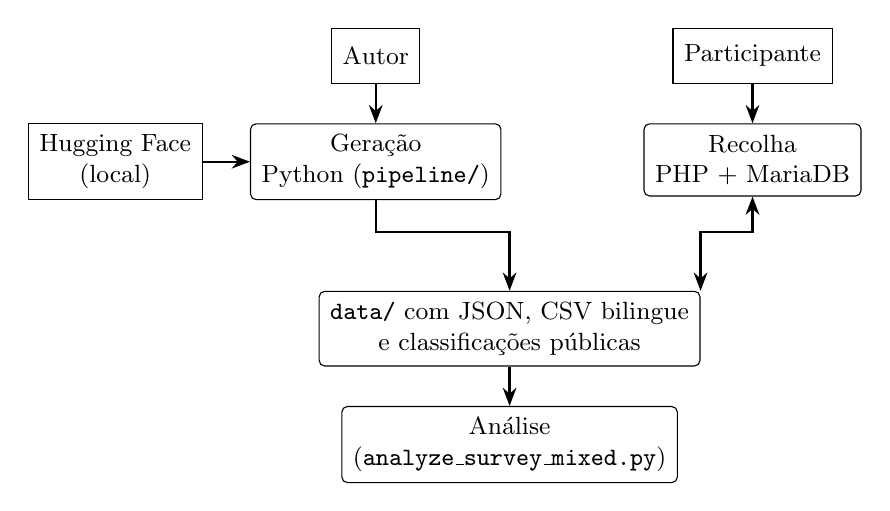
\begin{tikzpicture}[
  node distance=0.5cm and 0.7cm,
  box/.style={draw, rounded corners=2pt, align=center, font=\small, inner sep=4pt, minimum height=0.85cm},
  act/.style={draw, align=center, font=\small, inner sep=4pt, minimum height=0.7cm},
  arr/.style={-{Stealth}, thick}
]
\node[act] (autor) {Autor};
\node[act, right=3.2cm of autor] (part) {Participante};
\node[box, below=of autor] (gen) {Geração\\Python (\texttt{pipeline/})};
\node[box, below=of part] (site) {Recolha\\PHP + MariaDB};
\node[act, left=0.6cm of gen] (hf) {Hugging Face\\(local)};
\node[box, below=1.15cm of gen, xshift=1.7cm] (data) {\texttt{data/} com JSON, CSV bilingue\\e classificações públicas};
\node[box, below=of data] (ana) {Análise\\(\texttt{analyze\_survey\_mixed.py})};
\draw[arr] (autor) -- (gen);
\draw[arr] (hf) -- (gen);
\draw[arr] (part) -- (site);
\draw[arr] (gen.south) -- ++(0,-0.4) -| (data.north);
\draw[{Stealth}-{Stealth}, thick] (site.south) -- ++(0,-0.45) -| (data.north east);
\draw[arr] (data) -- (ana);
\end{tikzpicture}
\caption[Contexto do sistema.]{Contexto do sistema. Geração, recolha e análise comunicam por ficheiros, sem \acrshort{api} em runtime.}
\label{fig:sistema_contexto}
\end{figure}

O analisador emocional, em \texttt{emotion\_analyzer.py}, usa \path{SamLowe/roberta-base-go_emotions} e deriva a \gls{ambivalenciaemocional} com limiar \(\tau = 0{,}10\) \parencite{Demszky2020GoEmotions}. O gerador âncora da época sob avaliação é carregado em \texttt{generator.py} a partir do identificador Hugging Face.

As condições experimentais partilham a mesma intenção de \textit{prompt}.
\begin{itemize}
 \item Na \textit{baseline}, a instrução é de assistente conversacional, sem metadados afectivos.
 \item Na \gls{condicaopipeline}, a mesma instrução inclui o sinal de ambivalência (emoção positiva e negativa dominantes), com a regra de não falar da análise.
\end{itemize}

DialoGPT e BlenderBot usam geradores adaptados às arquitecturas (\textit{causal} e \textit{seq2seq}) \parencite{Zhang2020DialoGPT, Roller2021BlenderBot}. Phi-3-mini e Qwen2.5-3B usam os modelos de conversa no formato de instrução do próprio Hugging Face \parencite{Abdin2024Phi3, Yang2025Qwen25}. O tecto de tokens novos está fixo no protocolo, para respostas curtas (duas a quatro frases nas âncoras instruct), alinhado aos \textit{prompts} da Secção~\ref{sec:impl_prompts}. Os parâmetros de descodificação registados nas 96 células constam da mesma secção.

A pipeline de geração está em módulos com responsabilidades distintas. O \gls{cli}, em \texttt{pipeline.py}, orquestra o lote, com pré-filtro de ambivalência, um gerador por época, células já no disco e \textit{merge}. A orquestração de \textit{uma} célula vive em \texttt{cells.py} (\texttt{run\_cell}). A Figura~\ref{fig:pipeline_componentes} mostra as chamadas. \texttt{prompts.py} não fala com o modelo. \texttt{quality.py} não gera texto. \texttt{generator.py} recebe o \textit{prompt} já formatado. A condição experimental, \textit{baseline} ou \gls{condicaopipeline}, escolhe-se dentro de \texttt{run\_cell}, não no gerador.

\begin{figure}[ht]
\centering
\resizebox{\linewidth}{!}{%
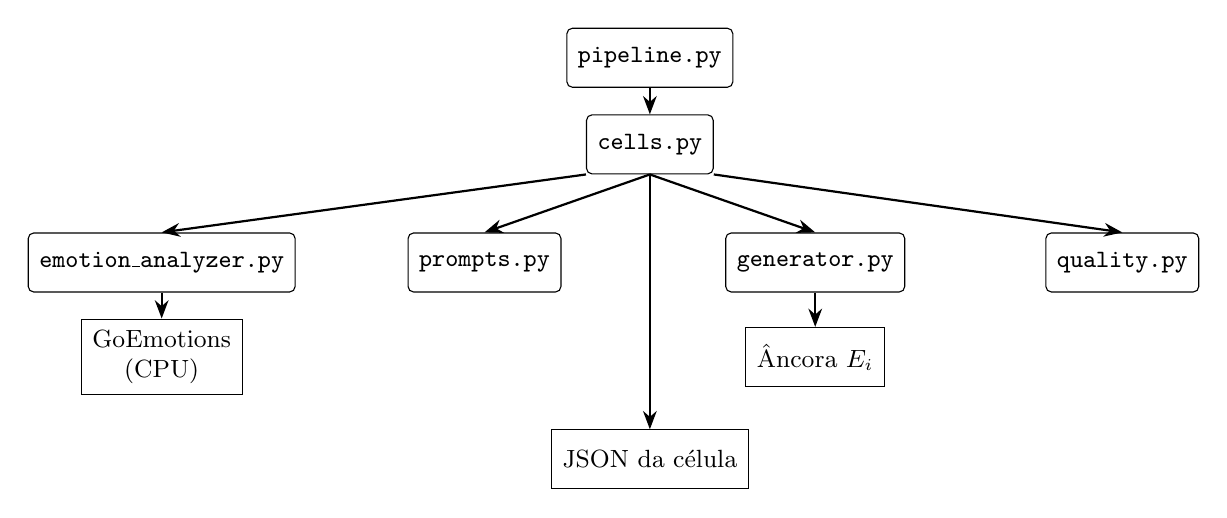
\begin{tikzpicture}[
  box/.style={draw, rounded corners=2pt, align=center, font=\small\ttfamily, inner sep=4pt, minimum height=0.75cm},
  ext/.style={draw, align=center, font=\small, inner sep=4pt, minimum height=0.75cm},
  arr/.style={-{Stealth}, thick}
]
\node[box] (cli) at (0,2.6) {pipeline.py};
\node[box] (cells) at (0,1.5) {cells.py};
\node[box] (ea) at (-6.2,0) {emotion\_analyzer.py};
\node[box] (pr) at (-2.1,0) {prompts.py};
\node[box] (gen) at (2.1,0) {generator.py};
\node[box] (qa) at (6.0,0) {quality.py};
\node[ext] (goe) at (-6.2,-1.2) {GoEmotions\\(CPU)};
\node[ext] (hf) at (2.1,-1.2) {Âncora \(E_i\)};
\node[ext] (json) at (0,-2.5) {JSON da célula};
\draw[arr] (cli) -- (cells);
\draw[arr] (cells.south west) -- (ea.north);
\draw[arr] (cells.south) -- (pr.north);
\draw[arr] (cells.south) -- (gen.north);
\draw[arr] (cells.south east) -- (qa.north);
\draw[arr] (ea) -- (goe);
\draw[arr] (gen) -- (hf);
\draw[arr] (cells.south) -- (json.north);
\end{tikzpicture}%
}
\caption[Componentes da pipeline de geração.]{Componentes da pipeline de geração. O \acrshort{cli} orquestra o lote e grava o JSON. \texttt{run\_cell} produz o registo e chama analisador, \textit{prompts}, gerador e \acrshort{qa}.}
\label{fig:pipeline_componentes}
\end{figure}

\subsection{Fluxo de processamento}
\label{subsec:impl_fluxo}

A Figura~\ref{fig:pipeline_fluxo} resume o que acontece ao texto. O estímulo em inglês entra no GoEmotions \parencite{Demszky2020GoEmotions}, que devolve um vector de scores. A regra \(\tau = 0{,}10\) separa emoções positivas e negativas, escolhe as dominantes de cada valência e marca ambivalência se ambas ultrapassam o limiar. Consoante a condição, constrói-se o \textit{prompt} baseline ou o \textit{prompt} com contexto. O adaptador da âncora \(E_i\) formata essa entrada à arquitectura do modelo. O gerador produz a resposta. A célula é serializada em \gls{json}, exportada para \gls{csv} bilingue, importada para o questionário (MariaDB) e, no fim da recolha, exportada de novo para os scripts de análise do Capítulo~\ref{chap:Chapter5}.

\begin{figure}[ht]
\centering
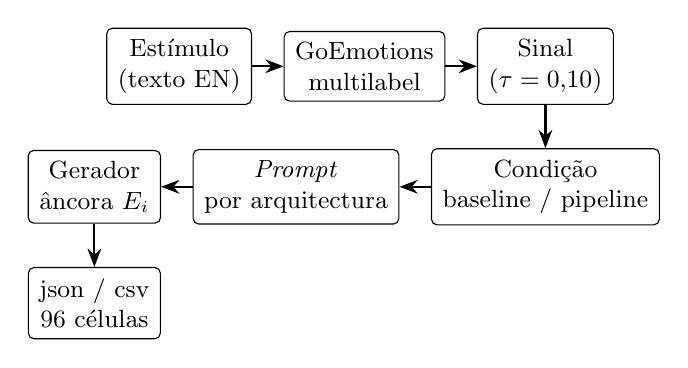
\begin{tikzpicture}[
  node distance=0.55cm and 0.4cm,
  box/.style={draw, rounded corners=2pt, align=center, font=\small, inner sep=4pt, minimum height=0.85cm},
  arr/.style={-{Stealth}, thick}
]
\node[box] (stim) {Estímulo\\(texto EN)};
\node[box, right=of stim] (goe) {GoEmotions\\multilabel};
\node[box, right=of goe] (tau) {Sinal\\(\(\tau=0{,}10\))};
\node[box, below=of tau] (cond) {Condição\\baseline / pipeline};
\node[box, left=of cond] (prompt) {\textit{Prompt}\\por arquitectura};
\node[box, left=of prompt] (gen) {Gerador\\âncora \(E_i\)};
\node[box, below=of gen] (out) {\acrshort{json} / \acrshort{csv}\\96 células};
\draw[arr] (stim) -- (goe);
\draw[arr] (goe) -- (tau);
\draw[arr] (tau) -- (cond);
\draw[arr] (cond) -- (prompt);
\draw[arr] (prompt) -- (gen);
\draw[arr] (gen) -- (out);
\end{tikzpicture}
\caption{Fluxo de dados da pipeline, do estímulo ao JSON da célula, condicionado pelo sinal de ambivalência.}
\label{fig:pipeline_fluxo}
\end{figure}

\subsection{Chamadas de uma célula}
\label{subsec:impl_chamadas}

O lote (\texttt{main} em \texttt{pipeline.py}) percorre os 12 estímulos, as quatro épocas e as duas condições. O Algoritmo~\ref{alg:lote} resume essa orquestração: pré-filtro de ambivalência, um gerador por época, salto das células já gravadas, \texttt{run\_cell} e \texttt{merge\_results}.

\begin{algorithm}[H]
\caption{Geração do lote (\texttt{main} em \texttt{pipeline.py}).}
\label{alg:lote}
\begin{algorithmic}[1]
\Require estímulos, épocas E1--E4, condições \{\textit{baseline}, \textit{pipeline}\}, \(\tau=0{,}10\)
\Ensure células em disco e CSV de itens
\State carregar o analisador GoEmotions
\ForAll{estímulo \(t\)}
  \If{\(t\) não é ambivalente sob \(\tau\)}
    \State descartar \(t\)
  \EndIf
\EndFor
\ForAll{época \(E_i\)}
  \State instanciar \texttt{HFGenerator}(\(E_i\))
  \ForAll{estímulo \(t\) retido \(\times\) condição \(c\)}
    \If{a célula já existe em disco}
      \State saltar
    \Else
      \State \(\textit{row} \gets \mathrm{run\_cell}(t, c)\)
      \State gravar JSON da célula
    \EndIf
  \EndFor
  \State descarregar o gerador
\EndFor
\State \texttt{merge\_results}; exportar CSV de itens
\end{algorithmic}
\end{algorithm}

Uma célula isolada, com o analisador e o gerador já carregados, segue outro caminho. A Figura~\ref{fig:run_cell_seq} mostra as chamadas entre \texttt{cells.py}, o analisador, os \textit{prompts}, o gerador e a \gls{qa}.

\begin{figure}[H]
\centering
\resizebox{\linewidth}{!}{%
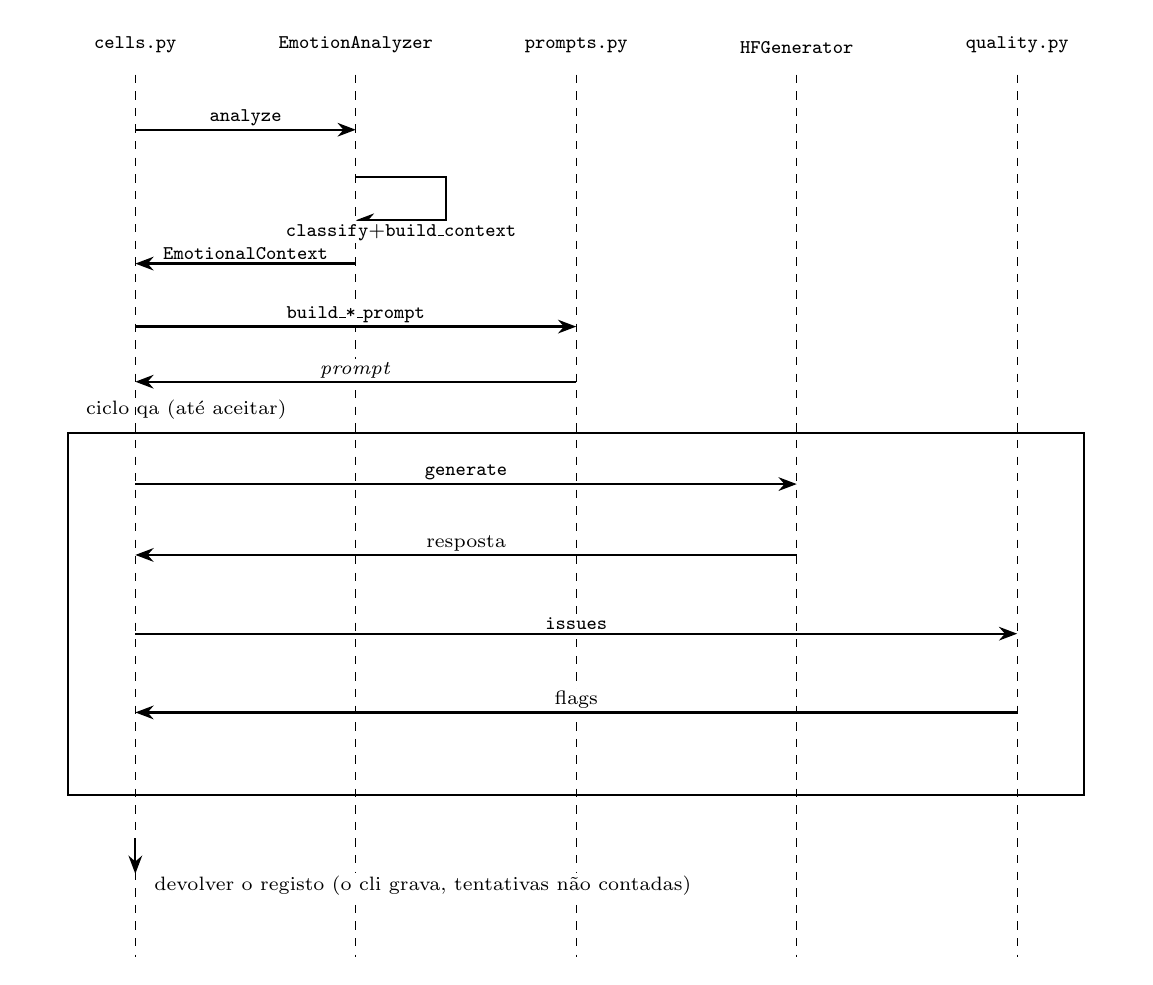
\begin{tikzpicture}[
  font=\scriptsize,
  arr/.style={-{Stealth}, thick},
  lab/.style={font=\scriptsize, inner sep=1pt, fill=white}
]
\foreach \x/\lab in {0/cells.py, 2.8/EmotionAnalyzer, 5.6/prompts.py, 8.4/HFGenerator, 11.2/quality.py} {
  \node[font=\scriptsize\ttfamily, align=center, anchor=south, text width=2.5cm] at (\x, 0.15) {\lab};
  \draw[dashed] (\x, 0) -- (\x, -11.2);
}
% 1. analyze
\draw[arr] (0,-0.7) -- node[lab, above] {\texttt{analyze}} (2.8,-0.7);
% 2. classify on the analyzer lifeline
\draw[arr] (2.8,-1.3) -- ++(1.15,0) -- ++(0,-0.55) -- node[lab, below] {\texttt{classify}+\texttt{build\_context}} ++(-1.15,0);
% 3. context back
\draw[arr] (2.8,-2.4) -- node[lab, above] {\texttt{EmotionalContext}} (0,-2.4);
% 4. prompt
\draw[arr] (0,-3.2) -- node[lab, above] {\texttt{build\_*\_prompt}} (5.6,-3.2);
\draw[arr] (5.6,-3.9) -- node[lab, above] {\textit{prompt}} (0,-3.9);
% QA loop
\draw[thick] (-0.85,-4.55) rectangle (12.05,-9.15);
\node[font=\scriptsize, anchor=south west] at (-0.75,-4.5) {ciclo \acrshort{qa} (até aceitar)};
\draw[arr] (0,-5.2) -- node[lab, above] {\texttt{generate}} (8.4,-5.2);
\draw[arr] (8.4,-6.1) -- node[lab, above] {resposta} (0,-6.1);
\draw[arr] (0,-7.1) -- node[lab, above] {\texttt{issues}} (11.2,-7.1);
\draw[arr] (11.2,-8.1) -- node[lab, above] {flags} (0,-8.1);
% persist
\node[lab, anchor=west] at (0.2,-10.3) {devolver o registo (o \acrshort{cli} grava, tentativas não contadas)};
\draw[arr] (0,-9.7) -- (0,-10.15);
\end{tikzpicture}%
}
\caption[Chamadas de \texttt{run\_cell}.]{Chamadas de \texttt{run\_cell}, com análise, construção do \textit{prompt}, geração e ciclo de \acrshort{qa} até aceitar a resposta.}
\label{fig:run_cell_seq}
\end{figure}

O analisador classifica o enunciado e deriva o contexto (\(\tau = 0{,}10\)). Se a condição é \textit{baseline}, chama-se \texttt{build\_direct\_prompt}. Se é \textit{pipeline}, chama-se \texttt{build\_contextual\_prompt}. O argumento \texttt{arch} vem do gerador (\texttt{causal\_dialogue}, \texttt{seq2seq} ou \texttt{chat}). Os identificadores canónicos do questionário, do tipo \texttt{s01\_\_E1\_\_baseline}, são produzidos por \texttt{sync\_study\_artifacts.py}. O CSV cego opcional de \texttt{export\_blind\_csv} usa \texttt{item\_001}, \texttt{item\_002}, \(\ldots\), e o instrumento não o importa. O Algoritmo~\ref{alg:run_cell} condensa o mesmo ciclo: analisar, construir o \textit{prompt} da condição, gerar e repetir até a \gls{qa} aceitar.

\begin{algorithm}[H]
\caption{Geração de uma célula (\texttt{run\_cell}).}
\label{alg:run_cell}
\begin{algorithmic}[1]
\Require estímulo \(t\), condição \(c\), analisador, gerador âncora
\Ensure registo da célula (JSON)
\State \(\textit{ctx} \gets \mathrm{analyze}(t)\) \Comment{\texttt{EmotionAnalyzer}, \(\tau=0{,}10\)}
\If{\(c = \textit{baseline}\)}
  \State \(\textit{prompt} \gets \mathrm{build\_direct\_prompt}(t, \textit{arch})\)
\Else
  \State \(\textit{prompt} \gets \mathrm{build\_contextual\_prompt}(t, \textit{ctx}, \textit{arch})\)
\EndIf
\State \(\textit{attempt} \gets 0\)
\State \(\textit{issues} \gets \{\texttt{empty}\}\)
\While{\(\textit{issues} \neq \emptyset\)}
  \State \(\mathrm{set\_seed}(42 + \textit{attempt}\times 17 + \textit{cell\_salt})\) \Comment{não constitui amostragem (guloso/beam)}
  \State \(\textit{resp} \gets \mathrm{generate}(\textit{prompt})\)
  \State \(\textit{issues} \gets \mathrm{response\_quality\_issues}(\textit{resp})\)
  \State \(\textit{attempt} \gets \textit{attempt}+1\) \Comment{não é persistido}
\EndWhile
\State \Return célula (\(t\), época, \(c\), \textit{prompt}, \textit{resp}, \textit{ctx}, \(\tau\), semente \(42\))
\end{algorithmic}
\end{algorithm}

O JSON de cada célula (exemplo mínimo, sem o vector \texttt{raw\_emotions}) guarda o contrato entre geração e avaliação:

\begin{verbatim}
{
  "stimulus_id": "s01",
  "epoch_id": "E1",
  "model_id": "microsoft/DialoGPT-medium",
  "condition": "baseline",
  "input": "...",
  "prompt": "...",
  "response": "...",
  "emotion_model": "SamLowe/roberta-base-go_emotions",
  "emotional_context": {
    "ambivalent": true,
    "dominant_positive_emotion": "joy",
    "dominant_negative_emotion": "fear",
    "ambivalence_index": 0.40
  },
  "temperature": null,
  "tau": 0.1,
  "seed": 42,
  "qa_ok": true
}
\end{verbatim}

A \gls{qa} automática (\texttt{quality.py}) aceita a resposta só se a lista de flags estiver vazia. Recusa se o texto está vazio; se é demasiado curto (\(<15\) caracteres em E1, \(<60\) nas outras épocas); se a frase não termina em \texttt{.?!} ou fica cortada a meio (\texttt{and}, \texttt{the}, \ldots); se é um placeholder (\texttt{ok.}, \texttt{i'm sorry.}) ou lixo/repetição; ou se não parece inglês suficiente (sem palavras-função). O ciclo com semente \(42 + \textit{attempt}\times 17 + \textit{cell\_salt}\) existe no código, mas \texttt{attempt} não muda o \textit{prompt}, os feixes nem \texttt{max\_new\_tokens}. Com descodificação gulosa ou \textit{beam search} e temperatura nula, alterar só a semente não constitui amostragem e tende a reproduzir a mesma sequência. Se a célula ficou recusada, a regeneração efectiva foi voltar a executar a mesma célula (mesmo estímulo, época, condição, \textit{prompt} e regra de descodificação) até a \gls{qa} aceitar. O número de recusas não ficou no JSON, que guarda a semente de protocolo \(42\).

%----------------------------------------------------------------------------------------

\section{Implementação da detecção de ambivalência}
\label{sec:impl_deteccao}

A definição e a fórmula de \(A\) estão no Capítulo~\ref{chap:Chapter3}. No código, o mesmo cálculo vive na classe \texttt{EmotionAnalyzer} de \texttt{emotion\_analyzer.py}. O classificador corre em \gls{cpu}. Se não existir pelo menos uma emoção positiva e uma negativa com score \(\ge \tau\), o contexto marca \texttt{ambivalent=false} e o índice \(A\) fica a zero, e na \gls{condicaopipeline}, o \textit{prompt} instruct passa a dizer que não foi detectada ambivalência clara. No lote deste estudo isso não ocorre. Só entram estímulos já confirmados como ambivalentes.

O Algoritmo~\ref{alg:ambivalencia} resume o passo de detecção. O limiar \(\tau = 0{,}10\) é o mesmo da metodologia, mais permissivo do que um corte em \(0{,}5\), escolhido para activar o sinal nos textos redigidos com contraste explícito, sem pretender ser um limiar óptimo de classificação.

\begin{algorithm}[ht]
\caption{Derivação do sinal de ambivalência a partir do \mbox{GoEmotions}.}
\label{alg:ambivalencia}
\begin{algorithmic}[1]
\Require texto \(t\), limiar \(\tau = 0{,}10\), conjuntos \(E^+\) e \(E^-\)
\Ensure contexto emocional (ambivalente, \(e_p^\ast\), \(e_n^\ast\), \(A\))
\State \(S \gets \mathrm{classify}(t)\) \Comment{scores \(s_i \in [0,1]\) por rótulo GoEmotions}
\State \(e_p^\ast, s_p^\ast \gets \arg\max_{e \in E^+} S(e)\)
\State \(e_n^\ast, s_n^\ast \gets \arg\max_{e \in E^-} S(e)\)
\If{\(s_p^\ast \ge \tau\) \textbf{and} \(s_n^\ast \ge \tau\)}
  \State \(\mathrm{ambivalent} \gets \mathbf{true}\)
  \State \(A \gets \min(s_p^\ast, s_n^\ast)\)
\Else
  \State \(\mathrm{ambivalent} \gets \mathbf{false}\); \(A \gets 0\)
\EndIf
\State \Return \((\mathrm{ambivalent}, e_p^\ast, e_n^\ast, A)\)
\end{algorithmic}
\end{algorithm}

%----------------------------------------------------------------------------------------

\section{Geradores âncora}
\label{sec:impl_modelos}

Os quatro geradores são as instâncias públicas dos marcos da Secção~\ref{sec:marcos_historicos}, as mesmas da tabela do Capítulo~\ref{chap:Chapter3}. DialoGPT-medium é a âncora de diálogo \textit{open-domain} frequente na literatura \parencite{Zhang2020DialoGPT}. BlenderBot representa a linha de diálogo social \parencite{Roller2021BlenderBot}. Phi-3-mini-Instruct é o \gls{llm} \textit{instruction-tuned} de código aberto dessa geração \parencite{Abdin2024Phi3}. Qwen2.5-Instruct é o \gls{llm} alinhado recente \parencite{Yang2025Qwen25}.

Identificadores Hugging Face:
\begin{itemize}
 \item E1: \texttt{microsoft/DialoGPT-medium};
 \item E2: \path{facebook/blenderbot-400M-distill};
 \item E3: \texttt{microsoft/Phi-3-mini-4k-instruct};
 \item E4: \texttt{Qwen/Qwen2.5-3B-Instruct}.
\end{itemize}

A geração corre localmente, em Python, com Hugging Face Transformers, sem \glspl{api} proprietárias \parencite{Wolf2020Transformers}. As dependências principais são \texttt{transformers} e \texttt{torch}, no \texttt{requirements.txt} do repositório. Quem replicar usa estes IDs. Nas 96 células avaliadas, a semente é 42 e \(\tau = 0{,}10\).

\subsection{Geração e adaptação por modelo}
\label{subsec:impl_manipulacao}

Não existe um \textit{prompt} universal. A manipulação conceptual é a mesma, o par de emoções dominantes, mas a realização técnica não. DialoGPT espera o enunciado em formato de diálogo causal \parencite{Zhang2020DialoGPT}; o BlenderBot é \textit{seq2seq} e trata a entrada como uma única sequência \parencite{Roller2021BlenderBot}; Phi-3 e Qwen usam o formato de conversa por instrução \parencite{Abdin2024Phi3, Yang2025Qwen25}. Injectar o mesmo bloco de metadados nas quatro âncoras seria, em E1 e E2, um input que esses modelos nunca viram no treino. A Tabela~\ref{tab:manipulacao_prompt} resume a forma adoptada.

\begin{table}[ht]
\centering
\caption{Formato do sinal de ambivalência por gerador âncora.}
\label{tab:manipulacao_prompt}
\begin{tabular}{ll>{\raggedright\arraybackslash}p{6.4cm}}
\hline
Época & Arquitectura & Forma da manipulação \\
\hline
E1 & Diálogo causal & Frase curta entre utilizador e assistente: ``(The user seems ambivalent: joy and fear.)'' \\
E2 & Seq2seq & Anotação sufixada ao enunciado: ``[emotional ambivalence: joy and fear]'' \\
E3/E4 & Chat instruct & Bloco de metadados + instruções para não mencionar a análise \\
\hline
\end{tabular}
\end{table}

O sinal entra no contexto de geração de forma adaptada a cada arquitectura (Tabela~\ref{tab:manipulacao_prompt}): o mesmo par de emoções dominantes, realizado como o modelo espera o input.

%----------------------------------------------------------------------------------------

\section{Prompts: um estímulo, quatro geradores âncora}
\label{sec:impl_prompts}

Os exemplos abaixo usam o estímulo s01 (promoção com medo de impostor), o mesmo texto nas oito células. Assim o leitor vê o efeito da arquitectura sobre a mesma entrada, em vez de uma colecção de excertos soltos. As respostas geradas correspondentes estão no Apêndice~\ref{AppendixB}.

\paragraph{E1 (DialoGPT), baseline.}
\begin{verbatim}
User: I am so proud and happy about this promotion, but I am
also scared and anxious that everyone will soon see that I
do not deserve it.
Assistant:
\end{verbatim}

\paragraph{E1 (DialoGPT), pipeline.}
\begin{verbatim}
User: I am so proud and happy about this promotion, but I am
also scared and anxious that everyone will soon see that I
do not deserve it.
(The user seems ambivalent: joy and fear.)
Assistant:
\end{verbatim}

\paragraph{E2 (BlenderBot), baseline.}
A entrada \textit{seq2seq} é o enunciado do utilizador, sem prefixo de papéis:
\begin{verbatim}
I am so proud and happy about this promotion, but I am also
scared and anxious that everyone will soon see that I do not
deserve it.
\end{verbatim}

\paragraph{E2 (BlenderBot), pipeline.}
O sinal é sufixado ao mesmo enunciado:
\begin{verbatim}
I am so proud and happy about this promotion, but I am also
scared and anxious that everyone will soon see that I do not
deserve it. [emotional ambivalence: joy and fear]
\end{verbatim}

\paragraph{E3/E4 (instruct), baseline.}
\begin{verbatim}
You are a conversational assistant.

User message:
I am so proud and happy about this promotion, but I am also
scared and anxious that everyone will soon see that I do not
deserve it.

Produce a clear, helpful, and natural answer in English.
Write 2 to 4 complete sentences and stop.
\end{verbatim}

\paragraph{E3/E4 (instruct), pipeline.}
\begin{verbatim}
You are a conversational assistant.

User message:
I am so proud and happy about this promotion, but I am also
scared and anxious that everyone will soon see that I do not
deserve it.

Additional emotional context:
The user's message appears to contain emotional ambivalence.
The dominant positive emotion is joy.
The dominant negative emotion is fear.

Use this emotional context only as background information
when answering.
Do not mention the emotional analysis, emotion labels, scores,
or pipeline.
Do not change your normal response style solely because this
metadata is present.

Produce a clear, helpful, and natural answer in English.
Write 2 to 4 complete sentences and stop.
\end{verbatim}

\subsection{Proveniência e parâmetros de geração}
\label{subsec:impl_proveniencia}

Os parâmetros efectivos das 96 células estão no \gls{json} arquivado (\texttt{appendices/data/\allowbreak all\_results.json}), com \(\tau = 0{,}10\) e semente 42. A temperatura registada é nula em todas as 96 células (Tabela~\ref{tab:gen_params}). O tecto \texttt{max\_new\_tokens} é 128 em E1 e E2 e 160 em E3 e E4; no DialoGPT, com \textit{beam search}, o tecto efectivo é \(\min(80, \texttt{max\_new\_tokens})\).

\begin{table}[ht]
\centering
\caption[Parâmetros de geração por época.]{Parâmetros de geração registados em \texttt{all\_results.json} por época (96 células).}
\label{tab:gen_params}
\begin{tabular}{lcp{6.8cm}}
\hline
Época & Células & Descodificação \\
\hline
E1 DialoGPT & 24 & \(T=\texttt{null}\); \textit{beam search} (\texttt{num\_beams=5}) \\
E2 BlenderBot & 24 & \(T=\texttt{null}\); gulosa \\
E3 Phi-3 & 24 & \(T=\texttt{null}\); gulosa \\
E4 Qwen2.5 & 24 & \(T=\texttt{null}\); gulosa \\
\hline
\end{tabular}
\end{table}

\texttt{HFGenerator.generate} recebe o \textit{prompt} já formatado e tokeniza-o. Nas âncoras instruct E3 e E4 aplica \texttt{apply\_chat\_template} com \texttt{add\_generation\_prompt}. No DialoGPT a descodificação é \textit{beam search} com cinco feixes. Nas âncoras E2--E4 é gulosa (\texttt{do\_sample=False}, um feixe). No DialoGPT corta-se o texto a partir de um falso turno seguinte do utilizador, padrão frequente neste modelo. A condição experimental, \textit{baseline} ou \gls{condicaopipeline}, não é a única diferença técnica entre âncoras. Também mudam a arquitectura, o formato do \textit{prompt} e a estratégia de descodificação.

%----------------------------------------------------------------------------------------

\section{Estímulos e geração em lote}
\label{sec:impl_batch}

Foram redigidos e revistos pelo autor 12 estímulos em inglês para expressar ambivalência explícita e plausível, com sinais de valências opostas no mesmo enunciado. Antes da geração, o GoEmotions confirma a ambivalência \parencite{Demszky2020GoEmotions}, e só entram no lote os textos em que essa condição se verifica (com o limiar \(\tau\) do Capítulo~\ref{chap:Chapter3}). A tabela dos estímulos e das valências dominantes consta da Secção~\ref{sec:materiais}.

O lote percorre, para cada estímulo, as quatro épocas e as duas condições: \(12 \times 4 \times 2 = 96\) células. Cada célula fica guardada em \gls{json} (estímulo, modelo, condição, \textit{prompt}, resposta, contexto emocional e parâmetros). Também se exporta um \gls{csv} bilingue (EN/PT) com identificadores estáveis do tipo \texttt{sXX\_\_EY\_\_condition} (por exemplo \texttt{s01\_\_E1\_\_baseline}) para o questionário cego. Época, gerador âncora e condição ficam na base de dados para a análise, mas o avaliador não as vê.

As 96 respostas dos geradores âncora tiveram uma revisão mínima, pelas mesmas regras da \gls{qa} automática. Células recusadas (vazias, em inglês inválido, ininteligíveis ou malformadas) voltaram a ser executadas na mesma célula (o mesmo estímulo, época, condição, \textit{prompt} e descodificação), até a \gls{qa} aceitar. Não se escolheu a «melhor» entre várias válidas, nem se editou o texto. O número de células regeneradas não ficou registado no log; o lote avaliado são as 96 células finais. Não há células em falta. Fora desses casos, o conteúdo não foi revisto nem editado. Editar o texto gerado teria contaminado a comparação entre geradores âncora e condições. Os textos completos estão no Apêndice~\ref{AppendixB}.

%----------------------------------------------------------------------------------------

\section{Instrumento de avaliação}
\label{sec:impl_questionario}

A avaliação humana corre num questionário online em \gls{php} e MariaDB, alojado num servidor do estudo para a recolha. As 96 células entram a partir do \gls{csv} da pipeline. Um script no repositório (\texttt{sync\_study\_artifacts.py}) mantém alinhados o texto da dissertação, o \gls{csv} de estímulos e o catálogo do instrumento. Os artefactos canónicos da geração estão em \texttt{appendices/data/}: \texttt{questionnaire\_items.csv} (96 itens) e \texttt{all\_results.json}.

O participante escolhe idioma (português ou inglês), dá consentimento (\(\ge 18\) anos), faz um item de prática (não conta), responde cerca de 24 itens cegos em Likert 1--7, pode continuar com mais itens ou parar, faz a verificação de atenção e chega ao agradecimento. Cada resposta é gravada de imediato. Não se pedem dados demográficos. Se a pessoa voltar no mesmo browser, a sessão retoma-se sem criar outro participante. A ordem do bloco mínimo e dos extras vem de um plano de rotação ligado ao identificador da sessão. O script \texttt{assign.php} escolhe o par de blocos (\(\mathrm{id}\bmod 15\)) e baralha a ordem com semente \(42 + \textit{participantId}\). Essa atribuição não é um ecrã. Corre quando o consentimento é aceite.

A Figura~\ref{fig:instrumento_estados} mostra os estados da sessão, alinhados a \texttt{last\_step} e às páginas PHP. A linha a tracejado é a retoma pelo cookie \texttt{prepd\_resume}, via \texttt{resume\_destination()}. Sessão concluída vai para o agradecimento. Recusa ou abandono vai para \texttt{declined}. Sem consentimento, o fluxo volta ao consentimento. Prática ou itens em falta voltam ao questionário. Bloco mínimo feito sem extras desbloqueados vai para a oferta de continuar.

\begin{figure}[ht]
\centering
\resizebox{\linewidth}{!}{%
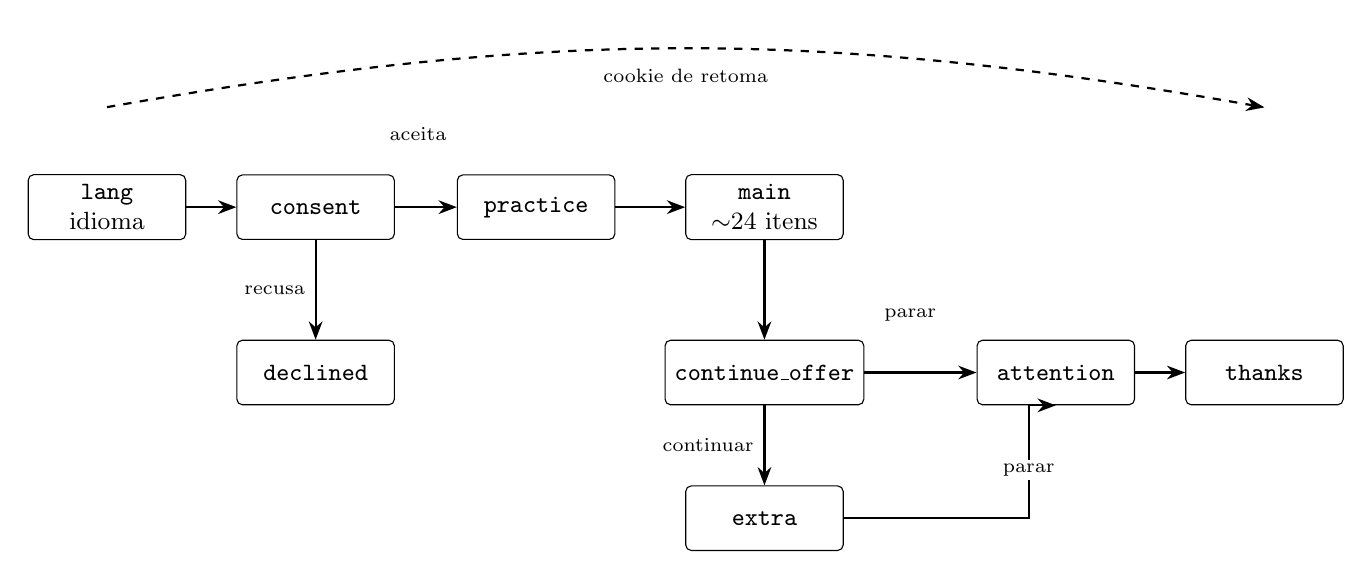
\begin{tikzpicture}[
  st/.style={draw, rounded corners=2pt, align=center, font=\small, inner sep=3.5pt, minimum height=0.82cm, minimum width=2.0cm},
  arr/.style={-{Stealth}, thick},
  lab/.style={font=\scriptsize, fill=white, inner sep=1.5pt}
]
\node[st] (lang) at (0,2.55) {\texttt{lang}\\idioma};
\node[st] (cons) at (2.65,2.55) {\texttt{consent}};
\node[st] (prac) at (5.45,2.55) {\texttt{practice}};
\node[st] (main) at (8.35,2.55) {\texttt{main}\\\(\sim\)24 itens};
\node[st] (dec) at (2.65,0.45) {\texttt{declined}};
\node[st] (off) at (8.35,0.45) {\texttt{continue\_offer}};
\node[st] (att) at (12.05,0.45) {\texttt{attention}};
\node[st] (th) at (14.7,0.45) {\texttt{thanks}};
\node[st] (extra) at (8.35,-1.4) {\texttt{extra}};
\node[lab] at (3.95,3.48) {aceita};
\node[lab] at (7.35,4.22) {cookie de retoma};
\node[lab] at (10.2,1.18) {parar};
\draw[arr] (lang) -- (cons);
\draw[arr] (cons) -- (prac);
\draw[arr] (cons) -- node[lab, left=2pt] {recusa} (dec);
\draw[arr] (prac) -- (main);
\draw[arr] (main) -- (off);
\draw[arr] (off) -- node[lab, left=2pt] {continuar} (extra);
\draw[arr] (off) -- (att);
\draw[arr] (extra.east) -- ++(2.35,0) |- node[lab, pos=0.14, above=2pt] {parar} (att.south);
\draw[arr] (att) -- (th);
\draw[arr, dashed] ([yshift=0.85cm]lang.north) to[out=10, in=170] ([yshift=2.95cm]th.north);
\end{tikzpicture}%
}
\caption[Máquina de estados do instrumento.]{Máquina de estados do instrumento, com os ecrãs PHP e a retoma da sessão a tracejado.}
\label{fig:instrumento_estados}
\end{figure}

A Figura~\ref{fig:ui_participante} mostra o ecrã que o avaliador vê. O enunciado do utilizador, a resposta do assistente e a escala de sete pontos aparecem sem indicação de modelo ou condição.

\begin{figure}[ht]
\centering
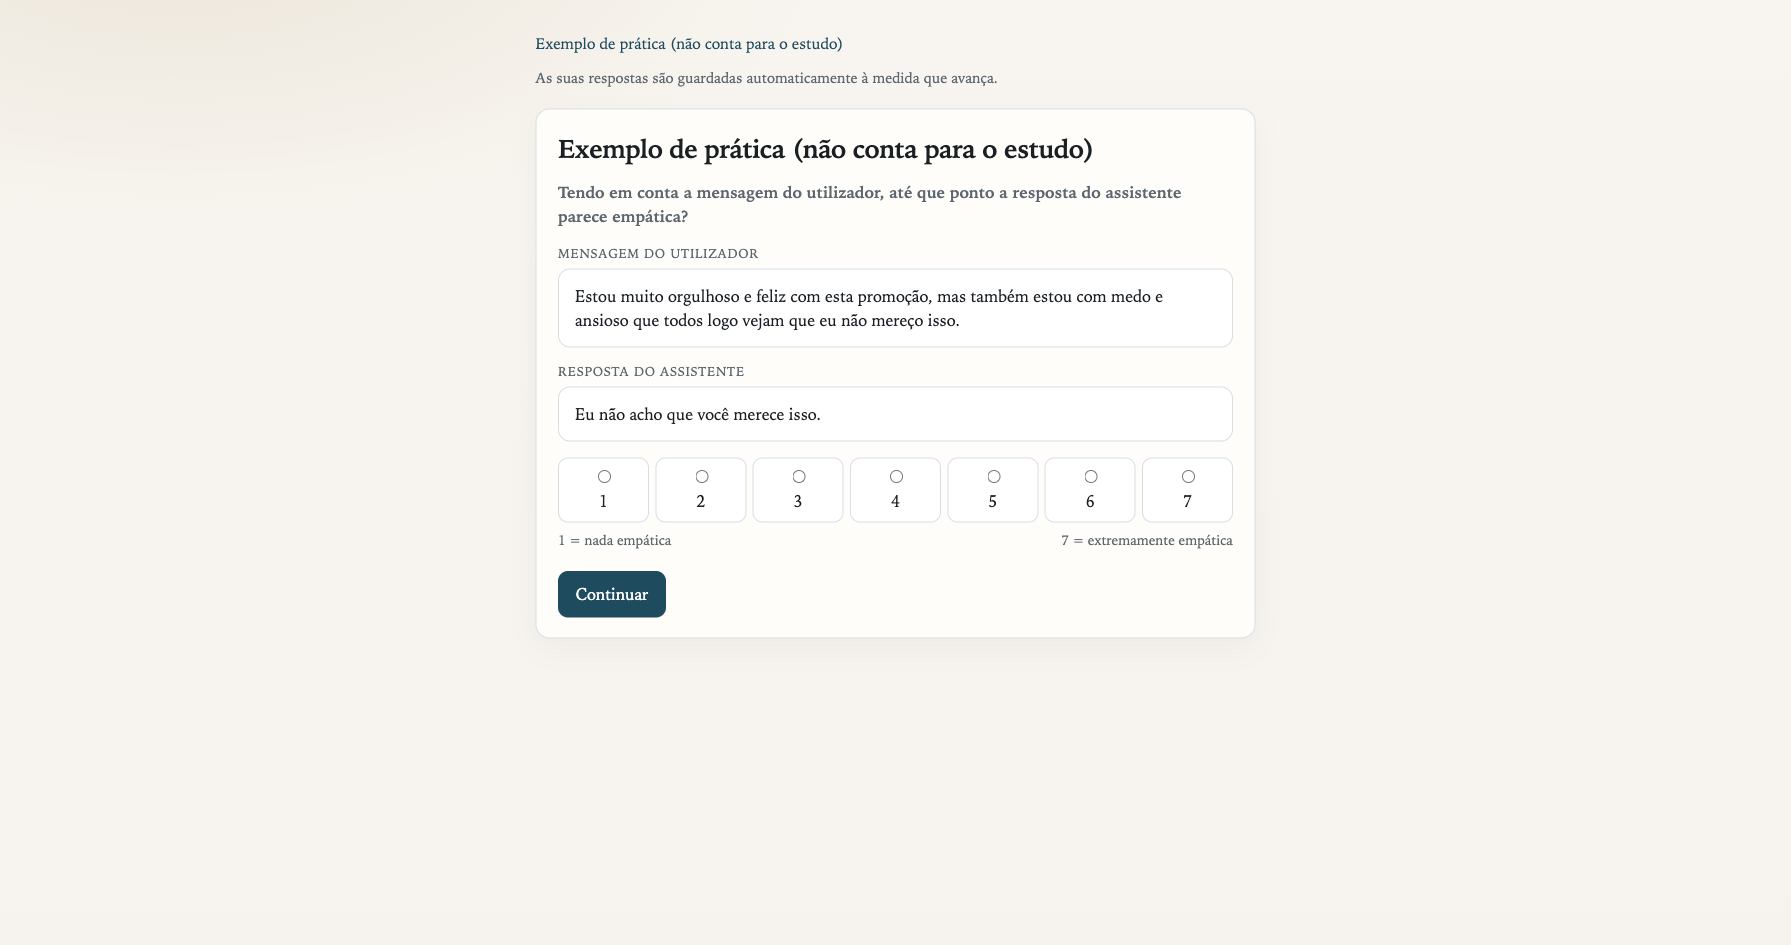
\includegraphics[width=0.92\textwidth]{ch4/assets/survey-participante.png}
\caption[Interface do participante.]{Interface do participante: item de prática, enunciado, resposta e escala Likert 1--7. O avaliador não vê o modelo nem a condição.}
\label{fig:ui_participante}
\end{figure}

A Figura~\ref{fig:ui_admin} mostra o painel de administração, protegido por palavra-passe. Inclui totais de itens, participantes e classificações, e a exportação \gls{csv}.

\begin{figure}[ht]
\centering
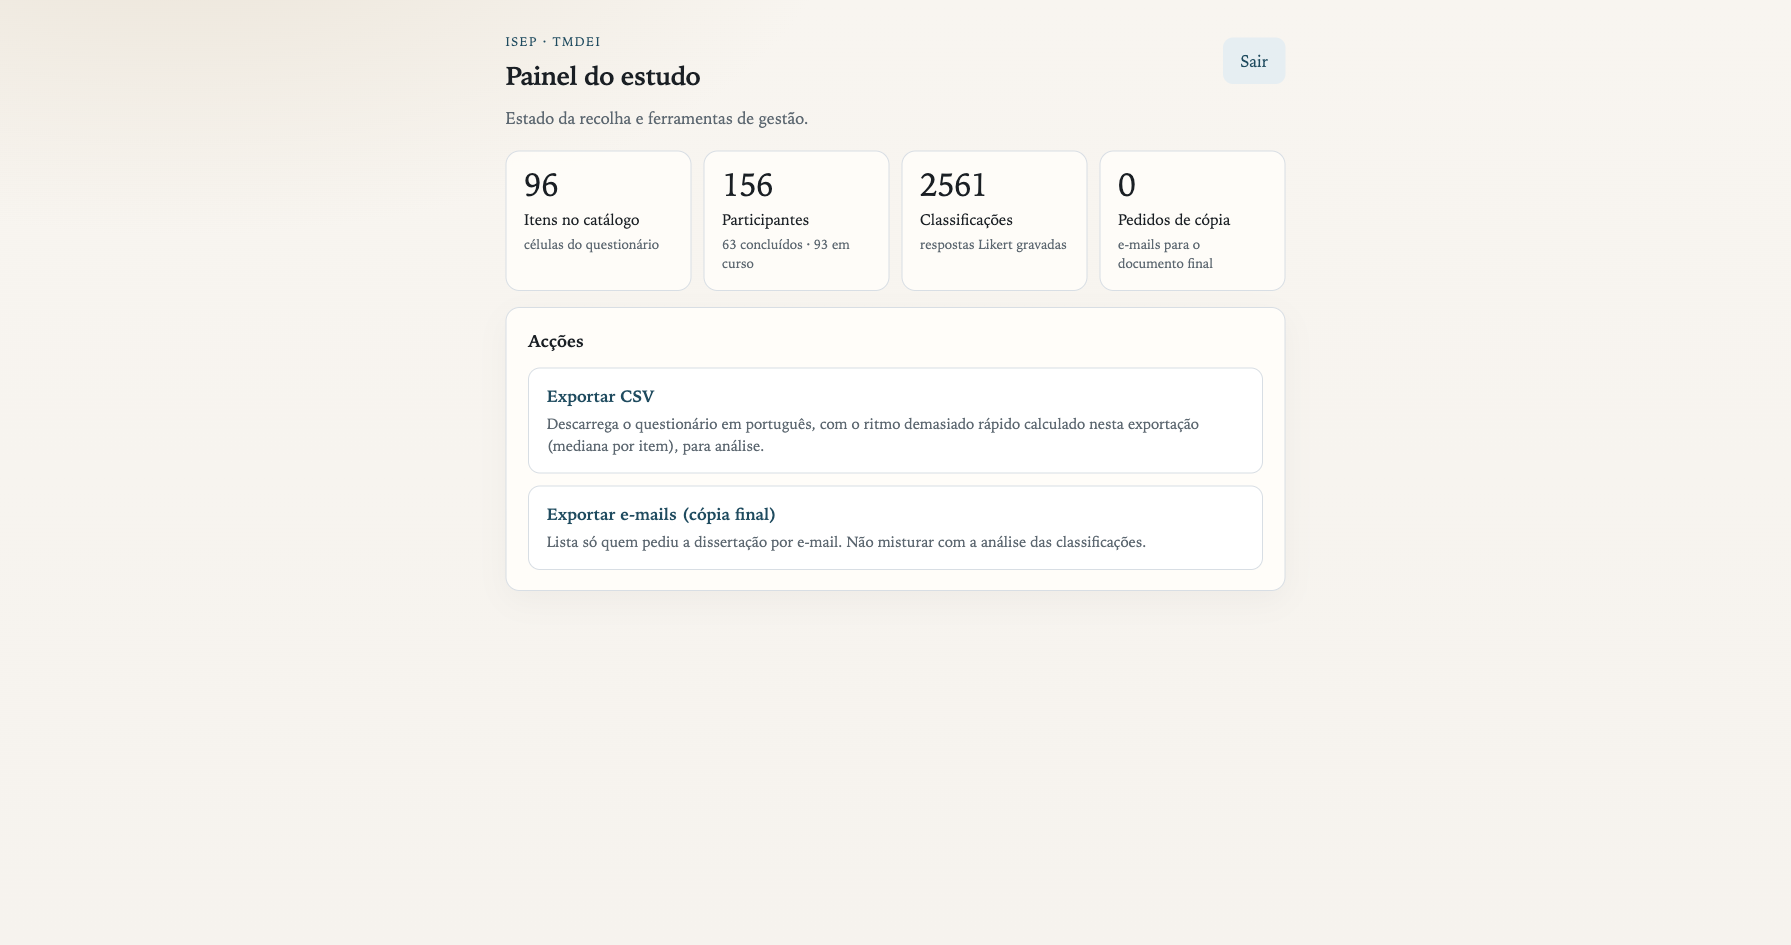
\includegraphics[width=0.92\textwidth]{ch4/assets/admin-painel.png}
\caption[Painel de administração do instrumento.]{Painel de administração do instrumento, com os totais da recolha canónica: 96 itens, 156 participantes, 2561 classificações no ficheiro bruto.}
\label{fig:ui_admin}
\end{figure}

Consentimento e instruções Likert estão na interface; o Apêndice~\ref{AppendixA} resume o material apresentado aos participantes.

\subsection{Tradução e interface bilingue}
\label{subsec:impl_traducao}

{\emergencystretch=2em
Os estímulos e as respostas foram gerados em inglês, e a interface do questionário apresenta versões em português e em inglês. O catálogo bilingue (\path{appendices/data/questionnaire_items_i18n.csv}) foi produzido pelo script \texttt{sync\_study\_artifacts.py}: tradução automática EN\(\rightarrow\)PT via \texttt{deep\_translator.GoogleTranslator}, com cache em \path{appendices/data/translation_cache.json}. A tradução para português foi revista por humano, para garantir que estava correcta. A exportação administrativa localiza cabeçalhos e valores categóricos (por exemplo, \textit{Português}/\textit{Inglês}, \textit{linha de base}/\textit{pipeline}, \textit{concluído}). No filtro estrito, 46 participantes usaram português (1770 classificações) e 6 inglês (246). A língua da sessão fica como limitação e covariável futura, e não entra como factor formal nesta análise.
\par}

\subsection{Critério de ritmo demasiado rápido}
\label{subsec:impl_ritmo}

A exportação calcula um indicador de ritmo relativo, em vez de um limiar fixo de duração da sessão. O procedimento, implementado em \texttt{export\_survey.php}, usa o \gls{dam} da distribuição de ritmos e é o seguinte:

\begin{enumerate}
 \item tempo por resposta = diferença entre os valores de \texttt{respondido em} de itens consecutivos do mesmo participante (ordenado por posição); ignora-se o primeiro item e intervalos superiores a 600\,s (pausas);
 \item mediana por \texttt{código do item} nesta exportação;
 \item ritmo relativo de cada resposta = tempo / mediana do item; o ritmo típico do participante é a mediana dessas razões;
 \item entre concluídos com atenção correcta e pelo menos dez tempos válidos, limiar inferior \(\textit{mediana} - 2{,}5 \times \text{\acrshort{dam}}\);
 \item participante abaixo do limiar, motivo de exclusão ``ritmo demasiado rápido''.
\end{enumerate}

O \gls{csv} inclui as colunas de tempo por resposta, mediana do item, ritmo relativo e indicador de ritmo demasiado rápido. Nesta amostra, o critério marcou quatro participantes, e o filtro estrito da análise principal exclui-os.

\subsection{Item de prática}
\label{subsec:impl_pratica}

Com \texttt{practice\_item\_id} nulo na configuração, o item de prática é o primeiro do catálogo importado: \texttt{s01\_\_E1\_\_baseline} (DialoGPT, baseline, estímulo s01). Esse contacto inicial não conta para o mínimo da sessão, mas a mesma célula pode voltar a aparecer na rotação pontuada (na análise estrita, 25 participantes reavaliaram-na uma vez). Uma resposta de baixa empatia no DialoGPT pode, assim, ancorar a leitura da escala Likert. O Capítulo~\ref{chap:Chapter5} reporta uma sensibilidade que exclui essas classificações, e em trabalho futuro recomenda-se um item neutro dedicado que nunca reentre na amostra.

%----------------------------------------------------------------------------------------

\section{Modelo de dados}
\label{sec:impl_dados}

O instrumento persiste três tabelas em MariaDB, definidas no esquema \gls{sql} (\texttt{site/sql/schema.sql}). A Figura~\ref{fig:erd} mostra os campos que importam para a análise. A \gls{pk} de cada tabela e as \glspl{fk} em \texttt{ratings} ligam sessão e célula. A tabela \texttt{items} guarda as 96 células (identificador opaco, estímulo, textos EN/PT, época, modelo, condição). A tabela \texttt{participants} guarda a sessão: língua, consentimento, estado (\textit{in\_progress} / \textit{completed}), token de retoma, verificação de atenção, motivo de exclusão e marcas temporais. A tabela \texttt{ratings} liga participante a item, com a nota Likert, a posição na sequência e o instante da resposta.

\begin{figure}[ht]
\centering
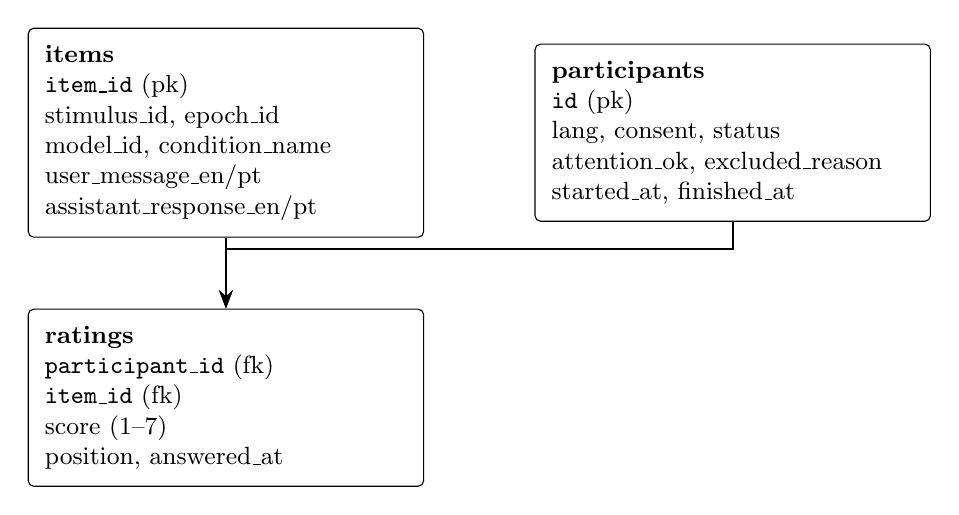
\begin{tikzpicture}[
  entity/.style={draw, rounded corners=2pt, align=left, font=\small, inner sep=6pt, text width=4.6cm},
  arr/.style={-{Stealth}, thick}
]
\node[entity] (items) {\textbf{items}\\\texttt{item\_id} (\acrshort{pk})\\stimulus\_id, epoch\_id\\model\_id, condition\_name\\user\_message\_en/pt\\assistant\_response\_en/pt};
\node[entity, right=1.4cm of items] (part) {\textbf{participants}\\\texttt{id} (\acrshort{pk})\\lang, consent, status\\attention\_ok, excluded\_reason\\started\_at, finished\_at};
\node[entity, below=0.9cm of items] (rat) {\textbf{ratings}\\\texttt{participant\_id} (\acrshort{fk})\\ \texttt{item\_id} (\acrshort{fk})\\score (1--7)\\position, answered\_at};
\draw[arr] (part.south) -- ++(0,-0.35) -| (rat.north);
\draw[arr] (items.south) -- (rat.north);
\end{tikzpicture}
\caption{Modelo de dados do instrumento: células, sessões e classificações.}
\label{fig:erd}
\end{figure}

%----------------------------------------------------------------------------------------

\section{Fluxo de exportação e análise}
\label{sec:impl_export}

A cadeia de replicabilidade fecha o contrato da Figura~\ref{fig:sistema_contexto}. A pipeline grava \path{all_results.json} e o CSV de itens. O script \texttt{sync\_study\_artifacts.py} produz o catálogo bilingue com identificadores estáveis \texttt{sXX\_\_EY\_\_condition}. O painel de administração importa esse CSV para MariaDB. Durante a recolha, cada Likert fica em \texttt{ratings}. No fim, \texttt{export\_survey.php} gera o CSV em português, já com as colunas de ritmo relativo. Os scripts de análise (\texttt{analyze\_survey\_export.py}, \texttt{analyze\_survey\_mixed.py}) lêem esse ficheiro, aplicam os filtros (estrito, atenção, todos) e estimam médias, \(\Delta\) descritivos e o modelo misto cruzado. O output do misto, filtro estrito, está em \path{appendices/data/mixed_crossed_strict.json} e alimenta as tabelas do Capítulo~\ref{chap:Chapter5}.

%----------------------------------------------------------------------------------------

% Chapter 5
% Resultados

\chapter{Resultados e Discussão}
\label{chap:Chapter5}

Este capítulo apresenta os resultados da avaliação humana cega e a sua discussão à luz da hipótese formulada no Capítulo~\ref{chap:Chapter1}, segundo a qual o diferencial de empatia associado ao sinal explícito de ambivalência depende do gerador âncora seleccionado.

A análise usa o export administrativo do questionário, processado no repositório experimental (\url{https://github.com/marcelobarrosow/isep-mestrado-dissertacao}) pelos scripts \texttt{analyze\_survey\_export.py} e \texttt{analyze\_survey\_mixed.py}. O ficheiro está em português (cabeçalhos e valores categóricos) e inclui colunas de ritmo de resposta calculadas na exportação.

%----------------------------------------------------------------------------------------

\section{Procedimento de análise}
\label{sec:res_procedimento}

Para cada classificação Likert (1--7) com identificador de célula válido, agregaram-se as pontuações por época \(E1\)--\(E4\) e condição (\textit{baseline} vs condição com sinal), estimando
\[
\Delta_e = \overline{\text{empatia}}_{\text{pipeline},e} - \overline{\text{empatia}}_{\text{baseline},e}.
\]

A análise principal adopta o filtro \textit{estrito}: participantes com estado concluído, verificação de atenção correcta (valor 2 na escala de controlo no final da sessão) e sem motivo de exclusão por ritmo demasiado rápido. Este último critério é calculado na exportação, não na base de dados. Para cada item, estima-se o tempo entre respostas consecutivas (ignorando o primeiro item e pausas superiores a 600\,s); calcula-se a mediana por item na própria amostra; o ritmo relativo de cada participante é a mediana das razões tempo/mediana do item; entre concluídos com atenção correcta e pelo menos dez tempos válidos, define-se o limiar robusto \(\textit{mediana} - 2{,}5 \times \text{\gls{dam}}\). Participantes abaixo desse limiar são marcados como ritmo demasiado rápido e excluídos da análise principal. Nesta amostra, apenas quatro participantes foram excluídos por esse motivo.

A inferência principal ajusta a dependência dos dados com um modelo linear misto de efeitos aleatórios \textit{cruzados} (participante \(\times\) item), estimado por \gls{reml} (\texttt{statsmodels}), com efeitos fixos \(\textit{condição} \times \textit{época}\) \parencite{Baayen2008Mixed}. Os contrastes reportados são os efeitos marginais da \gls{condicaopipeline} face à \gls{baseline} em cada época, com \gls{se} e intervalos de confiança a 95\%. A interacção global é testada por um contraste de Wald sobre os três termos \(\textit{condição}\times\textit{época}\).

Como descrição suplementar, reportam-se médias por célula, tamanhos de efeito \(d\) de Cohen e testes \(t\) de Welch ao nível da classificação. Estes testes ignoram o aninhamento e o cruzamento entre participante e item, e não constituem a inferência principal. Como sensibilidades, repetiu-se o cálculo descritivo de \(\Delta_e\) (i) com todos os participantes de atenção correcta (\textit{atenção}), (ii) com todas as classificações do export (\textit{todos}), (iii) com peso igual por participante, e (iv) excluindo o item de prática quando este reapareceu na rotação.

%----------------------------------------------------------------------------------------

\section{Cobertura da amostra}
\label{sec:res_amostra}

A Tabela~\ref{tab:amostra_recolha} resume a cobertura, a mesma do funil da Secção~\ref{sec:recrutamento}. A análise principal assenta nas 2016 classificações dos 52 participantes no filtro estrito.

\begin{table}[ht]
\centering
\caption{Cobertura da recolha humana.}
\label{tab:amostra_recolha}
\begin{tabular}{lc}
\hline
Indicador & Valor \\
\hline
Participantes iniciados & 156 \\
Participantes concluídos & 63 \\
Atenção correcta & 56 \\
Ritmo demasiado rápido & 4 \\
Análise principal (filtro estrito) & 52 \\
Classificações Likert na análise principal & 2016 \\
\hline
\end{tabular}
\end{table}

Destes, 46 usaram português (1770 classificações) e 6 inglês (246 classificações). Os números abaixo referem-se a este recorte, salvo indicação em contrário.

O recrutamento foi de conveniência, por bola de neve na rede pessoal e académica. Quem completa o estudo pode diferir de quem abandona: mais paciência, mais interesse no tema, outra tolerância a respostas fracas, em particular as de E1. Sem demografia, essa diferença não se testa. As classificações de quem ficou são as que o desenho permite analisar, e a generalização para utilizadores quaisquer de chatbot fica limitada.

O volume de respostas por participante é desigual: a mediana é 24 itens; 35 participantes avaliaram exactamente 24 células; 7 avaliaram as 96 células possíveis (672 classificações, cerca de um terço do total). Esta auto-selecção de extras é uma limitação, mas a sensibilidade com peso igual por participante mitiga, em parte, a influência dos avaliadores com maior volume.

%----------------------------------------------------------------------------------------

\section{Resultados descritivos por época}
\label{sec:res_por_epoca}

O padrão mais nítido não é o diferencial entre condições, e sim o nível absoluto de empatia: as médias sobem de cerca de \(1{,}5\) em E1 para cerca de \(6{,}1\) em E3 (e \(5{,}4\) em E4), nas duas condições. O detalhe por âncora segue.

\subsection{E1: DialoGPT-medium}
\label{subsec:res_e1}

Nesta âncora, a empatia percebida é baixa em ambas as condições (\(1{,}62\) baseline; \(1{,}33\) condição com sinal). O diferencial descritivo é negativo (\(\Delta = -0{,}29\); \(d = -0{,}27\); Welch \(p \approx 0{,}003\)). No modelo misto cruzado (Tabela~\ref{tab:misto_contrastes}), o mesmo contraste deixa de ser convincente (\(\Delta \approx -0{,}27\); \(p \approx 0{,}19\); \gls{ic}\,95\% inclui zero).

\subsection{E2: BlenderBot}
\label{subsec:res_e2}

Em E2 as médias sobem para a zona intermédia da escala (\(3{,}53\) vs \(3{,}63\)). O \(\Delta\) descritivo \(+0{,}10\) (\(d = 0{,}06\); Welch \(p \approx 0{,}49\)) e o contraste misto (\(\approx +0{,}06\); \(p \approx 0{,}78\)) são residualmente positivos e indistinguíveis de zero.

\subsection{E3: Phi-3-mini-Instruct}
\label{subsec:res_e3}

E3 concentra as notas mais altas (medianas 6 em ambas as condições). A \gls{baseline} (\(6{,}15\)) supera ligeiramente a \gls{condicaopipeline} (\(6{,}01\)): \(\Delta\) descritivo \(-0{,}15\) (\(d = -0{,}14\); Welch \(p \approx 0{,}10\)); no misto cruzado, \(\Delta \approx -0{,}15\) (\(p \approx 0{,}48\)). A direcção é desfavorável à \gls{condicaopipeline}, sem evidência estatística robusta no filtro principal.

\subsection{E4: Qwen2.5-3B-Instruct}
\label{subsec:res_e4}

Em E4 as médias permanecem elevadas (\(5{,}30\) vs \(5{,}41\)) e tanto o \(\Delta\) descritivo (\(+0{,}10\); Welch \(p \approx 0{,}36\)) como o misto (\(\approx +0{,}06\); \(p \approx 0{,}77\)) são indistinguíveis de zero. O nível absoluto fica abaixo de E3, mas muito acima de E1/E2.

A Tabela~\ref{tab:delta_epoca} junta as médias, o \(\Delta\) descritivo, o \(d\) de Cohen e os \(n\) das oito células. Os quatro \(n\) somam as 2016 classificações do filtro estrito.

\begin{table}[ht]
\centering
\caption[Médias de empatia percebida por época e condição.]{Médias de empatia percebida (Likert 1--7), diferencial descritivo \(\Delta\), \(d\) de Cohen e \(n\) (B/P). Filtro estrito; Welch suplementar.}
\label{tab:delta_epoca}
\begin{tabular}{lccccc}
\hline
Época & Baseline & Pipeline & \(\Delta\) & \(d\) & \(n\) (B/P) \\
\hline
E1 DialoGPT & 1{,}62 & 1{,}33 & $-0{,}29$ & $-0{,}27$ & 244/262 \\
E2 BlenderBot & 3{,}53 & 3{,}63 & $+0{,}10$ & $+0{,}06$ & 257/255 \\
E3 Phi-3-mini Instruct & 6{,}15 & 6{,}01 & $-0{,}15$ & $-0{,}14$ & 246/272 \\
E4 Qwen2.5-3B Instruct & 5{,}30 & 5{,}41 & $+0{,}10$ & $+0{,}08$ & 231/249 \\
\hline
\end{tabular}
\end{table}

A Figura~\ref{fig:delta_epoca} mostra os mesmos contrastes no modelo misto cruzado, com intervalos de confiança a 95\%. Todos atravessam zero.

\begin{figure}[ht]
\centering
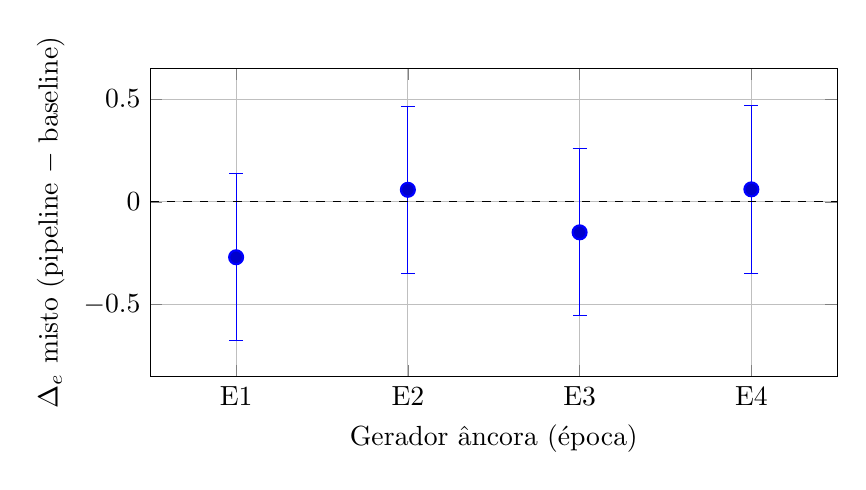
\begin{tikzpicture}
\begin{axis}[
 width=0.85\textwidth,
 height=5.5cm,
 ymin=-0.85, ymax=0.65,
 xmin=0.5, xmax=4.5,
 xtick={1,2,3,4},
 xticklabels={E1,E2,E3,E4},
 ylabel={$\Delta_e$ misto (pipeline $-$ baseline)},
 xlabel={Gerador âncora (época)},
 grid=major,
]
\addplot+[
  only marks,
  mark=*,
  mark size=2.5pt,
  thick,
  error bars/.cd,
  y dir=both,
  y explicit,
] coordinates {
 (1,-0.269) +- (0,0.406)
 (2, 0.059) +- (0,0.405)
 (3,-0.148) +- (0,0.406)
 (4, 0.061) +- (0,0.409)
};
\draw[dashed] (axis cs:0.5,0) -- (axis cs:4.5,0);
\end{axis}
\end{tikzpicture}
\caption{Contrastes \(\Delta_e\) do modelo misto cruzado (filtro estrito), com barras de erro \acrshort{ic}\,95\%. Todos os intervalos incluem zero.}
\label{fig:delta_epoca}
\end{figure}

A Figura~\ref{fig:means_epoca} mostra o padrão mais estável desta amostra: a variação grande está entre geradores âncora, não entre a \textit{baseline} e a condição com sinal.

\begin{figure}[ht]
\centering
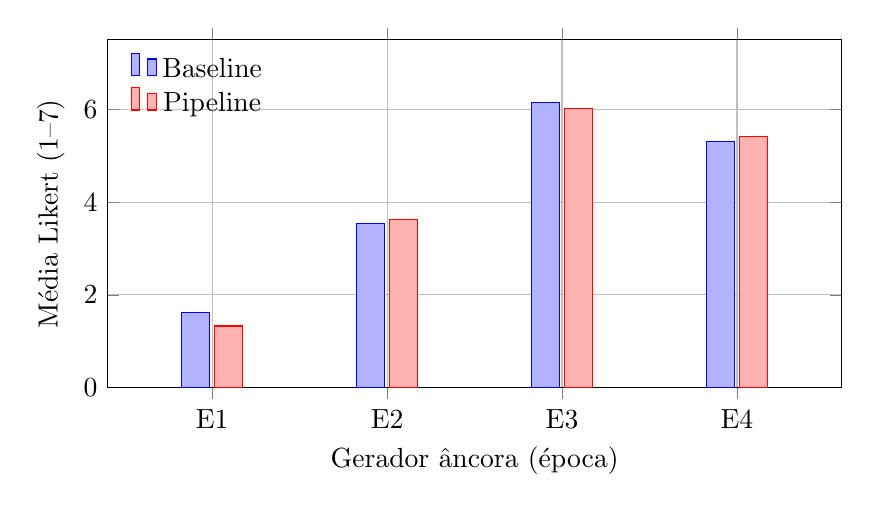
\begin{tikzpicture}
\begin{axis}[
 width=0.9\textwidth,
 height=6cm,
 ybar,
 bar width=10pt,
 ymin=0, ymax=7.5,
 ylabel={Média Likert (1--7)},
 xlabel={Gerador âncora (época)},
 symbolic x coords={E1,E2,E3,E4},
 xtick=data,
 legend style={at={(0.02,0.98)}, anchor=north west, draw=none, fill=none},
 grid=major,
 enlarge x limits=0.2,
]
\addplot coordinates {(E1,1.62) (E2,3.53) (E3,6.15) (E4,5.30)};
\addplot coordinates {(E1,1.33) (E2,3.63) (E3,6.01) (E4,5.41)};
\legend{Baseline, Pipeline}
\end{axis}
\end{tikzpicture}
\caption{Médias absolutas de empatia percebida por época e condição (análise filtro estrito).}
\label{fig:means_epoca}
\end{figure}

%----------------------------------------------------------------------------------------

\section{Inferência principal: modelo misto cruzado}
\label{subsec:res_misto}

Como cada classificação pertence simultaneamente a um participante e a um item, e os mesmos itens são avaliados por vários participantes, estimou-se um modelo linear misto com efeitos aleatórios cruzados de participante e de item (grupo dummy constante e componentes de variância para cada factor) \parencite{Baayen2008Mixed}, sobre o filtro estrito (\(n=2016\); 52 participantes; 96 itens). O output está arquivado em \path{appendices/data/mixed_crossed_strict.json}.

No modelo aditivo \(\textit{score} \sim \textit{condição} + \textit{época}\), a estimativa global da \gls{condicaopipeline} é próxima de zero e não estatisticamente convincente (\(\hat\beta \approx -0{,}07\); \(p \approx 0{,}47\); \gls{ic}\,95\% \([-0{,}28;\,0{,}13]\)), enquanto os coeficientes das épocas E2--E4 face a E1 são grandes e significativos, confirmando que a variação maior está entre geradores âncora.

No modelo com interacção \(\textit{condição}\times\textit{época}\), o teste omnibus da interacção não rejeita a homogeneidade do efeito da condição entre épocas (\(\chi^2(3) \approx 1{,}84\); \(p \approx 0{,}61\)). Os contrastes marginais da condição com sinal face à baseline (Tabela~\ref{tab:misto_contrastes}) incluem zero em todas as âncoras, e nenhum contraste isolado é estatisticamente convincente após o ajuste cruzado.

\begin{table}[ht]
\centering
\caption[Contrastes do modelo misto cruzado.]{Contrastes da condição com sinal face à baseline do modelo misto cruzado (filtro estrito; \acrshort{reml}), com \acrshort{se} e \acrshort{ic}\,95\%.}
\label{tab:misto_contrastes}
\begin{tabular}{lcccc}
\hline
Época & \(\Delta\) & \acrshort{se} & \(p\) & \acrshort{ic}\,95\% \\
\hline
E1 & $-0{,}27$ & 0{,}21 & 0{,}19 & $[-0{,}68;\,0{,}14]$ \\
E2 & $+0{,}06$ & 0{,}21 & 0{,}78 & $[-0{,}35;\,0{,}46]$ \\
E3 & $-0{,}15$ & 0{,}21 & 0{,}48 & $[-0{,}55;\,0{,}26]$ \\
E4 & $+0{,}06$ & 0{,}21 & 0{,}77 & $[-0{,}35;\,0{,}47]$ \\
\hline
\end{tabular}
\end{table}

Não se detectou um efeito estatisticamente convincente da condição na análise hierárquica principal: não se encontra benefício detectável do sinal de ambivalência em nenhuma âncora, nem prejuízo robusto em E1. Esse resultado, face às grandes diferenças absolutas entre geradores, é o achado central deste capítulo.

\subsection{Análises de sensibilidade}
\label{subsec:res_sensibilidade}

No filtro \textit{atenção} (56 participantes; 2112 classificações, sem exclusão por ritmo), os \(\Delta\) descritivos mantêm a mesma direcção geral: E1 \(-0{,}28\) (Welch \(p \approx 0{,}007\)), E2 \(+0{,}08\) (\(p \approx 0{,}60\)), E3 \(-0{,}21\) (\(p \approx 0{,}023\)), E4 \(+0{,}04\) (\(p \approx 0{,}76\)). Em E3, o contraste Welch torna-se significativo quando se incluem os quatro participantes de ritmo rápido, mas trata-se de uma descrição suplementar, não do resultado principal.

Com todas as 2500 classificações com item e pontuação no export (\textit{todos}; o ficheiro bruto tem 2561 linhas, 61 sem célula válida), os \(\Delta\) descritivos são E1 \(-0{,}26\), E2 \(+0{,}15\), E3 \(-0{,}16\), E4 \(0{,}00\). Como quase todas as classificações vêm de sessões concluídas com atenção correcta, este recorte acrescenta pouca informação e não deve ser lido como demonstração formal de robustez.

Com peso igual por participante (média das médias por pessoa, em vez de pooling de classificações), os \(\Delta\) são E1 \(-0{,}52\), E2 \(+0{,}08\), E3 \(-0{,}11\), E4 \(-0{,}18\). A direcção em E1 agrava-se sob equalização, o que é compatível com a influência dos participantes com maior volume nas médias pooled, e mesmo assim, o misto cruzado (que já modela participante e item) permanece a inferência principal e não estabelece um efeito convincente.

O item de prática efectivo, com \texttt{practice\_item\_id} nulo na configuração, é o primeiro do catálogo importado: \texttt{s01\_\_E1\_\_baseline}. Na análise estrita, 25 participantes voltaram a avaliar essa célula na rotação (uma vez cada). Excluindo essas 25 classificações, o \(\Delta\) descritivo de E1 passa a \(-0{,}36\) (Welch); E2--E4 quase não mudam. A prática pode ancorar a escala e reaparecer no bloco pontuado, e recomenda-se, em trabalho futuro, um item neutro dedicado que nunca reentre na amostra.

%----------------------------------------------------------------------------------------

\section{Discussão}
\label{sec:res_discussao}

A hipótese do Capítulo~\ref{chap:Chapter1} previa um \(\Delta\) maior nas âncoras anteriores e residual, ou nulo, nas recentes. Nesta amostra essa forma monotónica não se confirma. Na análise principal, a interacção condição \(\times\) época não foi estatisticamente convincente (\(\chi^2(3) \approx 1{,}84\); \(p \approx 0{,}61\)). No modelo aditivo, o efeito global da \gls{condicaopipeline} foi \(\hat\beta \approx -0{,}07\) (\gls{ic}\,95\% \([-0{,}28;\,0{,}13]\); \(p \approx 0{,}47\)), e todos os contrastes marginais por época apresentaram intervalos de confiança que incluem zero. Não se encontrou evidência do padrão previsto de ganho mais elevado nas âncoras anteriores e residual nas recentes. Estes resultados não demonstram equivalência entre condições; nesta amostra, não há evidência convincente de benefício incremental. A não confirmação da hipótese constitui, por si só, um resultado empírico válido. Não ocorreu o padrão ``ganho claro em DialoGPT e BlenderBot, a cair até zero em Phi-3 e Qwen''. O que se observa, de forma estável, é a diferença entre geradores âncora nas médias absolutas (Figura~\ref{fig:means_epoca}) e um \(\Delta\) do misto cruzado próximo de zero em todas as épocas (Figura~\ref{fig:delta_epoca}), com todos os \gls{ic}\,95\% a incluir zero.

Entre os quatro geradores, as diferenças absolutas entre geradores âncora foram maiores do que as diferenças entre a \gls{baseline} e a condição com sinal. Essas diferenças absolutas misturam arquitectura, alinhamento, tamanho, formato de \textit{prompt} e, como ficou no Capítulo~\ref{chap:Chapter4}, a estratégia de descodificação (gulosa nas âncoras E2--E4; \textit{beam search} no DialoGPT), com temperatura nula nas 96 células. Não devem ser lidas como efeito causal da ``época'' isolada.

\subsection{Leitura por âncora}
\label{subsec:disc_ancoras}

Em E1 o \(\Delta\) descritivo é negativo (\(1{,}62\) versus \(1{,}33\)). O DialoGPT produz respostas curtas e, na \gls{condicaopipeline}, por vezes ecoa os rótulos (``I'm scared and excited'') em vez de os usar como fundo. Uma leitura plausível é que o modelo não sabe incorporar metadados afectivos, ou que o \textit{prompt} extra perturba uma geração já limitada. No misto cruzado o mesmo contraste deixa de ser convincente (\(\Delta \approx -0{,}27\); \(p \approx 0{,}19\); \gls{ic} inclui zero). O \(\Delta\) negativo em E1 fica como leitura descritiva, não como efeito confirmado.

Em E2 o \(\Delta\) descritivo é positivo, como em E4 (\(3{,}53\) versus \(3{,}63\)). É pequeno, o \(d\) de Cohen é \(0{,}06\), e o misto dá \(\approx +0{,}06\) com \(p \approx 0{,}78\). Não há evidência suficiente para concluir benefício. Interpretar este resultado como confirmação da hipótese original seria excessivo.

E3 concentra as notas mais altas. A \gls{baseline} situa-se em \(6{,}15\), perto do topo da escala de sete pontos. Há pouco espaço para a \gls{condicaopipeline} ganhar, e dimensões distintas (validação, compreensão, exploração; aconselhamento, nesta leitura) ficam agregadas num único número \parencite{Kumar2026EmpathicJudging, Sharma2020Empathy, Son2026EmotionalValidation}. Um efeito de tecto ajuda a perceber por que um ganho seria difícil de observar. Não explica, por si, um \(\Delta\) descritivo negativo. As respostas da \gls{condicaopipeline} em E3 tendem ainda a ser mais curtas do que as da \gls{baseline} (cerca de 50 versus 63 palavras, em média, nas 24 células de E3), o que pode contribuir para uma percepção de menor riqueza sem provar causalidade.

E4 impede uma narrativa histórica simples. É a âncora mais recente e a empatia absoluta fica abaixo de E3 (\(5{,}30\) / \(5{,}41\) contra \(6{,}15\) / \(6{,}01\)). Os próprios dados falsificam a leitura ``mais recente, portanto mais empático''. O que varia é o pacote modelo, arquitectura, treino, alinhamento, \textit{prompt} e descodificação. ``Época'' é um agrupador descritivo.

\subsection{O que foi testado, e o que não foi}
\label{subsec:disc_incremental}

A diferença nas médias absolutas, aproximadamente \(1{,}5\) em E1, \(3{,}6\) em E2, \(6{,}1\) em E3 e \(5{,}4\) em E4, é o resultado mais estável desta amostra. Avaliações contemporâneas mostram que respostas de \glspl{llm} avançados podem receber notas muito elevadas de empatia, inclusive comparáveis ou superiores a respostas humanas em determinados desenhos \parencite{Welivita2026HumansOrLLMs, Zhou2026TextEmotionEmpathy}. Nesta amostra, o gerador âncora associa-se a muito mais variação na empatia percebida do que o sinal de ambivalência. Isso é compatível com um baseline comunicativo já forte nos modelos \textit{instruct}.

Este estudo não testou se a ambivalência emocional ``importa''. Testou algo mais estreito: se adicionar ao gerador um sinal de ambivalência derivado do \textit{mesmo} enunciado produz empatia percebida incremental face ao enunciado sozinho. A resposta encontrada é que, nesta amostra, não de forma consistente.

Isto não autoriza concluir que condicionamento emocional por \textit{prompt} seja inútil em \glspl{llm} modernos. Dong e colaboradores mostram que GPT-4, sem \textit{prompting} específico, ainda ficava abaixo de conselheiros humanos em suporte emocional, e que \textit{prompts} fundamentados em teoria e competências de ajuda melhoravam consideravelmente o desempenho \parencite{Dong2025GPT4EmotionSupport}. Bieberstein e colaboradores, num estudo controlado com o mesmo \gls{llm} e só a instrução de sistema a mudar (neutra versus explicitamente empática), encontram diferenças de empatia percebida pequenas e inconclusivas, e levantam a hipótese de que modelos alinhados já trazem um baseline prosocial que reduz o contraste de instruções extra \parencite{Bieberstein2026PromptEmpathy}. O contraste é útil para E3 e E4: prompting estruturado pode ajudar em alguns contextos, mas instruções afectivas acrescentadas a um modelo já alinhado podem não criar diferença perceptível. A explicitação de rótulos afectivos derivados do próprio enunciado não apresentou benefício incremental detectável neste desenho.

\subsection{Interferência, granularidade e o que vem depois do rótulo}
\label{subsec:disc_mecanismos}

Uma hipótese interpretativa para o \(\Delta\) descritivo negativo em E3 vem das críticas a pipelines centradas no rótulo emocional: informação afectiva reconhecida pode conflitar com o contexto que o modelo já extrai do enunciado, empurrando a geração para respostas mais genéricas \parencite{Huangfu2025NEC}. O sinal não seria apenas redundante, e em alguns casos poderia interferir numa representação mais rica construída directamente a partir do enunciado. Trata-se de uma hipótese, não de um mecanismo demonstrado por este experimento. Evidência independente, noutro regime, mostra que intervenções pensadas para aumentar calor ou validação podem alterar outras propriedades da geração. Ibrahim, Hafner e Rocher encontram que treinar modelos para respostas mais ``quentes'' reduz exactidão factual e aumenta sycophancy \parencite{Ibrahim2026WarmSycophancy}. Esse trabalho usa \textit{fine-tuning} e mede desfechos diferentes dos desta dissertação, e não explica o \(\Delta\) de E3. O ponto útil é que uma intervenção afectiva não é, por omissão, uma operação neutra.

Uma leitura complementar centra-se na granularidade. Trabalhos de recuperação guiada por similaridade emocional, como o \gls{reg}, sugerem que atributos afectivos podem ajudar a orientar a geração, mas identificam ruído e baixa diversidade quando se trabalha com atributos grosseiros ao nível da sentença \parencite{Wang2026REG}. Reduzir um enunciado emocionalmente rico a dois rótulos relativamente grosseiros pode, assim, constituir uma compressão pobre. O problema talvez não seja fornecer informação emocional, mas a granularidade da informação fornecida. Modelos que representam emoções mistas e a sua dinâmica ao longo do diálogo, como o \gls{mege}, encontram benefício precisamente ao estruturar essa complexidade no processo de geração, e não ao inserir apenas dois rótulos no \textit{prompt} \parencite{Zhao2026MEGE}. Distinguir ``esta operacionalização não trouxe benefício detectável'' de ``modelar ambivalência não traz benefício'' é essencial para não sobreinterpretar o \(\Delta\).

Noutra linha, a \gls{condicaopipeline} acrescenta sobretudo uma descrição emocional do enunciado, enquanto a literatura recente reporta benefícios ao acrescentar estrutura causal e inferencial, raciocínio sobre causas, desejos e intenções antes de responder \parencite{Fu2023ReasoningBeforeResponding, Chen2024CauseAware, He2025ECC}. Uma frase do tipo ``joy + fear'' pode não gerar ganho mesmo que informação afectiva mais elaborada ainda seja útil. Mesmo compreender a emoção e a sua causa pode não bastar: o sistema precisa de decidir que resposta é requerida. Frameworks centrados na intenção de suporte e trabalhos sobre validação emocional sublinham que a empatia percebida depende, em grande medida, da adequação pragmática da estratégia, validar, explorar, perguntar ou aconselhar, e não apenas da precisão do rótulo \parencite{Zhang2025IntentionESC, Son2026EmotionalValidation, Wan2025EmoDynamiX}.

\subsection{Validade de constructo da ambivalência}
\label{subsec:disc_constructo}

A avaliação humana valida a empatia das \textit{respostas}, não se o GoEmotions coincide com a ambivalência percebida. O mesmo classificador define o que conta como ambivalente, filtra os 12 estímulos e fornece o sinal injectado \parencite{Demszky2020GoEmotions}. Dois rótulos não preservam intensidade, dominância nem tensão \parencite{Singh2026MultiEmotionIntensity}.

Esta ameaça impede distinguir pelo menos três explicações do resultado. O sinal pode representar bem a ambivalência e ser redundante para o gerador. Pode representá-la bem e o gerador não a converter numa estratégia mais empática. Pode não corresponder suficientemente à ambivalência percebida por humanos. O desenho avalia só o efeito final sobre a empatia percebida e não separa estes mecanismos. A ausência de benefício detectável da condição não é evidência de que a ambivalência seja irrelevante. É ausência de benefício detectável desta operacionalização.

\subsection{Poder estatístico e implicação prática}
\label{subsec:disc_poder}

Os erros-padrão do misto cruzado rondam \(0{,}21\) pontos Likert. Os \gls{ic} a 95\% têm largura próxima de \(0{,}8\) pontos: em E1, \([-0{,}68;\,0{,}14]\); em E3, \([-0{,}55;\,0{,}26]\). Diferenças pequenas da condição, da ordem de \(0{,}1\) a \(0{,}2\) pontos, cabem folgadamente nesses intervalos. Não detectar um contraste estatisticamente convincente não demonstra equivalência entre a condição com sinal e a baseline. A conclusão correcta é mais estreita: nesta amostra, não se encontrou evidência convincente de benefício incremental.

Mesmo que um \(\Delta\) de \(+0{,}1\) viesse a tornar-se significativo com milhares de classificações, a pergunta prática para quem desenha chatbots continua de pé. Vale a complexidade de um classificador, uma regra de ambivalência e um \textit{prompt} extra por um décimo de ponto numa escala de sete? Nesta operacionalização, e com médias já altas em E3, o ganho perceptivo esperado é pequeno. Isso não diz que informação afectiva seja inútil.

Por fim, uma resposta isolada com nota elevada não demonstra compreensão empática longitudinal. Avaliações que observam mudanças emocionais ao longo do diálogo procuram capturar outra coisa \parencite{Zhang2026SAGE}. Esta observação liga a discussão às limitações e ao trabalho futuro do Capítulo~\ref{chap:Chapter6}.

%----------------------------------------------------------------------------------------

% Chapter 6
% Conclusões e Trabalho Futuro

\chapter{Conclusões e Trabalho Futuro}
\label{chap:Chapter6}

Este capítulo sintetiza as conclusões empíricas do Capítulo~\ref{chap:Chapter5}, as limitações e o trabalho futuro.

%----------------------------------------------------------------------------------------

\section{Síntese dos contributos}
\label{sec:conc_contributos}

O trabalho produziu os seguintes contributos: (i) uma definição operacional de \gls{ambivalenciaemocional} a partir da classificação multilabel GoEmotions; (ii) uma \gls{pipeline} documentada e disponibilizada para replicação, em Python, com Hugging Face Transformers, que injecta esse sinal no contexto de geração; (iii) um protocolo cego factorial (condição \(\times\) época) com quatro geradores âncora alinhados a marcos históricos; (iv) um questionário online desenvolvido para este estudo e uma análise centrada no diferencial \(\Delta\) e nas médias absolutas de empatia percebida. As 96 células foram geradas, e a avaliação humana, com 52 participantes no filtro estrito e 2016 classificações na análise principal, está reportada no Capítulo~\ref{chap:Chapter5}.

%----------------------------------------------------------------------------------------

\section{Conclusões}
\label{sec:conc_conclusoes}

Foi construída uma definição operacional de ambivalência a partir do GoEmotions, uma pipeline em Python, com Hugging Face Transformers, que injecta esse sinal no contexto de geração, e um questionário cego com 96 células. Foi testado se esse sinal, face a uma \gls{baseline} sem metadados, aumenta a empatia percebida em quatro geradores âncora.

A hipótese não se confirma. Os quatro contrastes da condição com sinal face à baseline, no modelo misto cruzado, incluem zero no \gls{ic}\,95\% (Tabela~\ref{tab:misto_contrastes}). A variação está entre geradores âncora, cerca de \(1{,}5\) em E1 e cerca de \(6{,}1\) em E3. A pipeline foi implementada e executada com sucesso, permitindo operacionalizar e tornar explícito o sinal de ambivalência; contudo, a sua utilização não produziu melhoria consistente da empatia percebida.

O resultado sustenta apenas que a explicitação de rótulos afectivos derivados do próprio enunciado não apresentou valor incremental detectável neste desenho; não demonstra equivalência entre condições, porque os intervalos de confiança são largos para efeitos pequenos, nem inutilidade da informação afectiva. A interpretação permanece limitada pela ausência de validação humana da ambivalência (Secção~\ref{subsec:disc_constructo}).

O passo seguinte, desenvolvido na Secção~\ref{sec:conc_futuro}, é validar humanamente a detecção de ambivalência, e não repetir o mesmo desenho com mais participantes.

%----------------------------------------------------------------------------------------

\section{Limitações}
\label{sec:conc_limitacoes}

A principal ameaça à validade de constructo decorre da dependência de um único classificador e limiar para definir, seleccionar e representar a ambivalência (Secção~\ref{subsec:disc_constructo}).

As diferenças entre âncoras confundem época, modelo e descodificação; a «época» não foi isolada (Capítulos~\ref{chap:Chapter4} e~\ref{chap:Chapter5}). Uma só resposta por estímulo \(\times\) gerador \(\times\) condição não estima a variabilidade entre outputs do mesmo gerador âncora.

A amostra é de conveniência, por bola de neve na rede pessoal e académica. Iniciaram 156 pessoas; concluíram 63; o filtro estrito retém 52. O abandono é sobretudo precoce. Sem demografia, não se testa se completadores e desistentes diferem. A tradução automática EN\(\rightarrow\)PT foi revista por humano. As respostas dos geradores âncora tiveram apenas uma revisão mínima, alinhada à \gls{qa} automática: células recusadas voltaram a ser executadas na mesma célula até a \gls{qa} aceitar, sem editar o texto nem escolher entre várias válidas. O número de células regeneradas não ficou registado no log. O conteúdo restante não foi editado, para preservar o comportamento gerado.

A cegagem reduz enviesamentos de expectativa, mas não tira a subjectividade da empatia percebida. A opção de itens extra após o mínimo introduz auto-selecção no volume (mediana 24 itens; sete participantes avaliaram as 96 células). O item de prática (\texttt{s01\_\_E1\_\_baseline}) pode reaparecer na rotação pontuada. O ritmo demasiado rápido excluiu quatro participantes no filtro estrito. A verificação de atenção usa um alvo fixo (valor 2). Os testes Welch ao nível da classificação são apenas suplementares; a inferência principal é o misto cruzado (Secção~\ref{subsec:disc_poder}).

A medida de empatia é uma escala global de sete pontos. A escala ordinal foi modelada como contínua na análise principal, por meio de um modelo misto linear, opção comum em escalas de sete pontos com volume elevado de observações; uma replicação poderia verificar robustez com modelos ordinais mistos. Quando as respostas já se situam perto do topo da escala, como em E3 (Secção~\ref{subsec:disc_ancoras}), a sensibilidade a ganhos adicionais diminui. Fala-se aqui em potencial efeito de tecto observado nesta amostra. O desenho avalia respostas isoladas a enunciados isolados. Uma nota elevada num único enunciado não equivale a compreensão social longitudinal \parencite{Zhang2026SAGE}.

A escolha do endpoint, juízo humano cego, e não um modelo a classificar empatia, é uma força do desenho. Comparações recentes entre juízes-\gls{llm} e especialistas encontram inflação nas notas automáticas e menor fiabilidade em dimensões afectivas \parencite{Badawi2026MentalAlign}. Essa força não compensa as ameaças acima; apenas evita uma fonte adicional de viés no critério.

%----------------------------------------------------------------------------------------

\section{Trabalho futuro}
\label{sec:conc_futuro}

O passo que os resultados desta dissertação justificam de forma mais directa é uma validação humana da detecção de ambivalência, independente da geração. Avaliadores, nos mesmos 12 estímulos e antes de qualquer geração, identificam as emoções percebidas, classificam a intensidade de cada uma e avaliam o grau de ambivalência do enunciado. Estima-se a concordância entre avaliadores e entre os juízos humanos e o GoEmotions. Índices como o \(\alpha\) de Krippendorff ou o coeficiente de correlação intraclasse (ICC) ficam como possibilidade, não como método fixo. Sem isso, um \(\Delta\) próximo de zero mistura ``esta operacionalização não teve benefício detectável'' com ``o sinal não mede o constructo''. Qualquer extensão da pipeline deve esperar por essa validação.

Com estímulos assim validados, uma replicação controlada poderia incluir textos não ambivalentes como controlo, várias gerações por célula com parâmetros uniformes, uma escala multi-item de empatia e verificação ordinal de robustez. Extensões como mais âncoras, outras línguas ou variação de \(\tau\) só fazem sentido depois deste controlo.

O resultado observado sugere que o valor, se existir, está menos em explicitar rótulos derivados do próprio enunciado e mais numa representação intermédia (causa, necessidade e estratégia de resposta), a testar só depois da validação humana e da replicação controlada.

Num horizonte posterior, poderá também avaliar-se se histórico conversacional e informação personalizada acrescentam valor que não está disponível no enunciado isolado.

%----------------------------------------------------------------------------------------


%----------------------------------------------------------------------------------------
%	GLOSSARY
%----------------------------------------------------------------------------------------

\printglossary[title={Glossário},style=altlist]

%----------------------------------------------------------------------------------------
%	BIBLIOGRAPHY
%----------------------------------------------------------------------------------------

\printbibliography[heading=bibintoc,title={Referências}]

%----------------------------------------------------------------------------------------
%	THESIS CONTENT - APPENDICES
%----------------------------------------------------------------------------------------
% Include the appendices of the thesis as separate files from the Appendices folder
% Uncomment the lines as you write the Appendices
\begin{appendices}

% Appendix A

\chapter{Materiais experimentais}
\label{AppendixA}

\section{Estímulos (inglês)}

Os doze estímulos utilizados no estudo principal (ficheiros \texttt{stimuli.json} da pipeline) são:

\begin{enumerate}
 \item \textit{I am so proud and happy about this promotion, but I am also scared and anxious that everyone will soon see that I do not deserve it.}
 \item \textit{I'm genuinely happy for my sister's wedding, yet I also feel lonely and left behind in my own life.}
 \item \textit{I love living in this city and all the opportunities here, but the rent stress is making me resent every morning.}
 \item \textit{I'm proud that I finished the marathon, although my injury still scares me and I keep thinking I pushed too hard.}
 \item \textit{I want to start this new relationship because I care about them, but I also feel anxious that I will get hurt again.}
 \item \textit{I'm grateful my parents support me financially, yet I feel ashamed and angry that I still depend on them at my age.}
 \item \textit{I feel relieved and even joyful that I finally submitted my thesis, but I am also disappointed and worried because parts of it are still weak.}
 \item \textit{I'm excited about moving abroad for work, while at the same time I feel sad about leaving my friends and family.}
 \item \textit{I admire my colleague's confidence in meetings, but I also feel annoyed and small whenever they interrupt me.}
 \item \textit{I'm hopeful the medical results will be fine, yet every notification on my phone fills me with dread.}
 \item \textit{I enjoy remote work and the freedom it gives me, but I miss the office and feel disconnected from the team.}
 \item \textit{I'm glad I told the truth in that argument, although I regret how harsh I sounded and keep replaying it.}
\end{enumerate}

Apenas estímulos classificados como ambivalentes pelo GoEmotions com \(\tau = 0{,}10\) entram no lote de geração.

\section{Identificadores Hugging Face}

\begin{itemize}
 \item Classificador: \texttt{SamLowe/roberta-base-go\_emotions}
 \item E1: \texttt{microsoft/DialoGPT-medium}
 \item E2: \texttt{facebook/blenderbot-400M-distill}
 \item E3: \texttt{microsoft/Phi-3-mini-4k-instruct}
 \item E4: \texttt{Qwen/Qwen2.5-3B-Instruct}
\end{itemize}

\section{Consentimento e instrução ao avaliador}

O instrumento de recolha foi um questionário online bilingue (português e inglês), desenvolvido para este estudo. Capturas da interface do participante e do painel de administração constam do Capítulo~\ref{chap:Chapter4}. O texto de consentimento informado e a instrução Likert (empatia 1--7) eram apresentados na interface, antes e durante a avaliação. Em síntese, os participantes adultos (\(\ge 18\) anos) avaliam respostas sem conhecer o modelo nem a condição experimental, após consentimento voluntário, e não se pedem dados demográficos. Após cerca de 24 itens, podem optar por continuar com itens adicionais ou concluir, seguindo-se uma verificação de atenção.

% Auto-generated by export_appendix_responses.py --- do not edit by hand
\chapter{Respostas geradas (baseline vs condição com sinal)}
\label{AppendixB}

As respostas reproduzidas neste apêndice são outputs experimentais dos
modelos avaliados e não constituem texto autoral da dissertação.
Este apêndice apresenta as respostas geradas pela pipeline experimental,
organizadas por estímulo. Para cada estímulo indica-se o enunciado de
entrada e o par de emoções dominantes (positiva e negativa) obtido pelo
classificador GoEmotions, o mesmo sinal injectado na condição com sinal
(codificada como \textit{pipeline} nos dados). Seguem-se, por época, as respostas
\textit{baseline} (sem sinal) e da condição com sinal.
O ficheiro-fonte completo encontra-se em
\path{appendices/data/all_results.json}.

Total de células incluídas: 96.

\section{Estímulo \texttt{s01}}
\textit{I am so proud and happy about this promotion, but I am also scared and anxious that everyone will soon see that I do not deserve it.}

Ambivalência (GoEmotions): emoção positiva dominante \textit{alegria} (\texttt{joy}); emoção negativa dominante \textit{medo} (\texttt{fear}).

\subsection*{E1: DialoGPT-medium (\texttt{microsoft/DialoGPT-medium})}
\textbf{Baseline:}

I don't think you deserve it.

\textbf{Pipeline:}

I don't deserve it either. I'm scared and excited.

\subsection*{E2: BlenderBot (\texttt{facebook/blenderbot-400M-distill})}
\textbf{Baseline:}

Why do you think you don't deserve it? I'm sure you're doing a great job.

\textbf{Pipeline:}

I'm sure you'll do just fine. Just be confident in yourself and you'll be fine.

\subsection*{E3: Phi-3-mini-Instruct (\texttt{microsoft/Phi-3-mini-4k-instruct})}
\textbf{Baseline:}

It's completely normal to feel a mix of emotions when you receive a promotion. Your hard work and dedication have led to this achievement, and it's a testament to your abilities. Remember, it's okay to have doubts, but try to focus on your accomplishments and the positive impact you've made. You deserve this promotion, and it's important to believe in yourself.

\textbf{Pipeline:}

Congratulations on your promotion! It's natural to feel a mix of emotions during such a significant change. Remember, your hard work and dedication have led you to this moment, and it's okay to take some time to adjust to your new role.

\subsection*{E4: Qwen2.5-3B-Instruct (\texttt{Qwen/Qwen2.5-3B-Instruct})}
\textbf{Baseline:}

It's natural to feel both proud and anxious during a promotion. Remember, your hard work and dedication are what led to this opportunity, and it's okay to feel uncertain about how others perceive it.

\textbf{Pipeline:}

It's understandable to feel both excited and apprehensive about a promotion. Remember, deserving something isn't always about your current abilities but about the growth and effort you've shown.

\section{Estímulo \texttt{s02}}
\textit{I'm genuinely happy for my sister's wedding, yet I also feel lonely and left behind in my own life.}

Ambivalência (GoEmotions): emoção positiva dominante \textit{alegria} (\texttt{joy}); emoção negativa dominante \textit{tristeza} (\texttt{sadness}).

\subsection*{E1: DialoGPT-medium (\texttt{microsoft/DialoGPT-medium})}
\textbf{Baseline:}

I'm sorry for your loss.

\textbf{Pipeline:}

Joyous and sad.

\subsection*{E2: BlenderBot (\texttt{facebook/blenderbot-400M-distill})}
\textbf{Baseline:}

I'm sorry to hear that. Have you talked to her about how you feel about it?

\textbf{Pipeline:}

I'm sorry to hear that. I'm sure your sister is happy for you as well.

\subsection*{E3: Phi-3-mini-Instruct (\texttt{microsoft/Phi-3-mini-4k-instruct})}
\textbf{Baseline:}

I'm glad to hear that you're happy for your sister's wedding; it's a special occasion. It's completely normal to feel a bit of loneliness during such times, especially when life seems to be moving forward for others. Remember, it's okay to take a moment for yourself and reflect on your own journey. Perhaps this could be a time to focus on personal growth or to reach out to friends and family for support.

\textbf{Pipeline:}

It's wonderful to hear that you're celebrating your sister's wedding and are happy for her. It's natural to feel a mix of emotions during such significant events. Perhaps you could find comfort in sharing your feelings with friends or family, or even consider planning a special day for yourself to reflect and enjoy.

\subsection*{E4: Qwen2.5-3B-Instruct (\texttt{Qwen/Qwen2.5-3B-Instruct})}
\textbf{Baseline:}

It's common to feel a mix of emotions during such joyous occasions. Perhaps focusing on your own happiness and well-being can help balance those feelings.

\textbf{Pipeline:}

I understand that your sister's wedding is a joyous occasion, but it's also natural to feel a bit left out sometimes. How about you reach out to friends or family members who might be able to offer some companionship during this time?

\section{Estímulo \texttt{s03}}
\textit{I love living in this city and all the opportunities here, but the rent stress is making me resent every morning.}

Ambivalência (GoEmotions): emoção positiva dominante \textit{amor} (\texttt{love}); emoção negativa dominante \textit{tristeza} (\texttt{sadness}).

\subsection*{E1: DialoGPT-medium (\texttt{microsoft/DialoGPT-medium})}
\textbf{Baseline:}

I like your username though.

\textbf{Pipeline:}

Love, sadness, etc. I love the user's attitude.

\subsection*{E2: BlenderBot (\texttt{facebook/blenderbot-400M-distill})}
\textbf{Baseline:}

I'm sorry to hear that. Is there anything you can do to make it less stressful?

\textbf{Pipeline:}

I'm sorry to hear that. Do you have any hobbies to take your mind off of it?

\subsection*{E3: Phi-3-mini-Instruct (\texttt{microsoft/Phi-3-mini-4k-instruct})}
\textbf{Baseline:}

I'm sorry to hear that you're feeling stressed about rent. It's important to find a balance between enjoying your city and managing your finances. Have you considered looking for a roommate or exploring more affordable neighborhoods? Sometimes, small changes can make a big difference in your daily life.

\textbf{Pipeline:}

I'm sorry to hear that you're feeling stressed about the rent. It's great to hear that you love living in the city and appreciate the opportunities it offers. Have you considered looking into more affordable housing options or perhaps speaking with a financial advisor to help manage your expenses?

\subsection*{E4: Qwen2.5-3B-Instruct (\texttt{Qwen/Qwen2.5-3B-Instruct})}
\textbf{Baseline:}

It's understandable that the rent stress can affect your mood, but remember to prioritize self-care and possibly explore if there are any local resources or support groups that can help manage your financial stress.

\textbf{Pipeline:}

I understand that the love you have for your city is strong, but the rent stress can definitely make mornings feel tough. How about exploring any potential ways to reduce your expenses or find more affordable housing options?

\section{Estímulo \texttt{s04}}
\textit{I'm proud that I finished the marathon, although my injury still scares me and I keep thinking I pushed too hard.}

Ambivalência (GoEmotions): emoção positiva dominante \textit{alegria} (\texttt{joy}); emoção negativa dominante \textit{medo} (\texttt{fear}).

\subsection*{E1: DialoGPT-medium (\texttt{microsoft/DialoGPT-medium})}
\textbf{Baseline:}

I don't know what to tell you.

\textbf{Pipeline:}

Joyousness and fear. I'm not sure what's going on.

\subsection*{E2: BlenderBot (\texttt{facebook/blenderbot-400M-distill})}
\textbf{Baseline:}

How long did it take you to finish it? I'm sure you did great though.

\textbf{Pipeline:}

You should be proud of yourself. It takes a lot of courage to do something like that.

\subsection*{E3: Phi-3-mini-Instruct (\texttt{microsoft/Phi-3-mini-4k-instruct})}
\textbf{Baseline:}

It's truly commendable that you completed the marathon despite your injury. Remember, it's important to listen to your body and not push beyond your limits. Perhaps consider consulting with a healthcare professional to ensure you're on the right track for recovery. Your determination is admirable, but your health should always come first.

\textbf{Pipeline:}

It's truly commendable that you've completed the marathon; that's a significant achievement. It's natural to feel some apprehension about your injury, but remember that taking care of your health is paramount. Perhaps consider consulting with a healthcare professional to ensure you're on the right track for recovery.

\subsection*{E4: Qwen2.5-3B-Instruct (\texttt{Qwen/Qwen2.5-3B-Instruct})}
\textbf{Baseline:}

It's great to hear that you finished the marathon, even with the lingering concern about pushing too hard and your injury. Recovery is important, so take the time you need to heal properly.

\textbf{Pipeline:}

It's great to hear that you finished the marathon, even with the lingering fear of pushing too hard. How are you managing to cope with those thoughts?

\section{Estímulo \texttt{s05}}
\textit{I want to start this new relationship because I care about them, but I also feel anxious that I will get hurt again.}

Ambivalência (GoEmotions): emoção positiva dominante \textit{desejo} (\texttt{desire}); emoção negativa dominante \textit{nervosismo} (\texttt{nervousness}).

\subsection*{E1: DialoGPT-medium (\texttt{microsoft/DialoGPT-medium})}
\textbf{Baseline:}

I care about you.

\textbf{Pipeline:}

Desire, nervousness, anxiousness, and anxiousness respectively.

\subsection*{E2: BlenderBot (\texttt{facebook/blenderbot-400M-distill})}
\textbf{Baseline:}

Why do you feel that way? Do you think you'll be able to get through it?

\textbf{Pipeline:}

I'm sure you'll be fine. Relationships are hard, but it's worth it in the end.

\subsection*{E3: Phi-3-mini-Instruct (\texttt{microsoft/Phi-3-mini-4k-instruct})}
\textbf{Baseline:}

It's completely normal to feel anxious about getting hurt in a new relationship, especially if you've experienced it before. Remember that taking the risk of opening up to someone new can lead to rewarding connections. It's important to communicate your feelings and concerns with your partner, and to take things at a pace that feels comfortable for you. Building trust and setting healthy boundaries can help you navigate this new relationship with care and mindfulness.

\textbf{Pipeline:}

It's completely normal to feel a mix of emotions when considering a new relationship. It's important to communicate openly with your partner about your feelings and concerns. Taking things slow and building trust can help ease your anxiety. Remember, it's okay to prioritize your emotional well-being.

\subsection*{E4: Qwen2.5-3B-Instruct (\texttt{Qwen/Qwen2.5-3B-Instruct})}
\textbf{Baseline:}

It's natural to feel anxious after past hurt. Honesty with your feelings can help both of you navigate this relationship carefully.

\textbf{Pipeline:}

It's natural to feel both drawn to someone and worried about potential hurt in a new relationship. How can I help you navigate these feelings?

\section{Estímulo \texttt{s06}}
\textit{I'm grateful my parents support me financially, yet I feel ashamed and angry that I still depend on them at my age.}

Ambivalência (GoEmotions): emoção positiva dominante \textit{gratidão} (\texttt{gratitude}); emoção negativa dominante \textit{embaraço} (\texttt{embarrassment}).

\subsection*{E1: DialoGPT-medium (\texttt{microsoft/DialoGPT-medium})}
\textbf{Baseline:}

How do you feel about your parents'financial support?

\textbf{Pipeline:}

Thank you for your feedback. Thanks for your input. Thank you.

\subsection*{E2: BlenderBot (\texttt{facebook/blenderbot-400M-distill})}
\textbf{Baseline:}

I know what you mean. I'm glad my parents are supportive of me as well.

\textbf{Pipeline:}

I know what you mean. I feel the same way. I'm glad my parents are supportive.

\subsection*{E3: Phi-3-mini-Instruct (\texttt{microsoft/Phi-3-mini-4k-instruct})}
\textbf{Baseline:}

It's completely normal to feel a mix of emotions when it comes to financial support from parents. Remember, seeking help is a sign of strength, not weakness. It's important to communicate openly with your parents about your feelings and work together to find a solution that respects your independence while acknowledging their support.

\textbf{Pipeline:}

It's completely normal to feel a mix of emotions when it comes to financial support from family. Remember that it's okay to rely on your parents, and it's a sign of their love and care for you. It's also important to communicate openly with them about your feelings and work together to find a path to financial independence that feels right for you.

\subsection*{E4: Qwen2.5-3B-Instruct (\texttt{Qwen/Qwen2.5-3B-Instruct})}
\textbf{Baseline:}

It's common to feel a mix of emotions about financial dependence, but it's important to recognize that your parents' support is a reflection of their love and care for you. You might consider talking to them about your feelings to find a way to move forward together.

\textbf{Pipeline:}

It's common to feel a mix of emotions when you're still relying on your parents financially. Gratitude for their support is a positive feeling, but the shame and anger you're experiencing are understandable too.

\section{Estímulo \texttt{s07}}
\textit{I feel relieved and even joyful that I finally submitted my thesis, but I am also disappointed and worried because parts of it are still weak.}

Ambivalência (GoEmotions): emoção positiva dominante \textit{alegria} (\texttt{joy}); emoção negativa dominante \textit{nervosismo} (\texttt{nervousness}).

\subsection*{E1: DialoGPT-medium (\texttt{microsoft/DialoGPT-medium})}
\textbf{Baseline:}

I don't know what I'm doing.

\textbf{Pipeline:}

Joyous and nervous. I'm not sure what's going on.

\subsection*{E2: BlenderBot (\texttt{facebook/blenderbot-400M-distill})}
\textbf{Baseline:}

I'm sure you did great! I know how you feel though, it can be nerve wracking.

\textbf{Pipeline:}

I'm sure you did great! I know how you feel though, it can be nerve wracking.

\subsection*{E3: Phi-3-mini-Instruct (\texttt{microsoft/Phi-3-mini-4k-instruct})}
\textbf{Baseline:}

I'm glad to hear that you've submitted your thesis and are feeling relieved and joyful about this accomplishment. It's completely normal to have mixed feelings after such a significant milestone. Remember, it's okay to feel disappointed and worried about the parts that need improvement. This is a great opportunity to refine your work and strengthen your arguments. Keep focusing on the positive progress you've made, and don't hesitate to seek feedback to enhance your thesis further.

\textbf{Pipeline:}

I'm really proud of you for submitting your thesis! It's a significant accomplishment, and it's normal to feel a mix of emotions. Remember, it's okay to take some time to review and strengthen the parts you're not as confident about. You've got this!

\subsection*{E4: Qwen2.5-3B-Instruct (\texttt{Qwen/Qwen2.5-3B-Instruct})}
\textbf{Baseline:}

It's great to hear you feel relieved and joyful about submitting your thesis. It's natural to feel disappointed and worried about the areas that need improvement, but remember, this is a normal part of the process.

\textbf{Pipeline:}

It's great to hear that you feel relieved and joyful about submitting your thesis. However, it's understandable to feel a bit nervous and disappointed about the parts that still need improvement.

\section{Estímulo \texttt{s08}}
\textit{I'm excited about moving abroad for work, while at the same time I feel sad about leaving my friends and family.}

Ambivalência (GoEmotions): emoção positiva dominante \textit{excitação} (\texttt{excitement}); emoção negativa dominante \textit{tristeza} (\texttt{sadness}).

\subsection*{E1: DialoGPT-medium (\texttt{microsoft/DialoGPT-medium})}
\textbf{Baseline:}

I don't know what to do with my life.

\textbf{Pipeline:}

I don't know what to do with my hands!!!

\subsection*{E2: BlenderBot (\texttt{facebook/blenderbot-400M-distill})}
\textbf{Baseline:}

I'm sure you'll make new friends when you get back. Where are you moving to?

\textbf{Pipeline:}

That's understandable. I'm sure you'll make new friends though. Where are you moving to?

\subsection*{E3: Phi-3-mini-Instruct (\texttt{microsoft/Phi-3-mini-4k-instruct})}
\textbf{Baseline:}

It's completely normal to feel a mix of emotions when moving abroad for work. The excitement of new opportunities and experiences can be very compelling, but it's also understandable to feel sad about leaving loved ones behind. Remember to stay connected with your friends and family through regular calls or video chats, and consider planning visits to keep those relationships strong.

\textbf{Pipeline:}

It's completely normal to feel a mix of emotions when facing such a significant life change. It's great that you're excited about the new opportunities that await you abroad. Remember, it's also important to cherish the time you have with your loved ones. Keep in touch with them, and perhaps plan a visit back home soon.

\subsection*{E4: Qwen2.5-3B-Instruct (\texttt{Qwen/Qwen2.5-3B-Instruct})}
\textbf{Baseline:}

It's natural to feel excited about new opportunities while also sad to leave behind loved ones. Balancing these emotions can be challenging, but it's a common experience when making big life changes.

\textbf{Pipeline:}

Moving abroad can be incredibly exciting, but it's also natural to feel sad about leaving behind the people you love. How are you planning to stay connected with your friends and family back home?

\section{Estímulo \texttt{s09}}
\textit{I admire my colleague's confidence in meetings, but I also feel annoyed and small whenever they interrupt me.}

Ambivalência (GoEmotions): emoção positiva dominante \textit{admiração} (\texttt{admiration}); emoção negativa dominante \textit{irritação} (\texttt{annoyance}).

\subsection*{E1: DialoGPT-medium (\texttt{microsoft/DialoGPT-medium})}
\textbf{Baseline:}

I'm with you, I'm not.

\textbf{Pipeline:}

I don't know what to do with my hands!!!

\subsection*{E2: BlenderBot (\texttt{facebook/blenderbot-400M-distill})}
\textbf{Baseline:}

Why do you feel that way? Is it because you are intimidated by them?

\textbf{Pipeline:}

I know what you mean. It's hard not to feel that way sometimes. Have you tried talking to them about it?

\subsection*{E3: Phi-3-mini-Instruct (\texttt{microsoft/Phi-3-mini-4k-instruct})}
\textbf{Baseline:}

I understand that it can be frustrating when someone interrupts you, especially in a professional setting. It's important to remember that everyone has their own communication style, and your colleague's confidence might simply be a part of their personality. Perhaps you could address this issue directly with them in a private conversation, expressing how their interruptions make you feel. This way, you can work together to find a more respectful way to communicate during meetings.

\textbf{Pipeline:}

It's great to hear that you appreciate your colleague's confidence; it's a valuable trait in any professional setting. However, it's important to feel respected and heard during meetings. Perhaps you could suggest a meeting etiquette to the team or speak to your colleague privately about how their interruptions make you feel.

\subsection*{E4: Qwen2.5-3B-Instruct (\texttt{Qwen/Qwen2.5-3B-Instruct})}
\textbf{Baseline:}

It's great that you admire your colleague's confidence, but it's important to address the interruptions as they can make you feel small and disrespected. You might consider politely reminding them of the importance of listening to others as well.

\textbf{Pipeline:}

It sounds like you're in a challenging situation where you respect your colleague's assertiveness but find it frustrating. How about discussing this with your colleague to find a way to balance their confidence with your need for respect and space?

\section{Estímulo \texttt{s10}}
\textit{I'm hopeful the medical results will be fine, yet every notification on my phone fills me with dread.}

Ambivalência (GoEmotions): emoção positiva dominante \textit{optimismo} (\texttt{optimism}); emoção negativa dominante \textit{medo} (\texttt{fear}).

\subsection*{E1: DialoGPT-medium (\texttt{microsoft/DialoGPT-medium})}
\textbf{Baseline:}

I'm sorry to hear that.

\textbf{Pipeline:}

I don't know what to do with my hands!!!

\subsection*{E2: BlenderBot (\texttt{facebook/blenderbot-400M-distill})}
\textbf{Baseline:}

I'm sorry to hear that. I hope everything turns out well for you. What are you worried about?

\textbf{Pipeline:}

I'm sorry to hear that. I hope everything turns out well for you. What are you worried about?

\subsection*{E3: Phi-3-mini-Instruct (\texttt{microsoft/Phi-3-mini-4k-instruct})}
\textbf{Baseline:}

I understand that waiting for medical results can be a stressful time. It's natural to feel anxious about the notifications, but remember that it's important to stay positive and hopeful. Perhaps you could try to distract yourself with activities you enjoy or talk to someone close to you for support. Remember, whatever the results, you're not alone, and there are people ready to help you through this.

\textbf{Pipeline:}

I understand that waiting for medical results can be a stressful time, and it's natural to feel a mix of hope and anxiety. Remember that regardless of the outcome, you have support systems in place to help you through whatever comes next. It's important to focus on the steps you can take to maintain your well-being during this period.

\subsection*{E4: Qwen2.5-3B-Instruct (\texttt{Qwen/Qwen2.5-3B-Instruct})}
\textbf{Baseline:}

I understand your concern, and it's completely normal to feel anxious during this time. It's important to stay positive and focus on the support systems around you.

\textbf{Pipeline:}

I understand that you're hopeful for the best but feel dread with each notification. How about we focus on staying positive and hopeful until you hear the results?

\section{Estímulo \texttt{s11}}
\textit{I enjoy remote work and the freedom it gives me, but I miss the office and feel disconnected from the team.}

Ambivalência (GoEmotions): emoção positiva dominante \textit{alegria} (\texttt{joy}); emoção negativa dominante \textit{tristeza} (\texttt{sadness}).

\subsection*{E1: DialoGPT-medium (\texttt{microsoft/DialoGPT-medium})}
\textbf{Baseline:}

I miss the office and the freedom it gives me.

\textbf{Pipeline:}

Joyous and sorrowful. I'm not sure what's going on.

\subsection*{E2: BlenderBot (\texttt{facebook/blenderbot-400M-distill})}
\textbf{Baseline:}

I'm sorry to hear that. What do you do in your spare time to keep yourself occupied?

\textbf{Pipeline:}

I'm sorry to hear that. What do you do in your spare time to keep yourself occupied?

\subsection*{E3: Phi-3-mini-Instruct (\texttt{microsoft/Phi-3-mini-4k-instruct})}
\textbf{Baseline:}

I understand that remote work offers flexibility and comfort, but it's also important to maintain a sense of connection with your team. Perhaps you could schedule regular video calls or virtual team-building activities to bridge the gap. Additionally, consider setting up a virtual office space where you can interact with colleagues as if you were in the same physical location.

\textbf{Pipeline:}

I understand that remote work offers you a lot of freedom, which is great. It's natural to miss the camaraderie and connection that comes with being in the office. Perhaps you could schedule regular virtual meet-ups or team-building activities to help bridge that gap and maintain a sense of community.

\subsection*{E4: Qwen2.5-3B-Instruct (\texttt{Qwen/Qwen2.5-3B-Instruct})}
\textbf{Baseline:}

It's common to feel that way, but remember that maintaining regular communication and team-building activities can help bridge the gap and keep you connected.

\textbf{Pipeline:}

I understand that remote work offers a lot of flexibility, but it can be tough to stay connected with your team and miss the social aspects of being in the office.

\section{Estímulo \texttt{s12}}
\textit{I'm glad I told the truth in that argument, although I regret how harsh I sounded and keep replaying it.}

Ambivalência (GoEmotions): emoção positiva dominante \textit{gratidão} (\texttt{gratitude}); emoção negativa dominante \textit{remorso} (\texttt{remorse}).

\subsection*{E1: DialoGPT-medium (\texttt{microsoft/DialoGPT-medium})}
\textbf{Baseline:}

I don't know what I'm doing.

\textbf{Pipeline:}

Thank you for your time. I'm sorry for the inconvenience.

\subsection*{E2: BlenderBot (\texttt{facebook/blenderbot-400M-distill})}
\textbf{Baseline:}

I'm sorry you had to go through that. I'm sure it wasn't your fault.

\textbf{Pipeline:}

I am glad you are able to look at the positive side of things. I am sure you learned from your mistake.

\subsection*{E3: Phi-3-mini-Instruct (\texttt{microsoft/Phi-3-mini-4k-instruct})}
\textbf{Baseline:}

It's commendable that you value honesty in your interactions. Remember, it's natural to reflect on our words, especially after a heated exchange. Perhaps consider expressing your thoughts in a calm and constructive manner next time. This way, you can maintain your integrity while also being mindful of how you communicate.

\textbf{Pipeline:}

It's commendable that you value honesty in your interactions. Reflecting on your words can be a powerful step towards personal growth. Remember, it's okay to express yourself, but also consider the impact your words may have on others.

\subsection*{E4: Qwen2.5-3B-Instruct (\texttt{Qwen/Qwen2.5-3B-Instruct})}
\textbf{Baseline:}

It's good that you told the truth, even if it made the situation more difficult. Moving forward, you might consider how to express your feelings more calmly next time.

\textbf{Pipeline:}

It's good to know you stood by your truth, even if it wasn't easy to express.


%\input{appendices/appendixC}

\end{appendices}
%----------------------------------------------------------------------------------------

\end{document}
